\section{Parametric and Line Spectra}

\subsection{Correlation Estimate}

\noindent{}a. Figure \ref{fig:correlogram} shows the biased and unbiased estimated of autocorrelation (ACF) as well as the correlogram spectral estimates obtained for 3 signals: white gaussian noise, a sine wave as well as filtered white gaussian noise.\\

\noindent{}It is clear that the ACF estimates are similar at small lags however the similarity fades as the lag increases. The biased estimator function imposes a Bartlett window on the ideal ACF whereas the unbiased estimator imposes a rectangular window on the ideal ACF. The choice of window is extremely important and the devastating effects of using a wrong window are seen by observing the correlograms. The spectral estimate obtained from using the unbiased ACF has negative powers. This is not the case for the spectral estimate obtained from using the biased ACF. The biased estimator of ACF can obtained by windowing the signal by a rectangular window in the time domain. When we calculate the periodogram using the time-domain signal, the window is squared and this ensures positive semidefiniteness and ensures that the power is positive at all frequencies. The same cannot be said about the window applied to the time-domain signal to obtain an unbiased estimate of ACF; as observed, the window does not preserve positive semidefiniteness.

\begin{figure}[H]
\centering{}
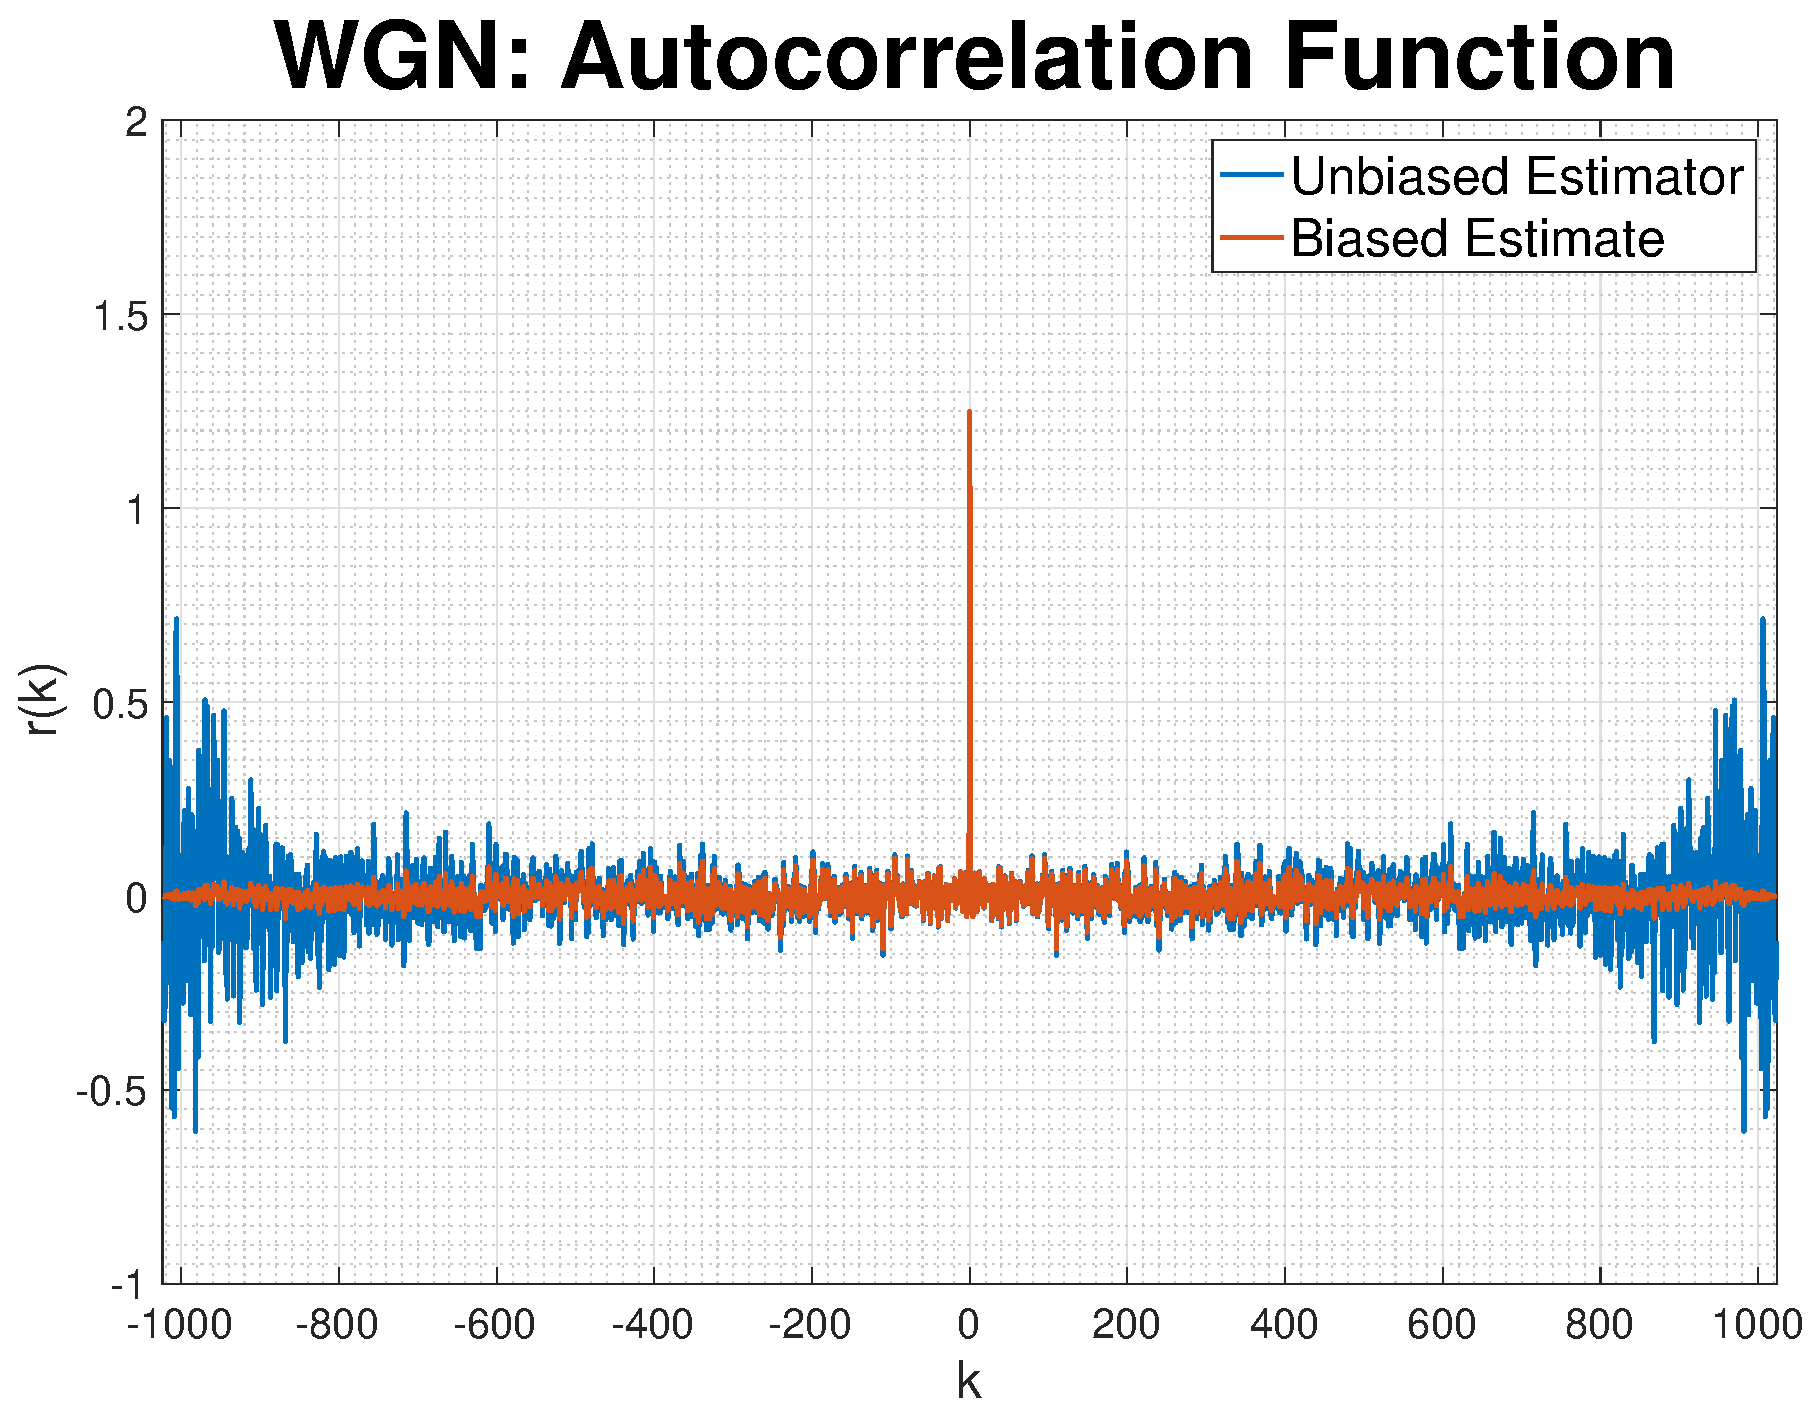
\includegraphics[width=0.32\textwidth]{part2/wgn_biased_and_unbiased_estimates}
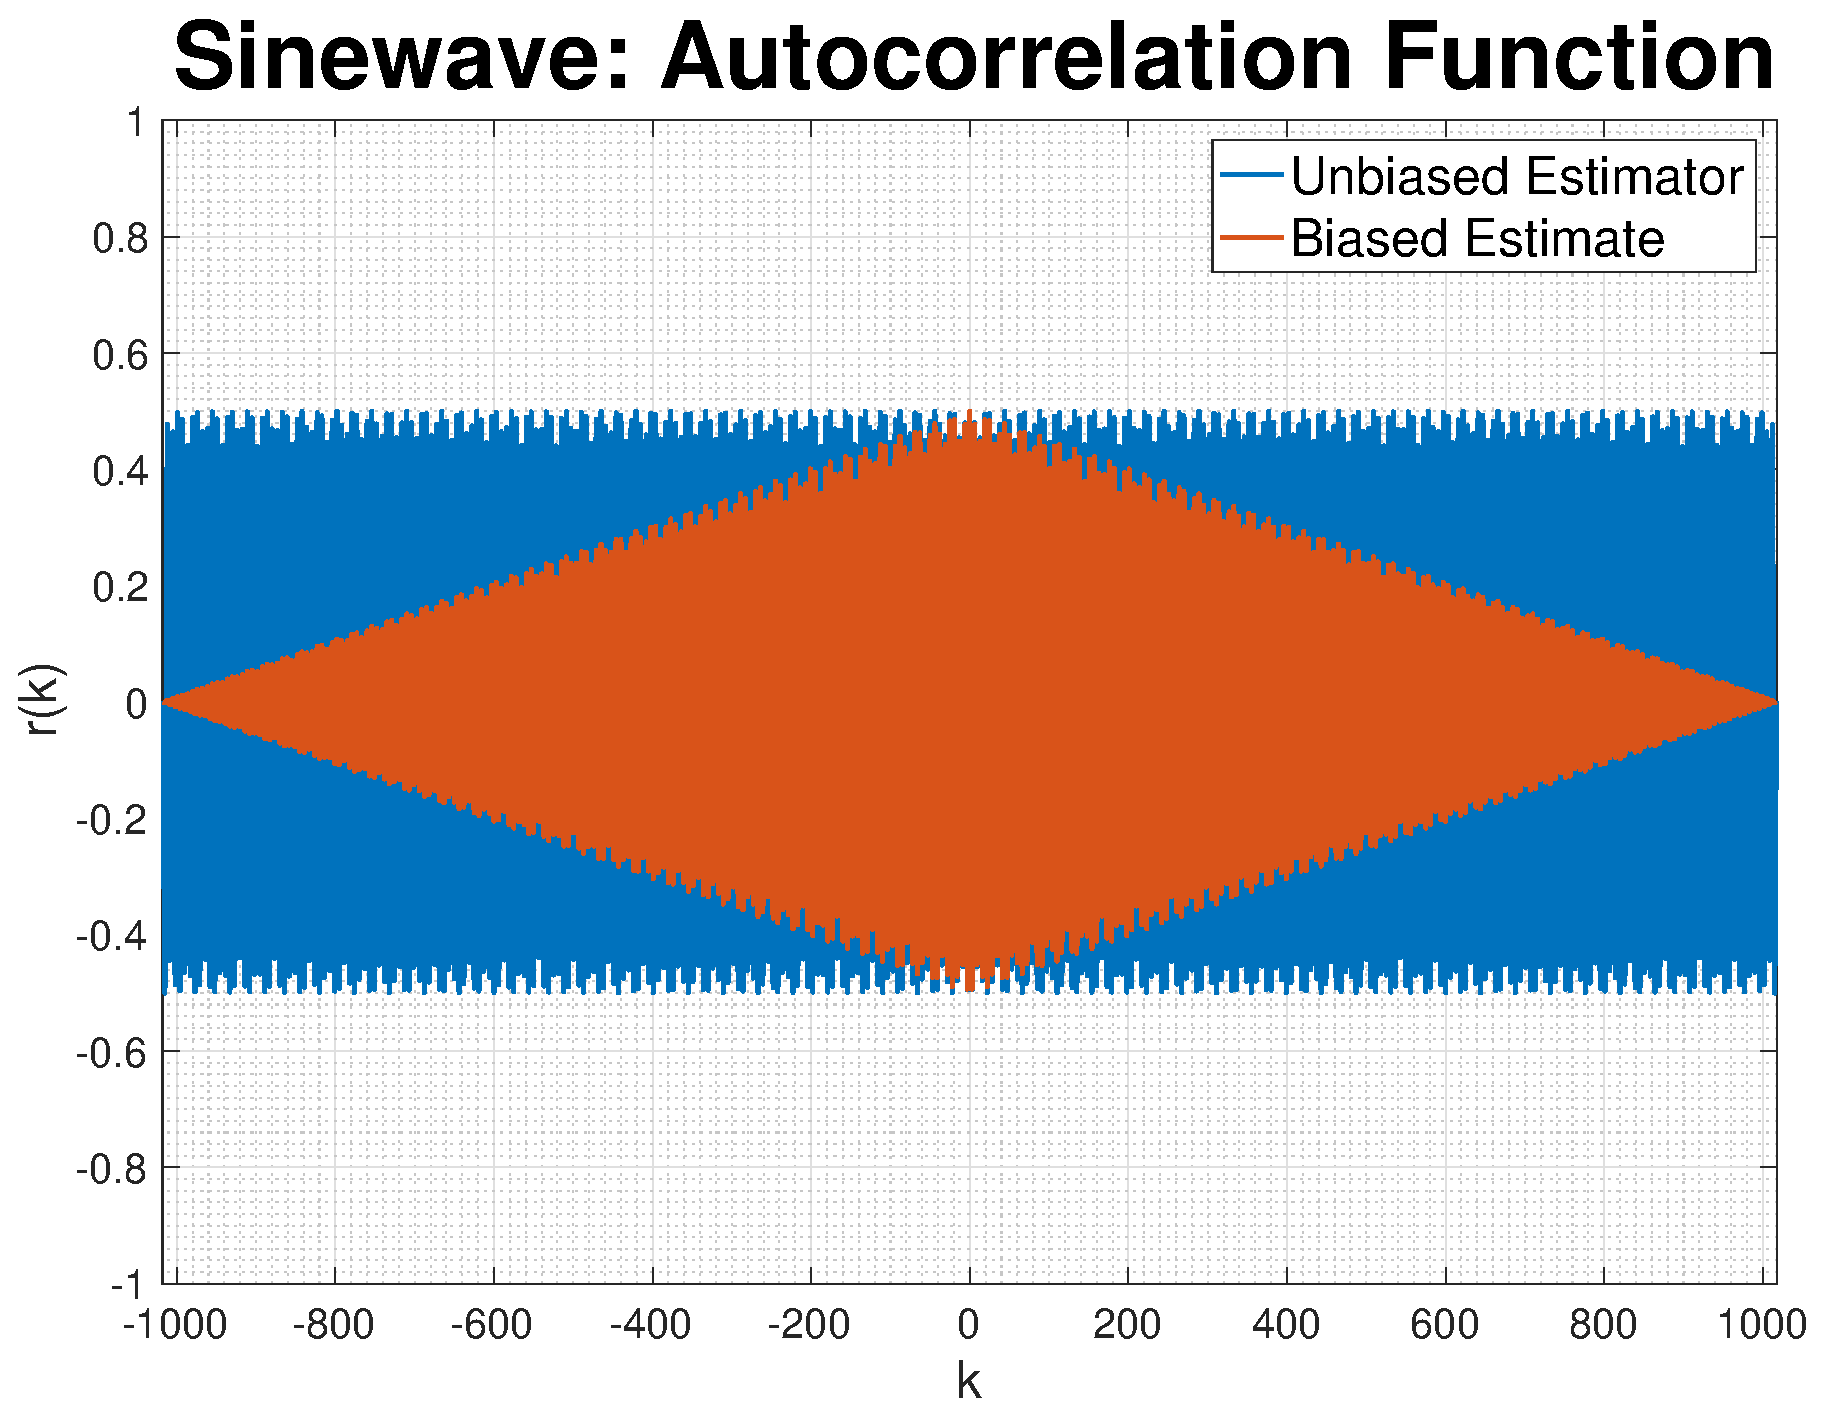
\includegraphics[width=0.32\textwidth]{part2/sinewave_biased_and_unbiased_estimates}
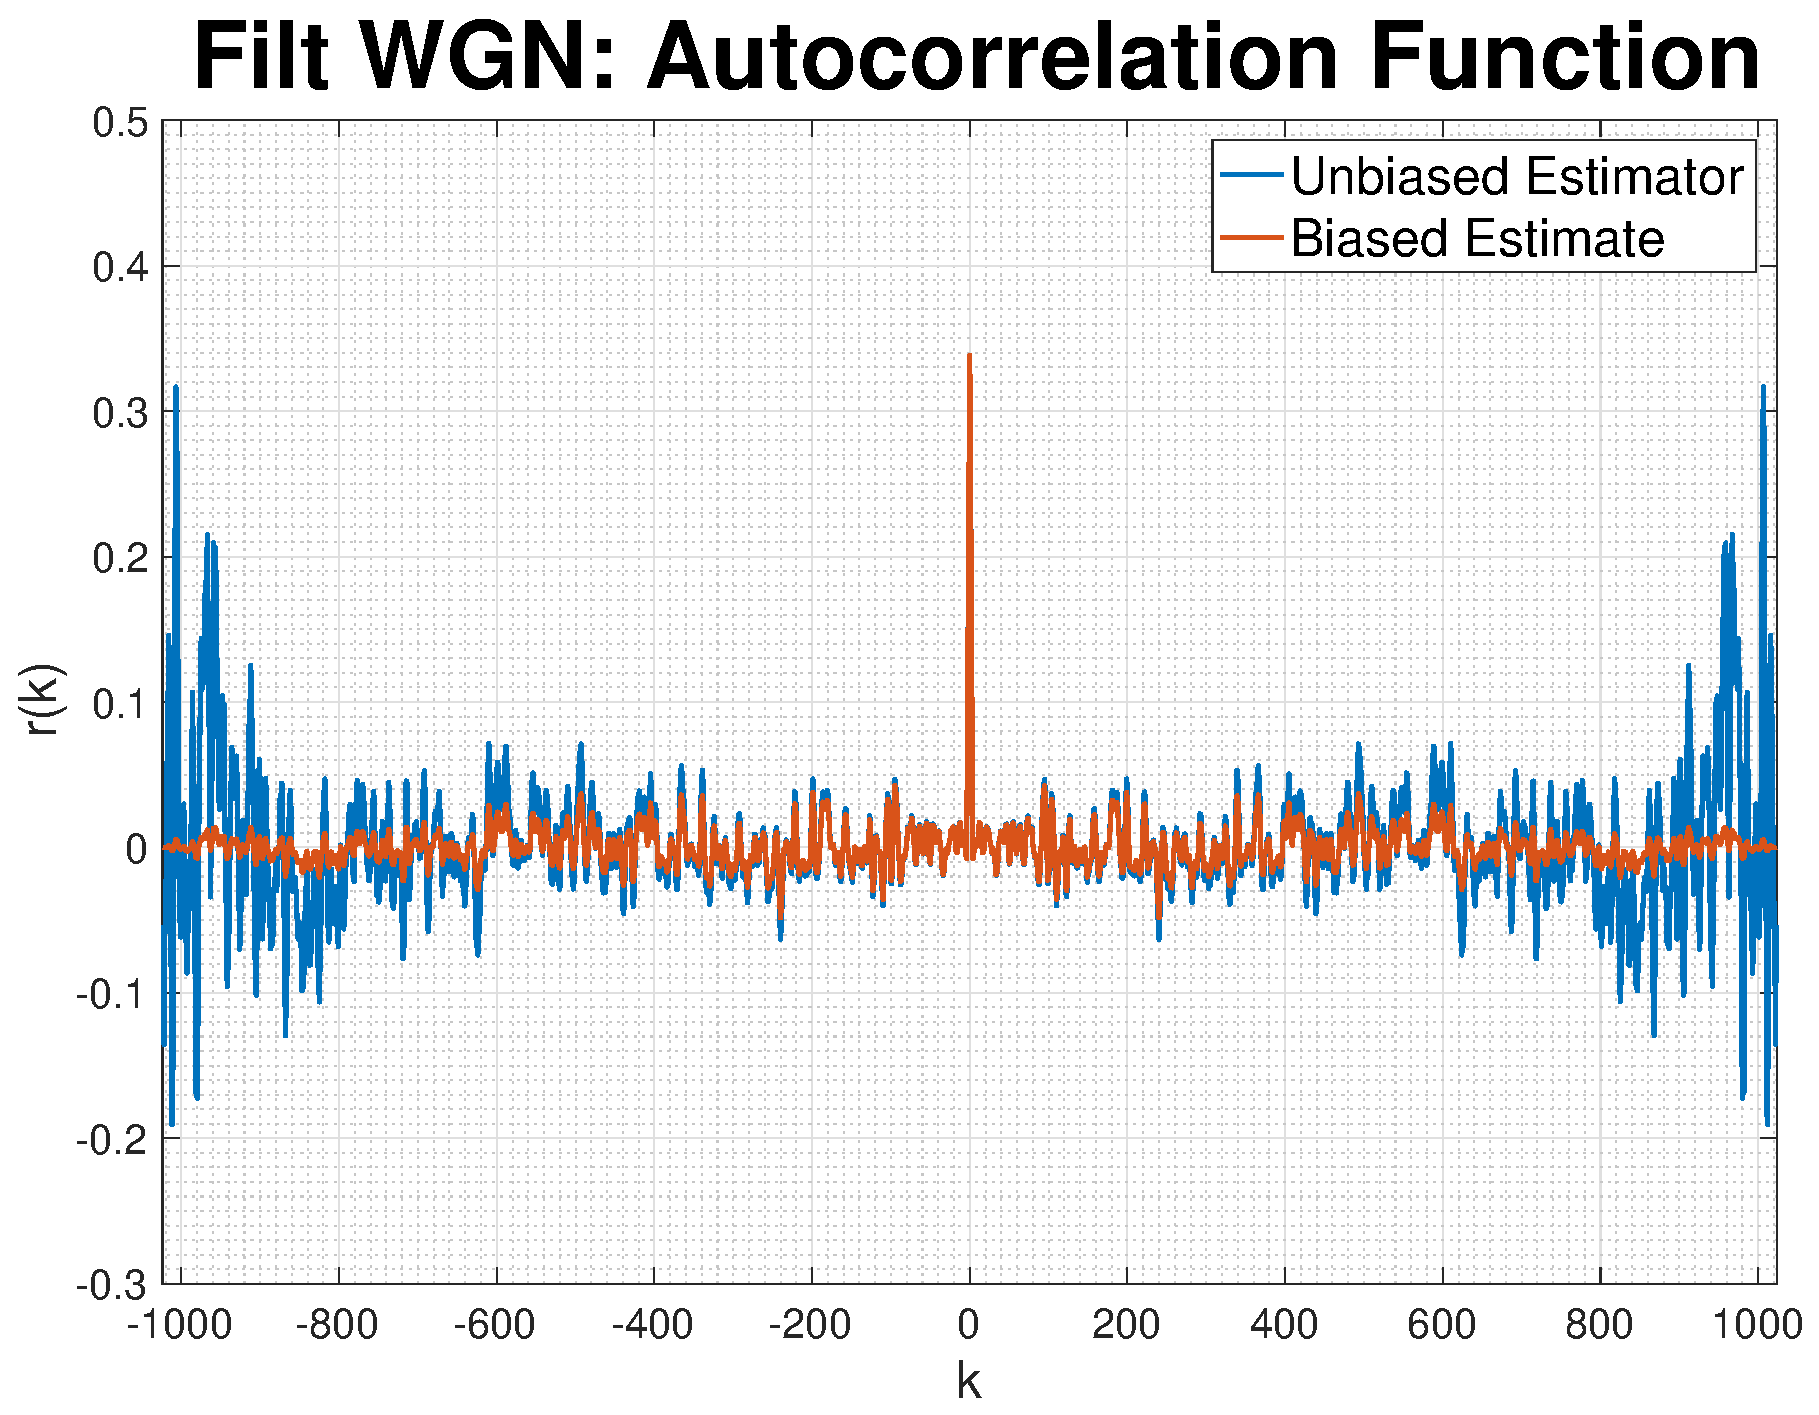
\includegraphics[width=0.32\textwidth]{part2/filt_wgn_biased_and_unbiased_estimates}
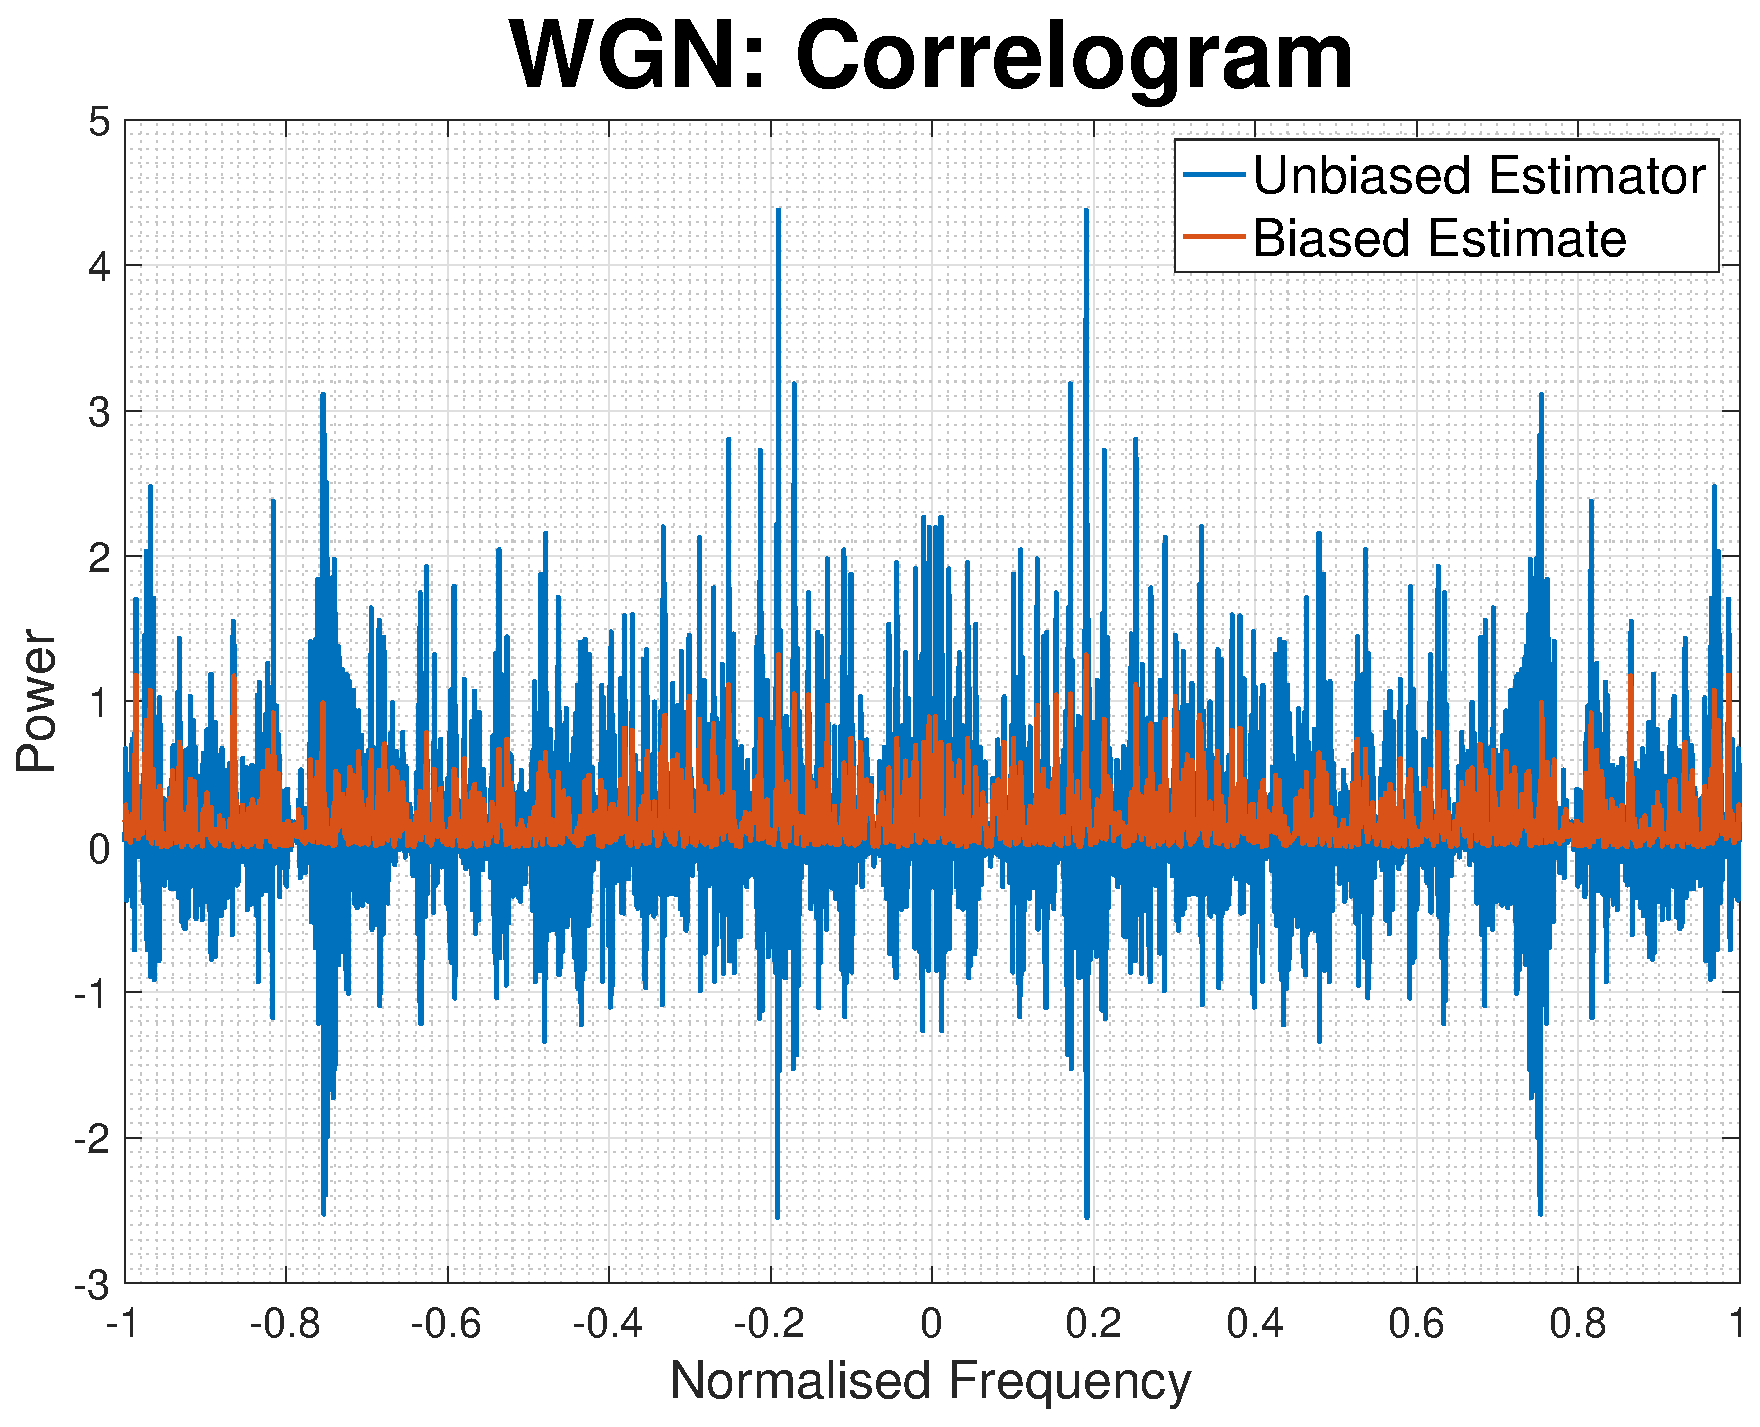
\includegraphics[width=0.32\textwidth]{part2/wgn_correlogram}
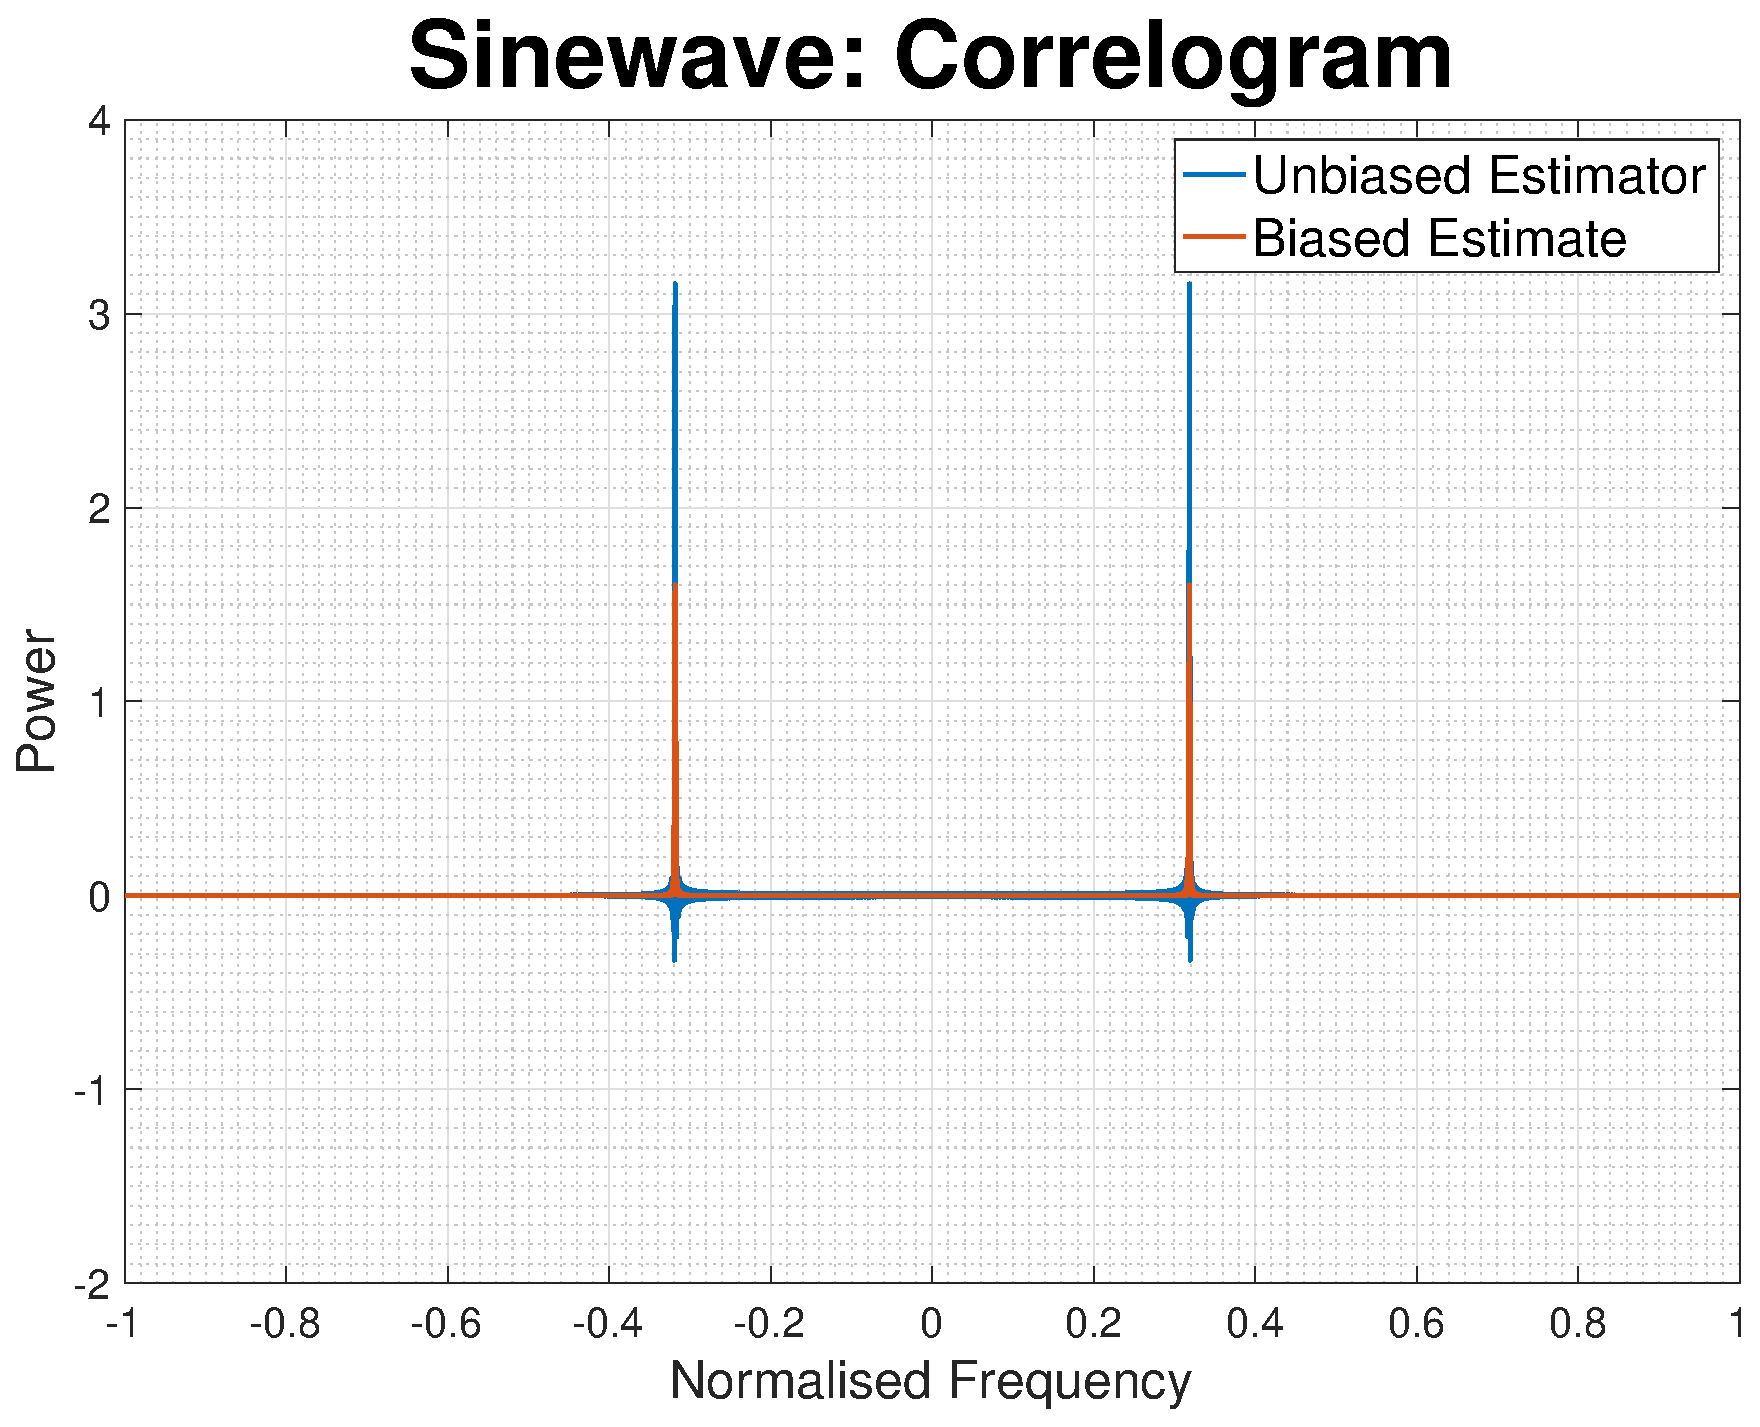
\includegraphics[width=0.32\textwidth]{part2/sinewave_correlogram}
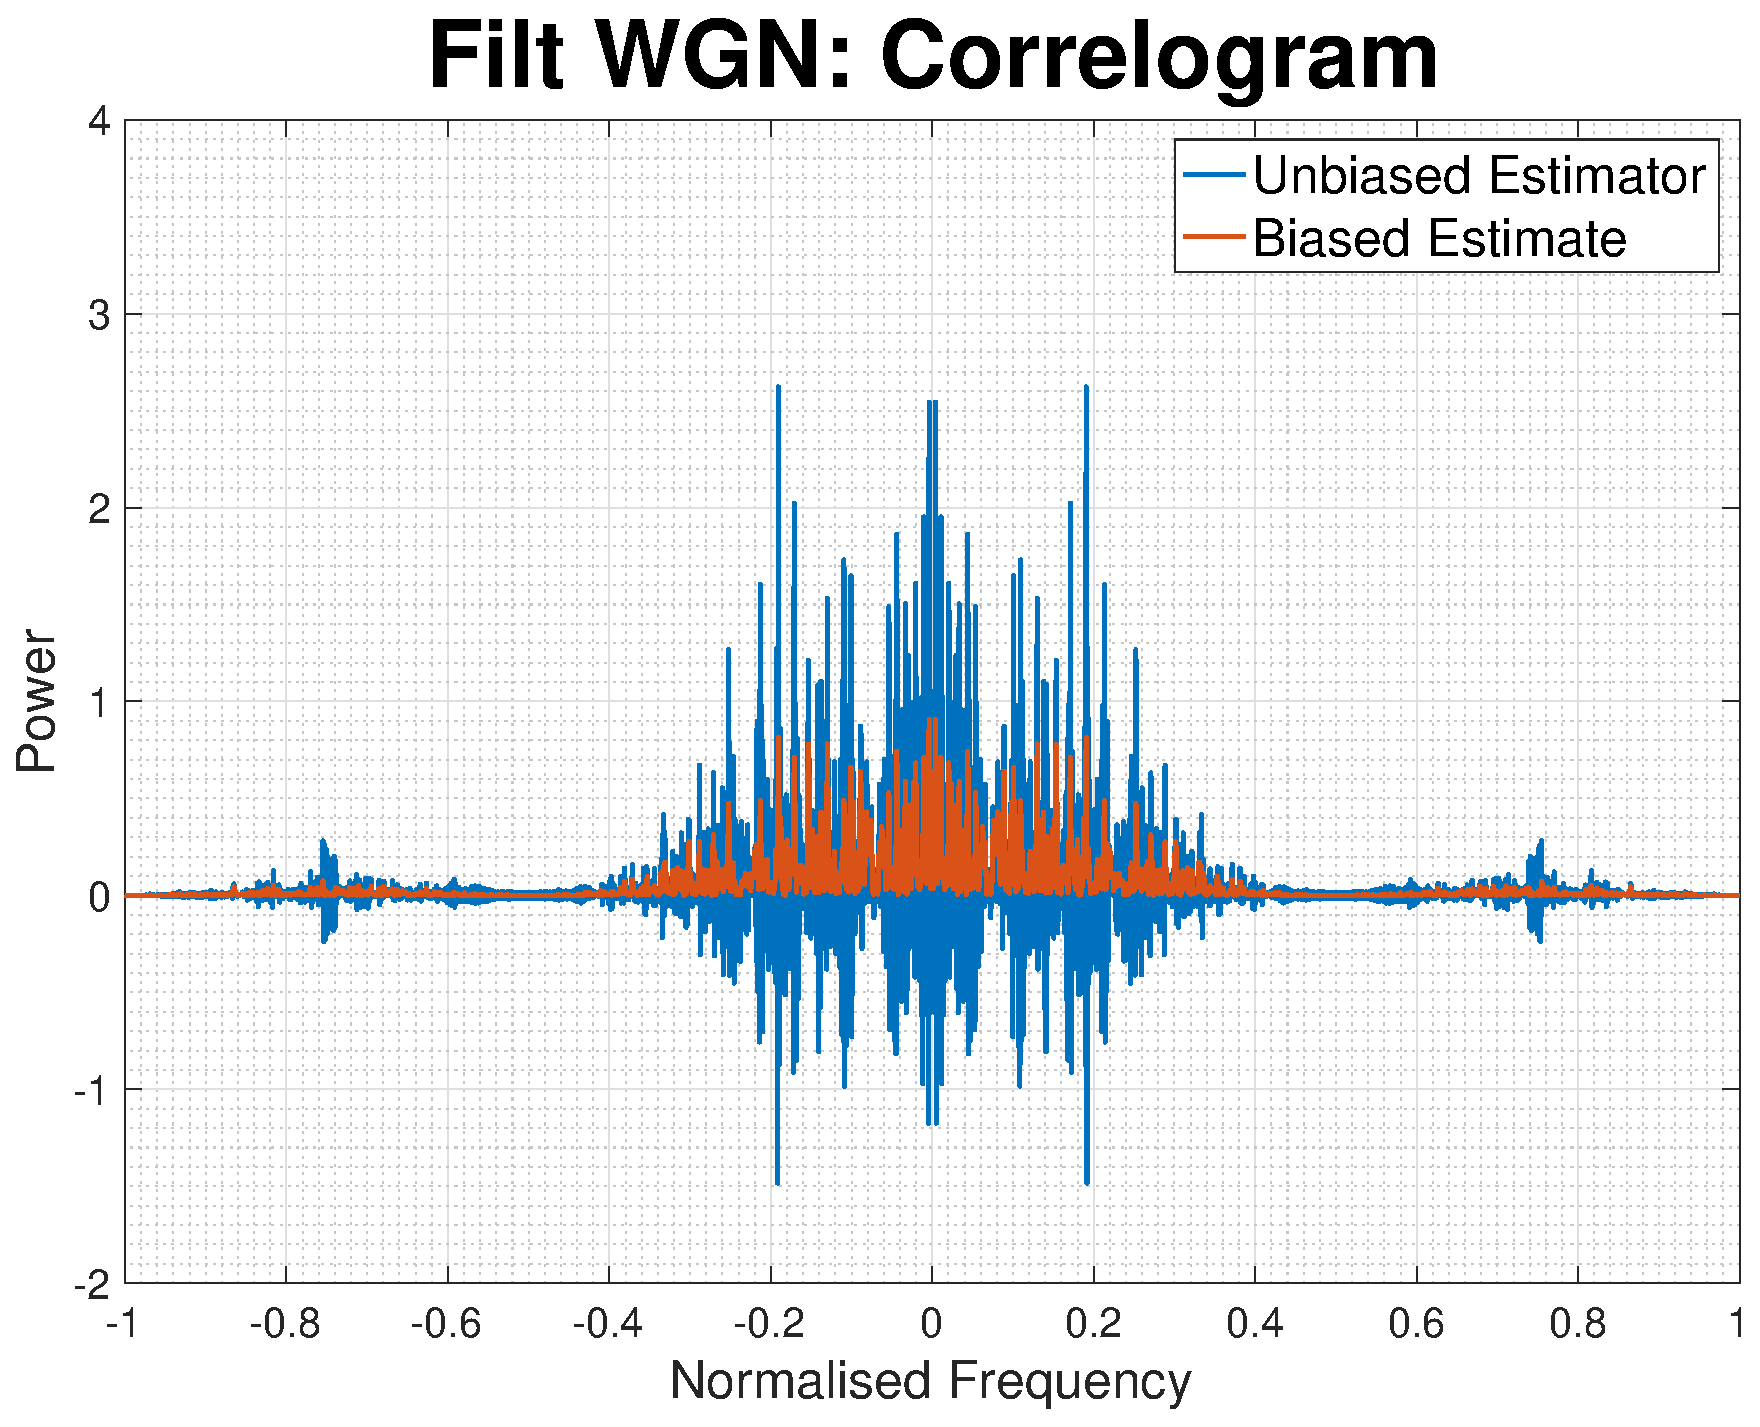
\includegraphics[width=0.32\textwidth]{part2/filt_wgn_correlogram}
\caption{Biased and Unbiased Estimates of ACF and their Effect on the Correlogram}
\label{fig:correlogram}
\end{figure}

\noindent{}b. The figures below show 100 realisations of 2 unique random processes. The mean of the 100 realisations has been graphed in red. It is clear from observing the plots that the random process consist of 2 sine waves each.

\begin{figure}[H]
\centering{}
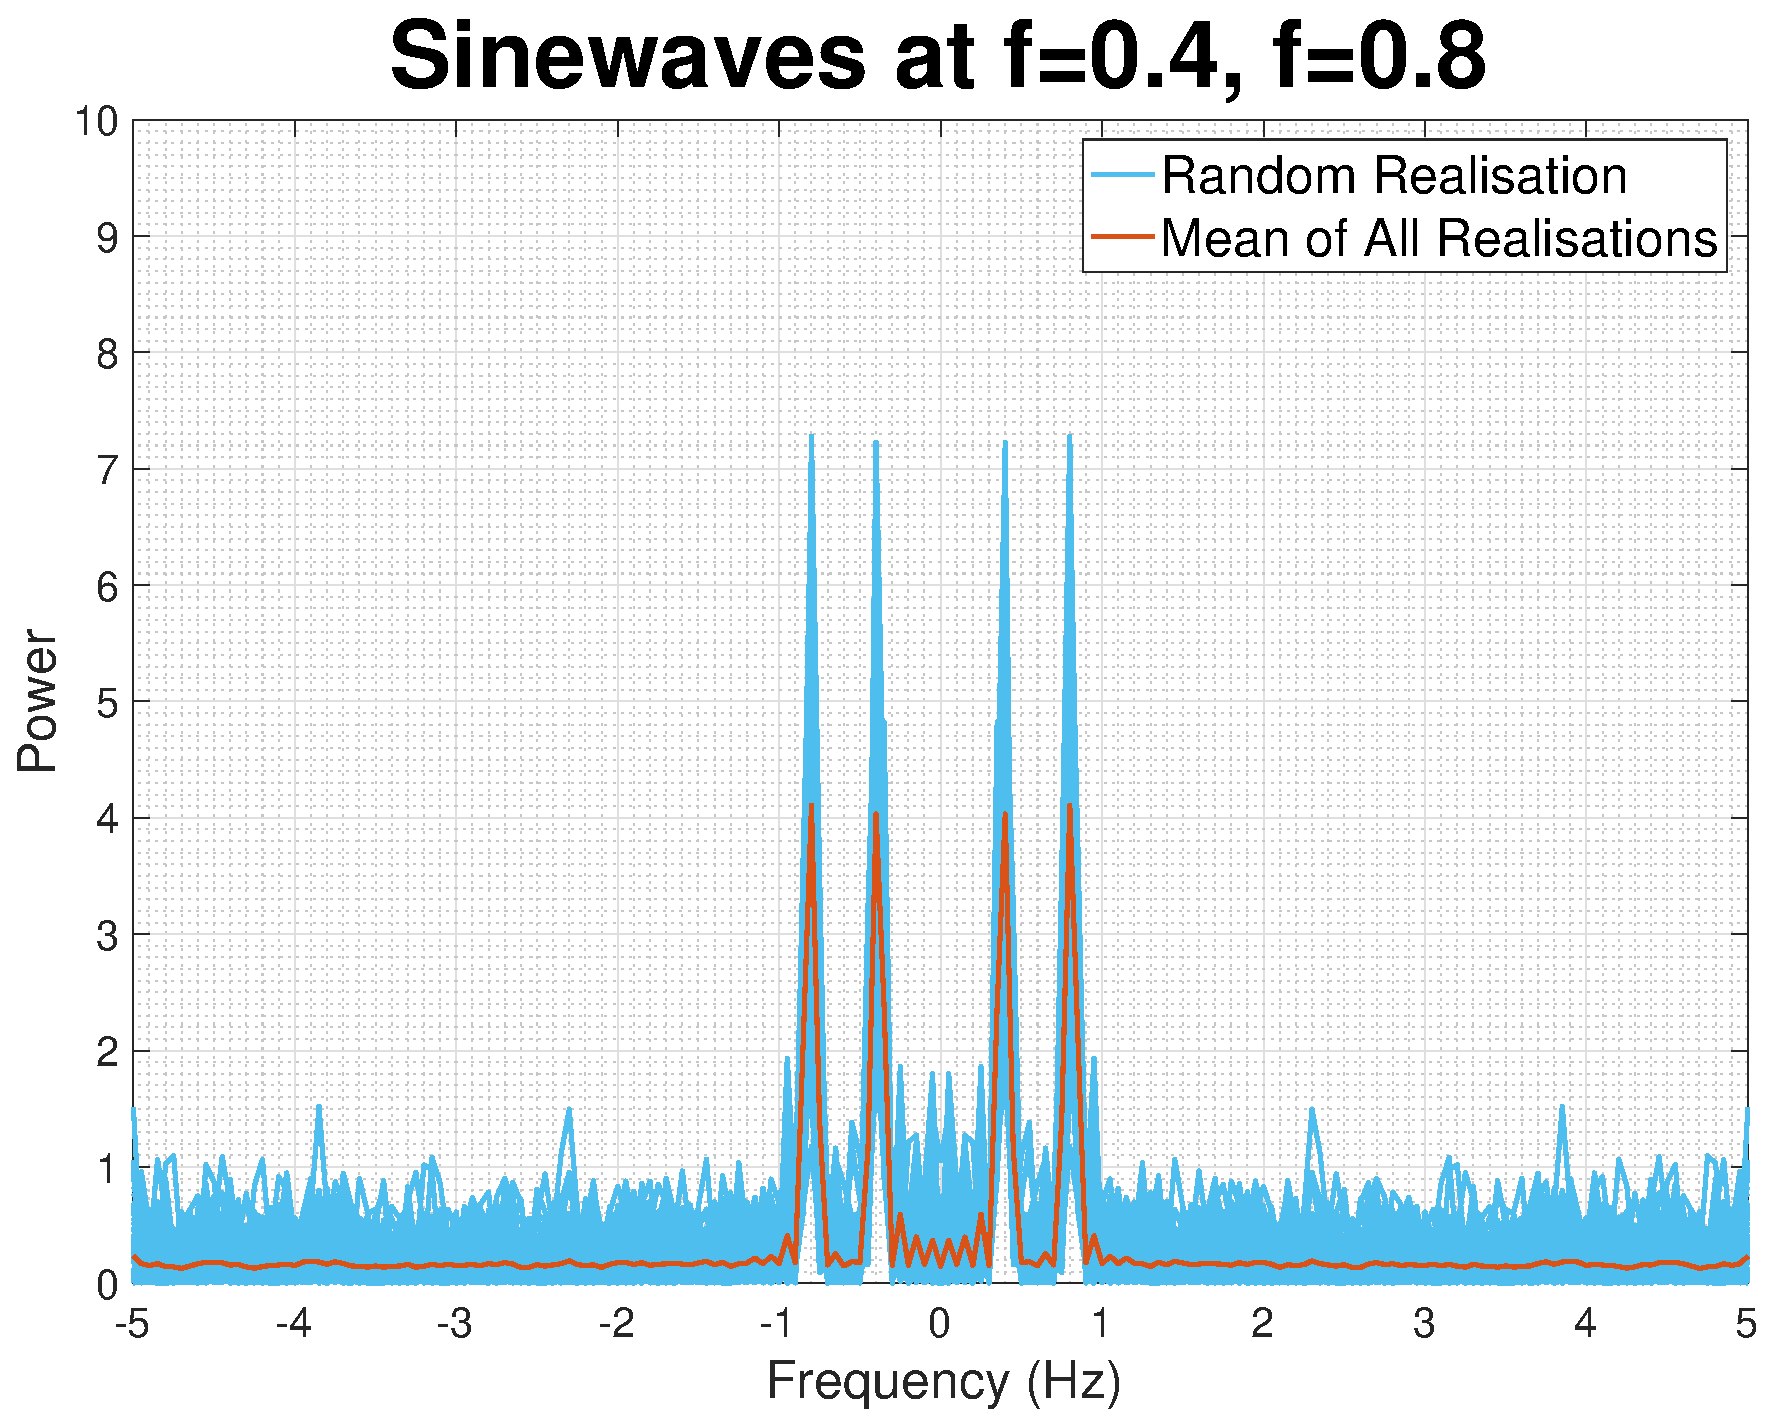
\includegraphics[width=0.32\textwidth]{part2/variance_correlogram_sine_waves_4_8}
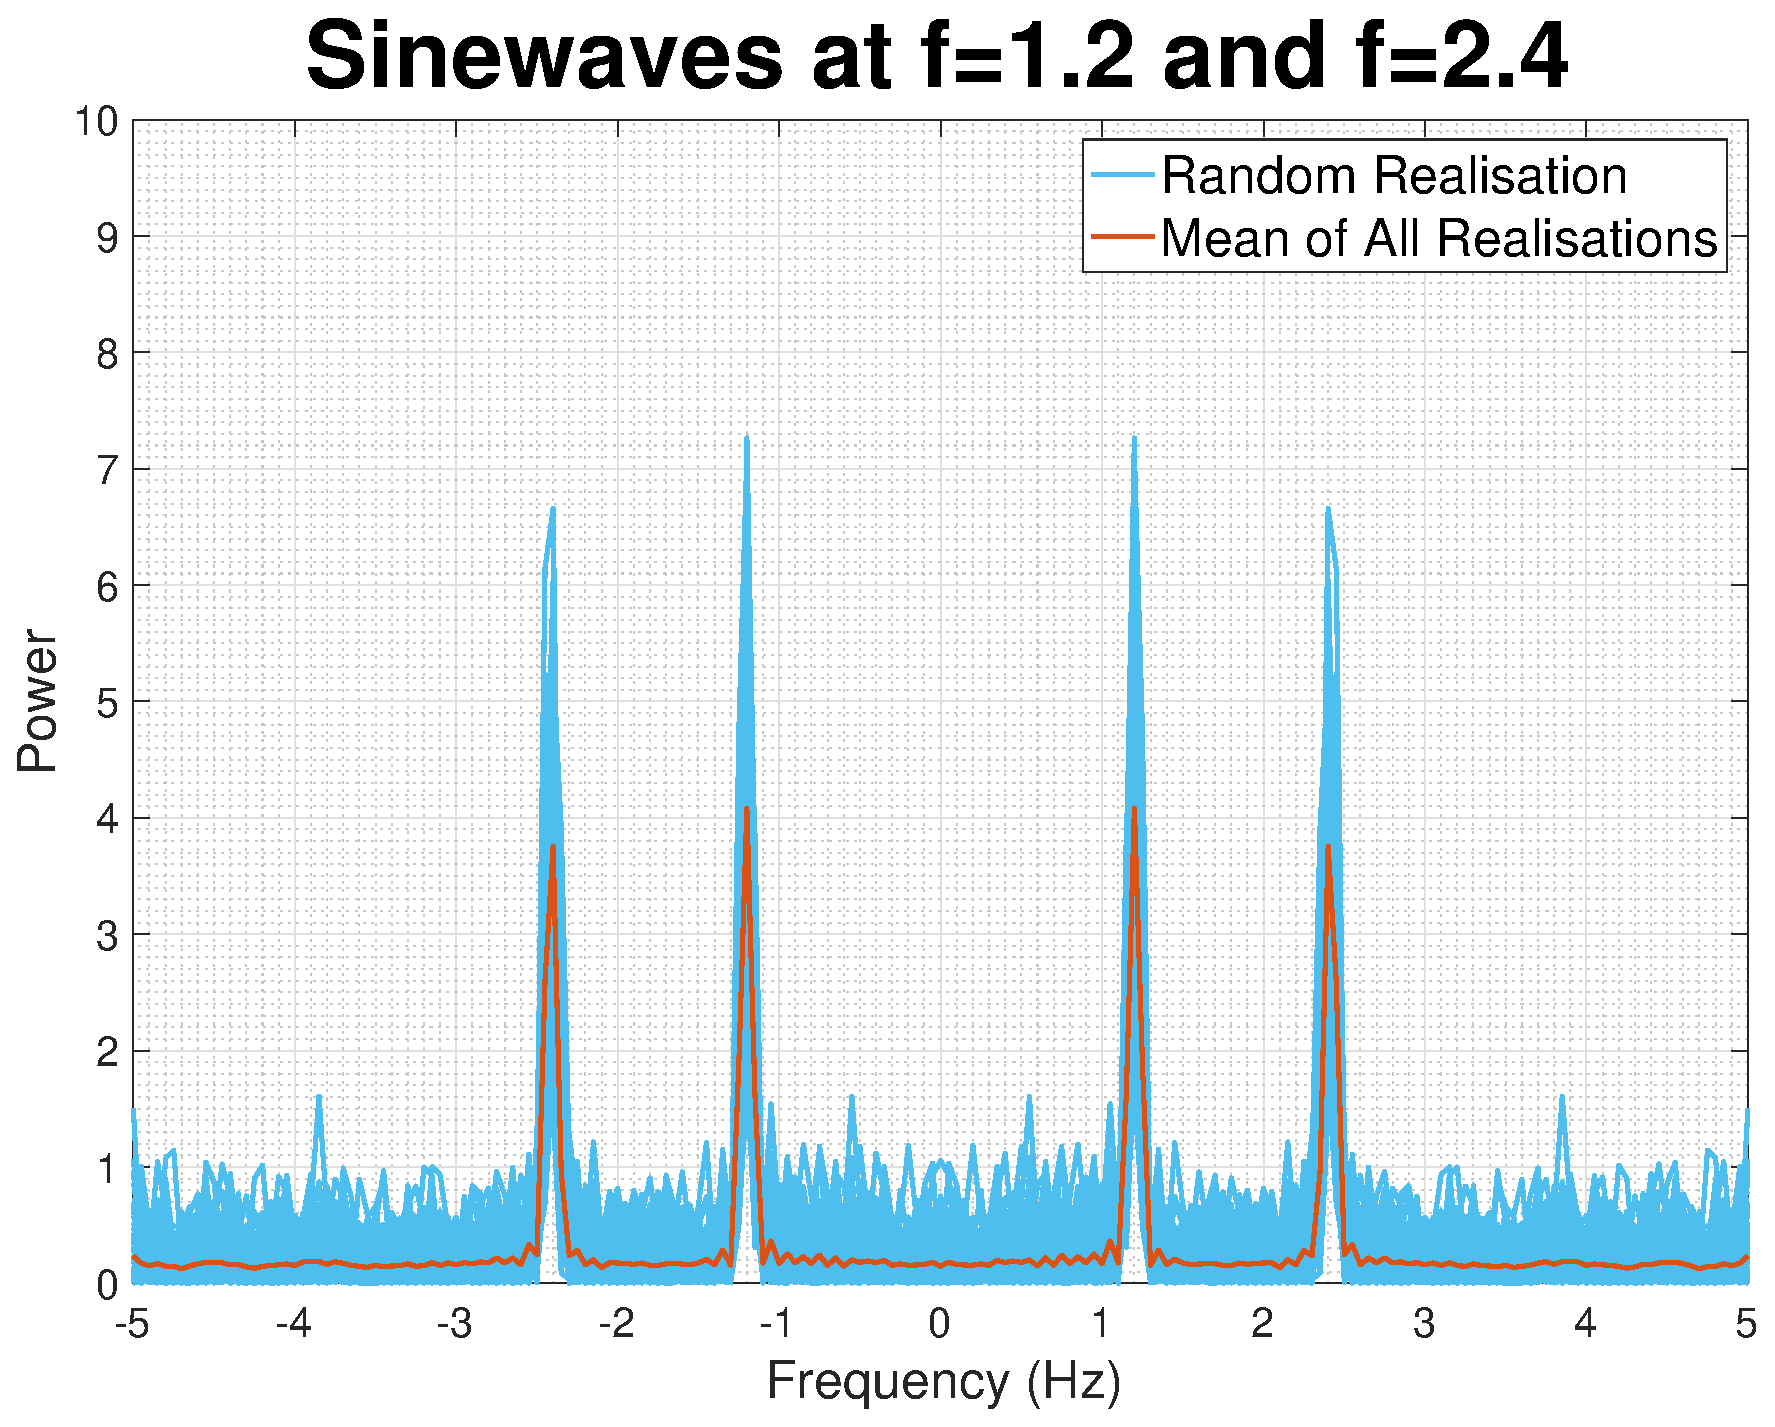
\includegraphics[width=0.32\textwidth]{part2/variance_correlogram_sine_waves_1_2}
\end{figure}

\begin{figure}[H]
\centering{}
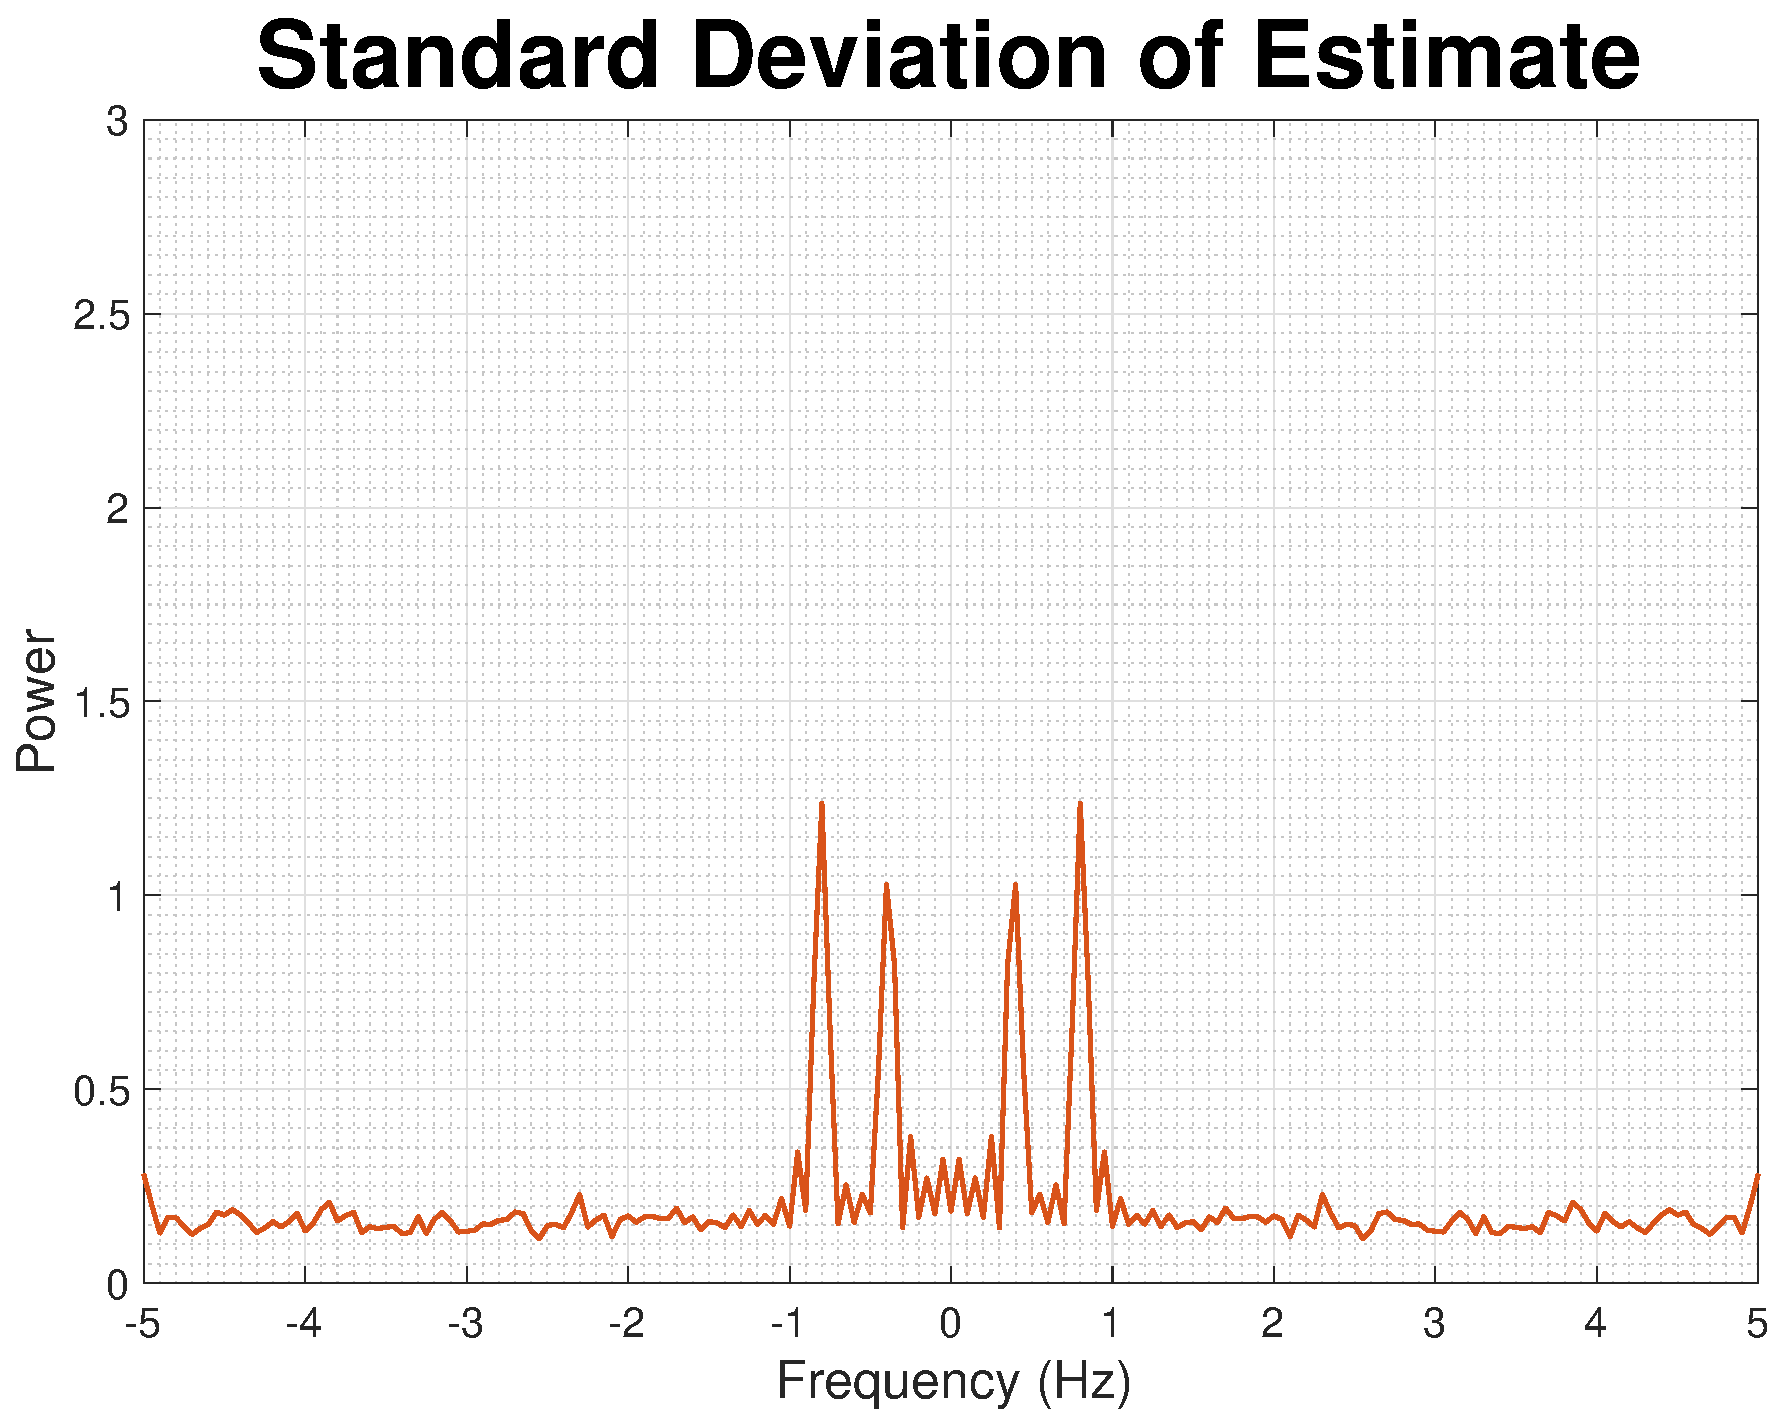
\includegraphics[width=0.32\textwidth]{part2/std_dev_correlogram_sine_waves_4_8}
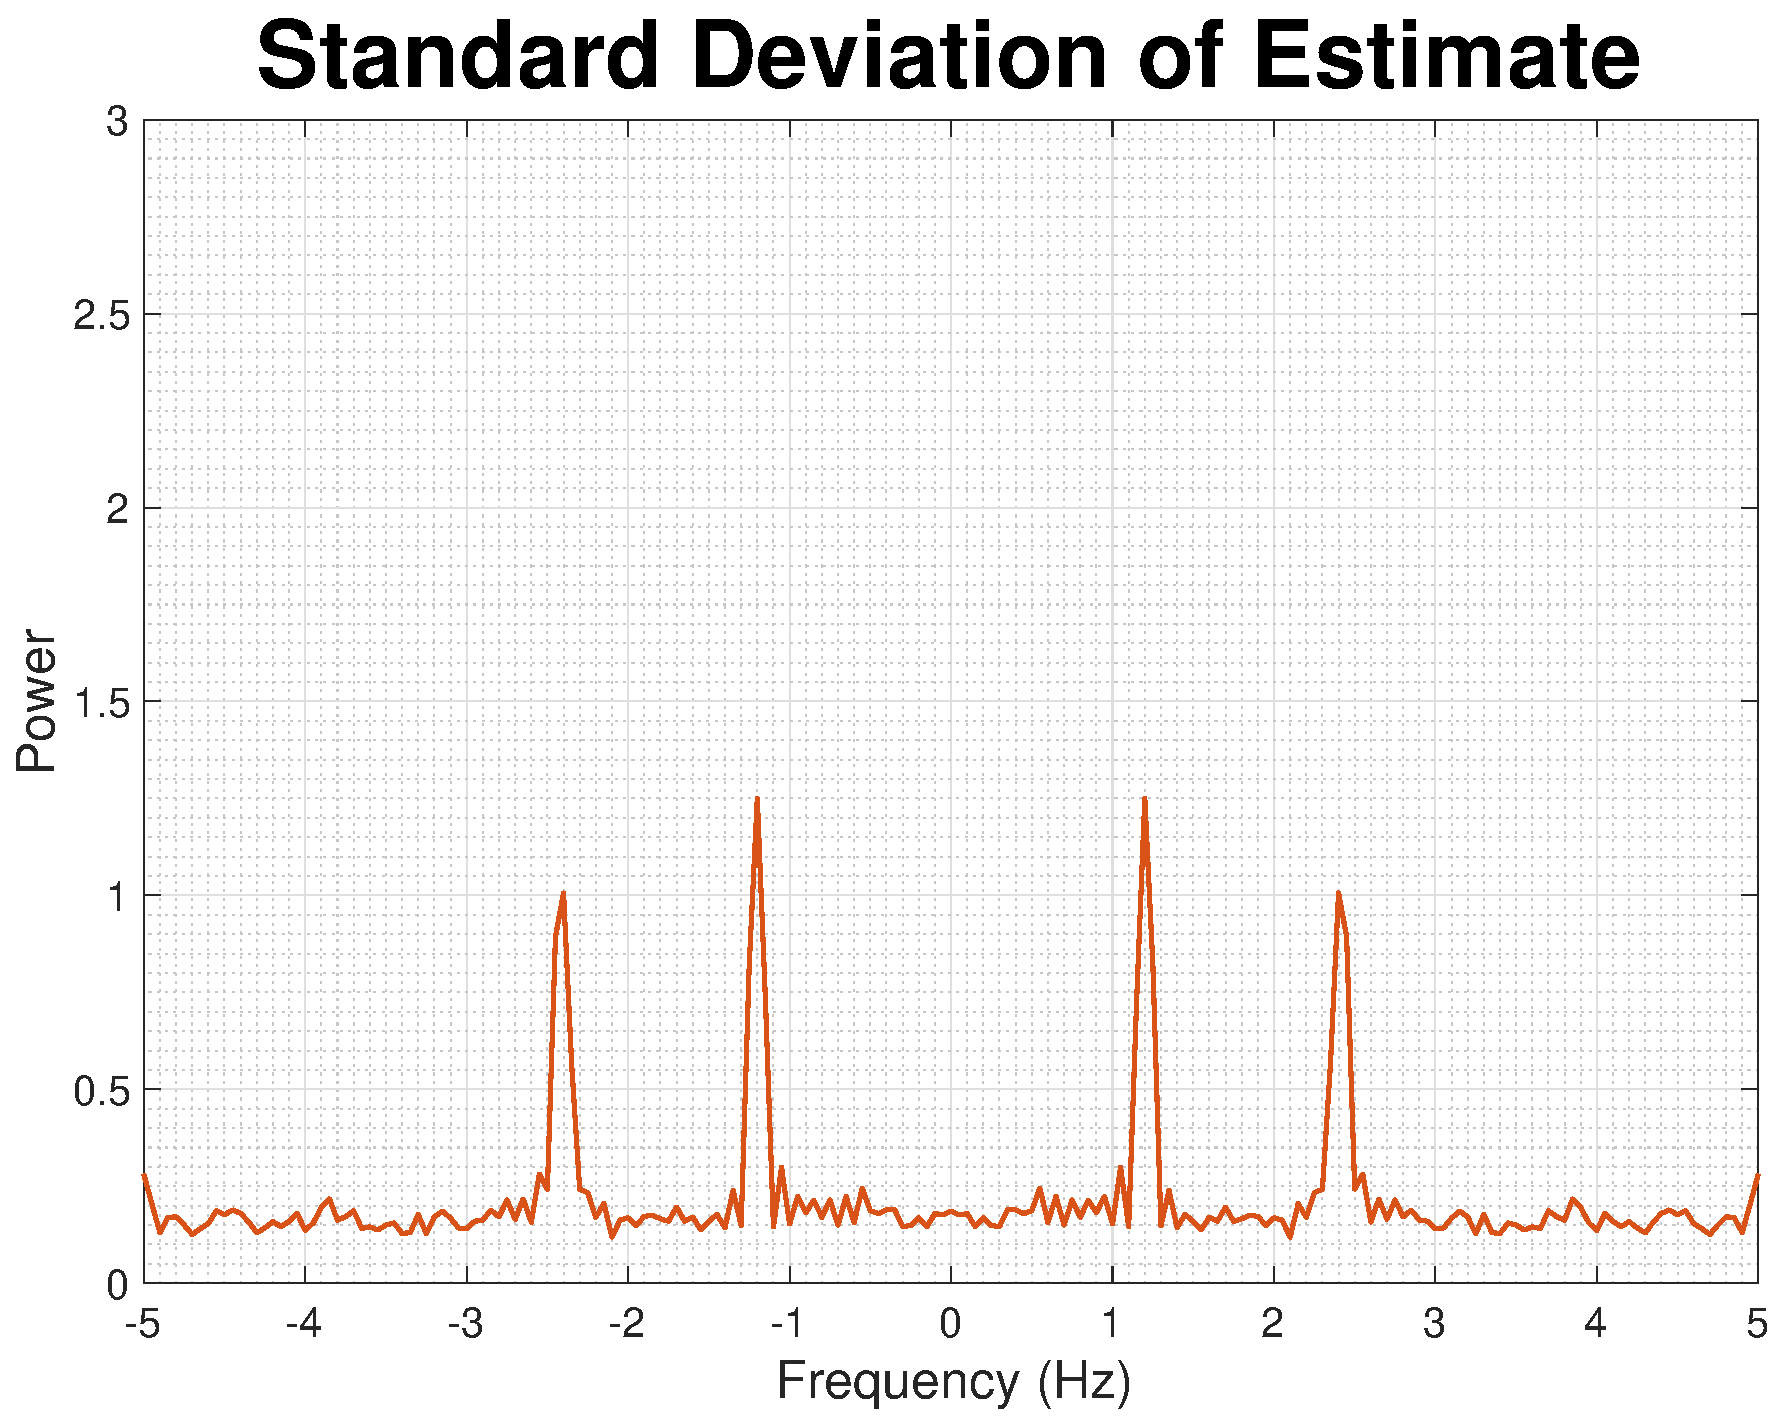
\includegraphics[width=0.32\textwidth]{part2/std_dev_correlogram_sine_waves_1_2}
\caption{Variance and Standard Deviation of Correlogram Spectral Estimates}
\end{figure}

\noindent{}The figure above also includes the standard deviate of the 100 spectral estimates. Notice that there are peaks in the standard deviate at exactly the same frequencies as the peaks in the periodogram estimates. This is indicative of one of the short-comings on the periodogram spectral estimator. \textbf{The periodogram is not a consistent estimator.} For it to be consistent, $\text{var}(P_{per}) \rightarrow 0  \ \text{as} \ N \rightarrow \infty$. The peridogoram does not statisfy that condition but instead,  $\text{var}(P_{per}) \rightarrow P_{x}^{2}(f) \ \text{as} \ N \rightarrow \infty$. This is clearly depecited in the plots of standard deviation below; it spikes at $f=0.4, 0.8$ Hz and $f=1.2, 2.4$ Hz. Thus, simply collecting more samples and then calculating the peirodogram will not reduce variance. Other methods such as the Blackman-Tukey must be considered if variance is to be reduced.\\

\noindent{}c. Notice that when the graphs are plotted in the dB, the effects described above are made even more obvious. It is interesting to note that the effects of windowing the sinewave are now also clear. Notice the $sinc^2$ like shape near the peaks at $f=1.2, 2.4$ Hz.
 
\begin{figure}[H]
\centering{}
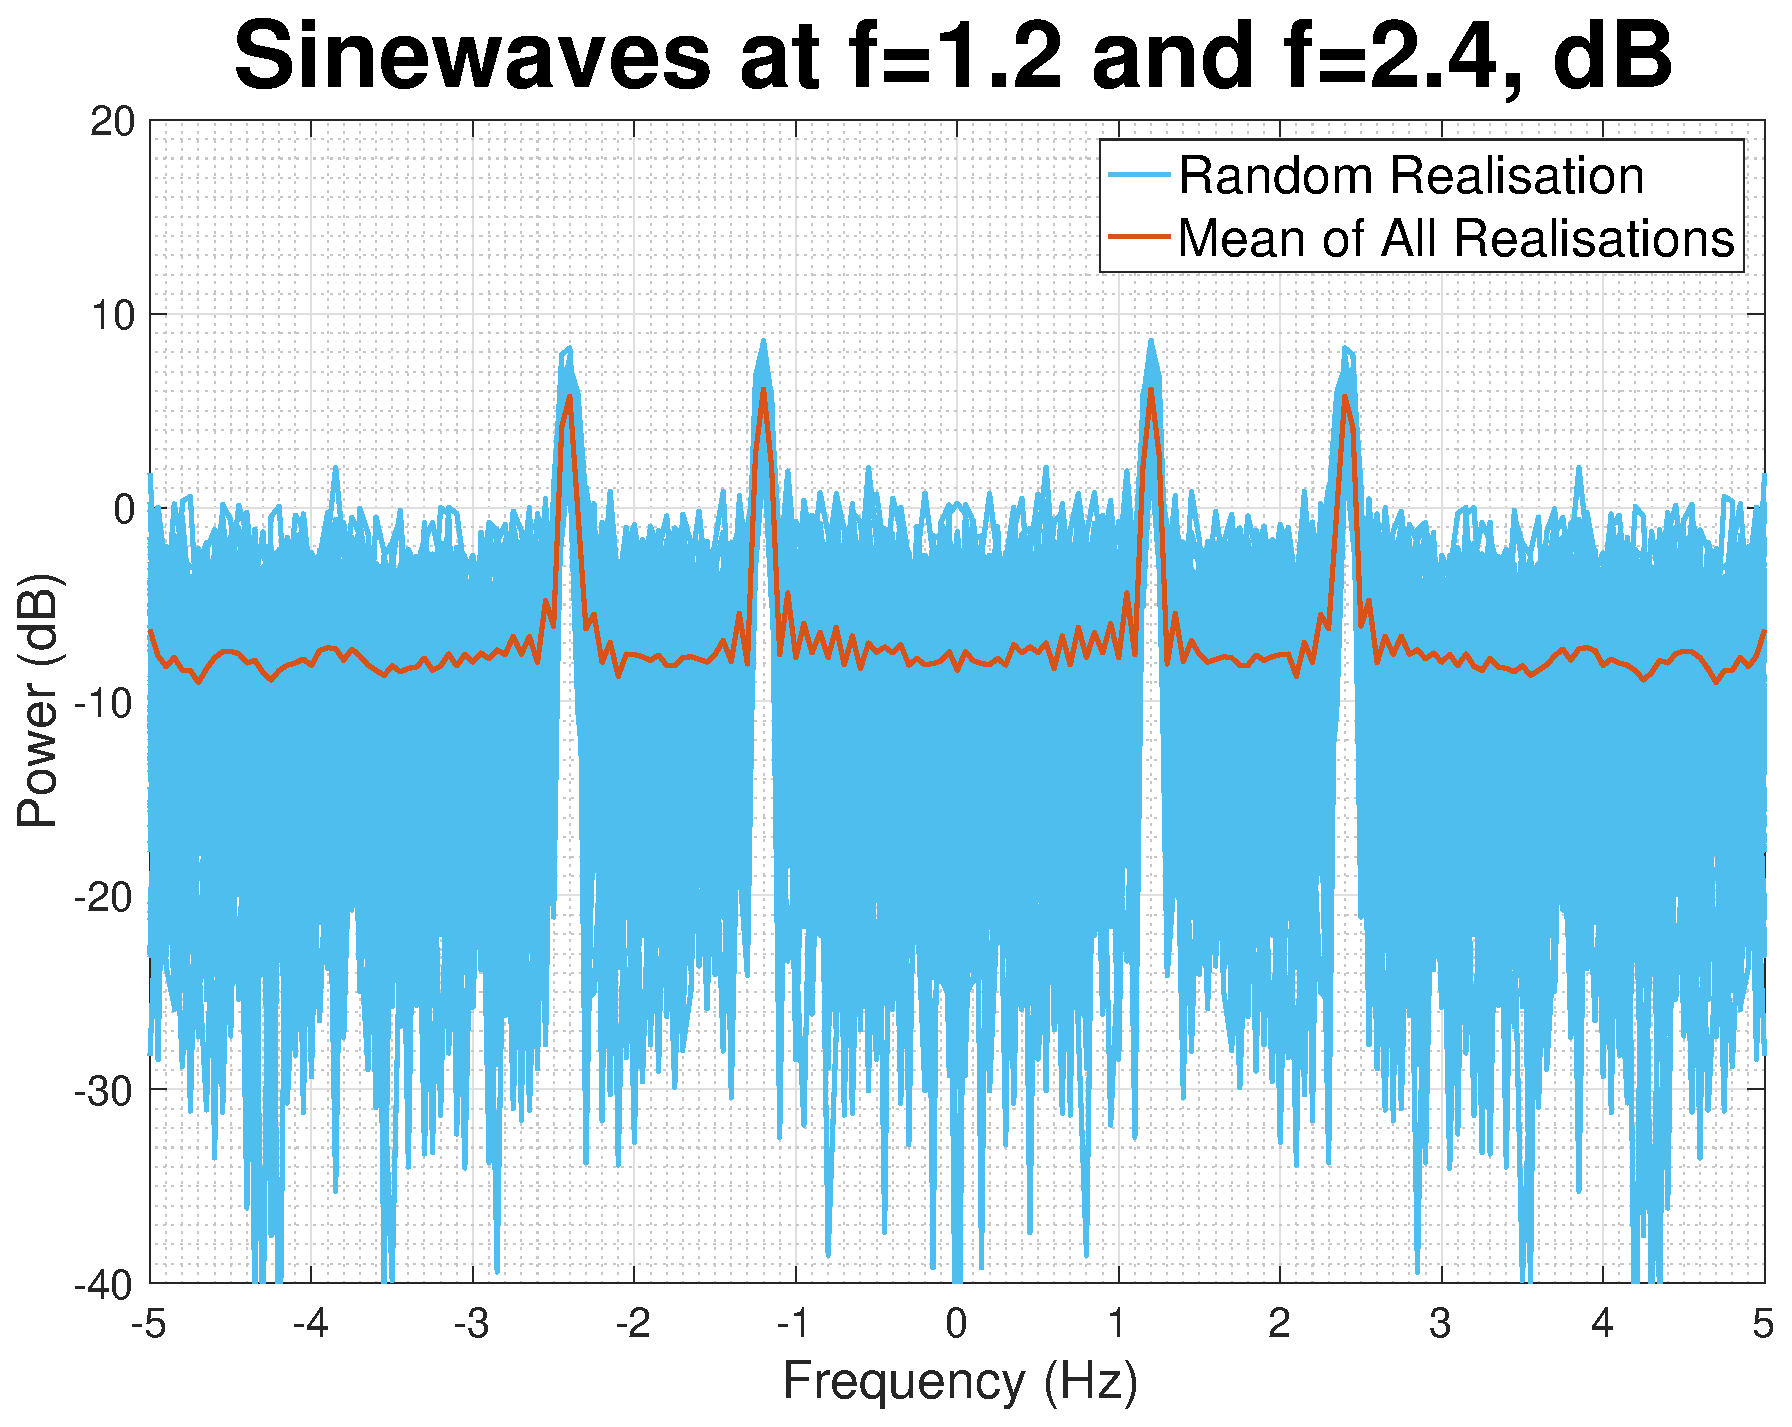
\includegraphics[width=0.32\textwidth]{part2/variance_correlogram_sine_waves_1_2_dB}
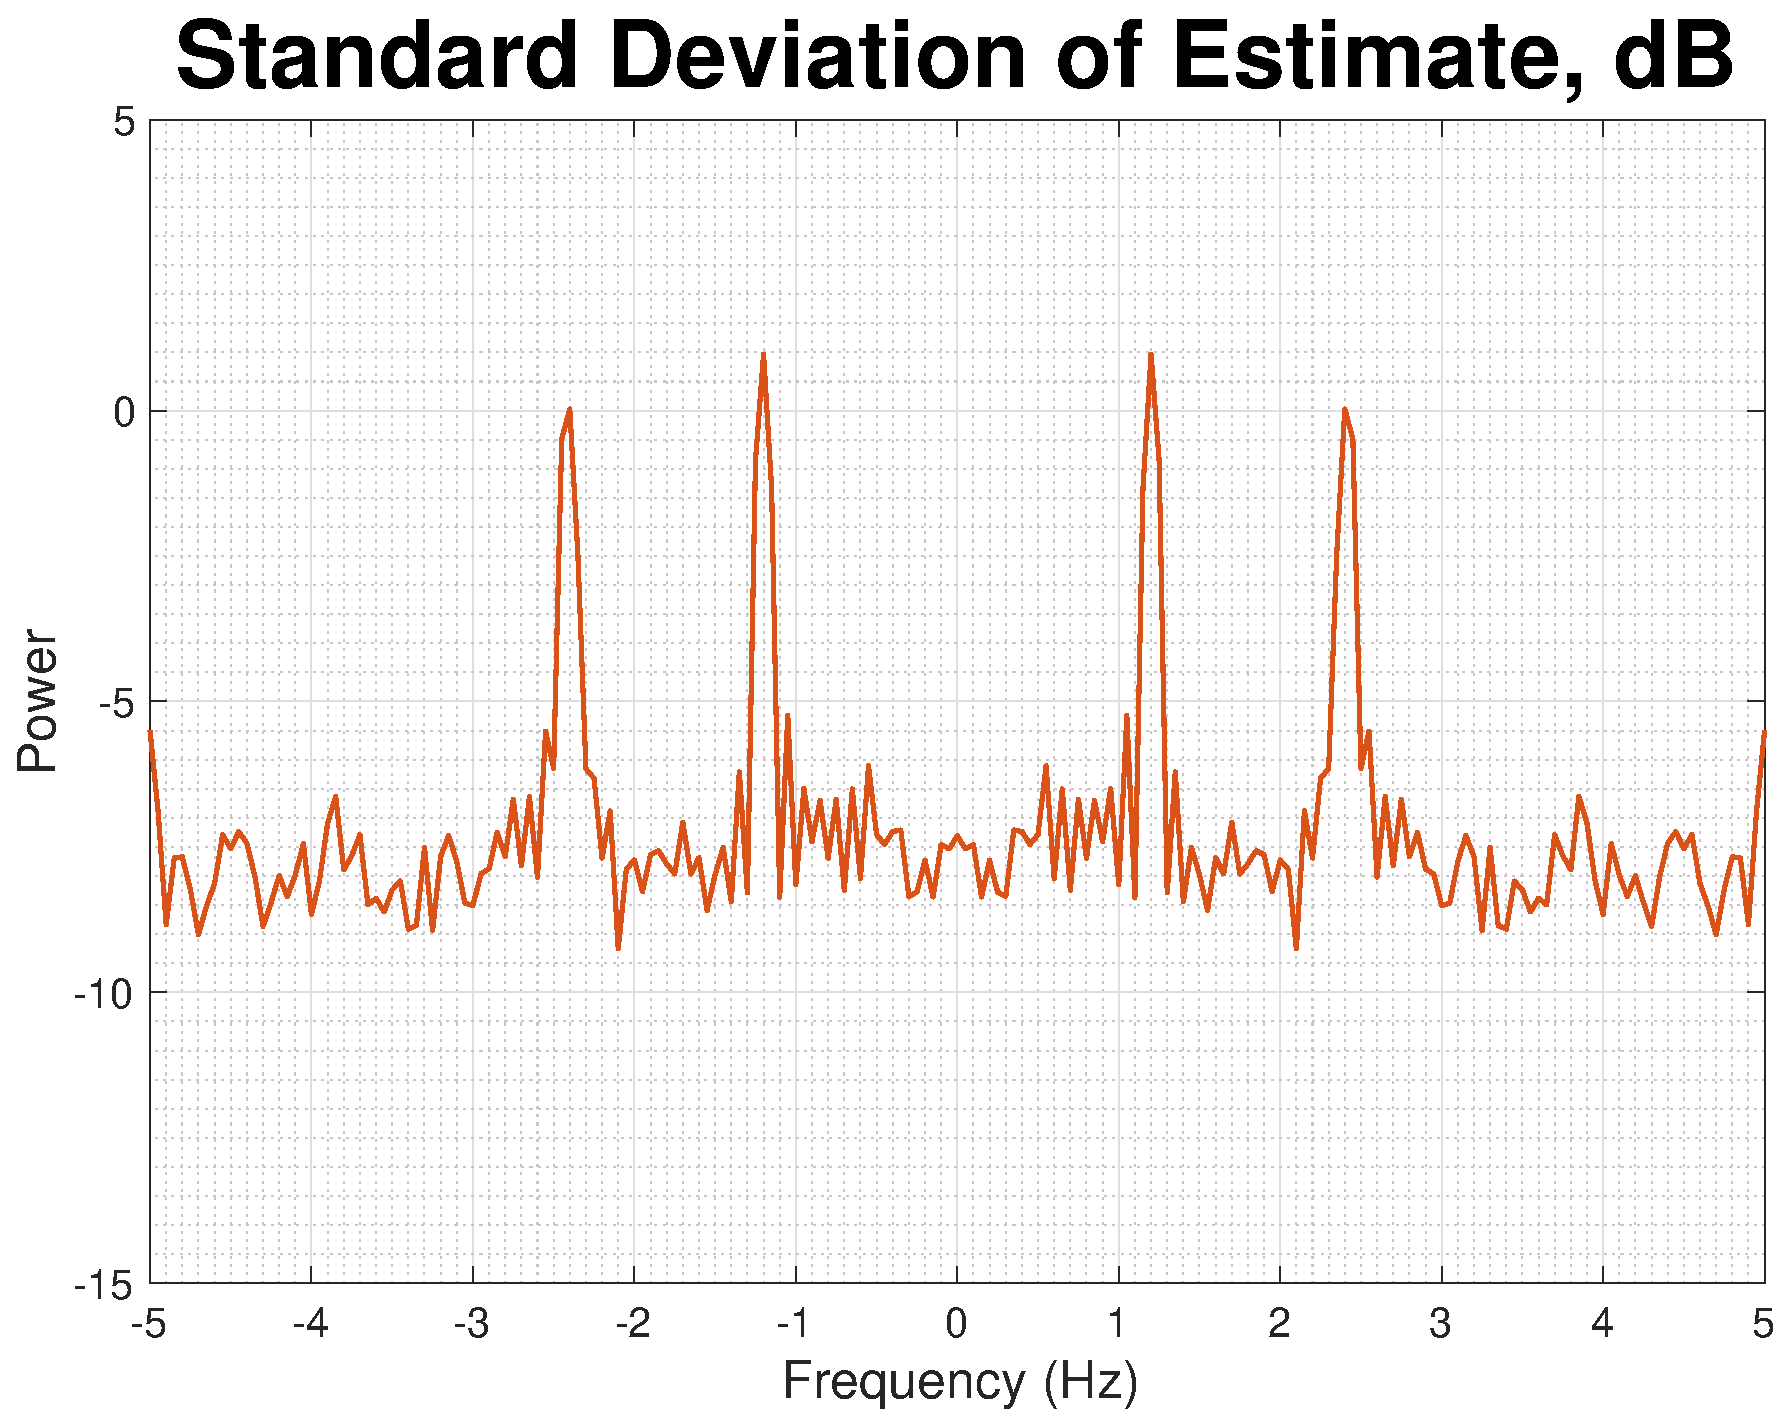
\includegraphics[width=0.32\textwidth]{part2/std_dev_correlogram_sine_waves_1_2_dB}
\caption{Effect of dB Scale on Spread of Variance and Standard Deviation of Correlogram Spectral Estimates}
\end{figure}

\noindent{}d. Since the frequency resolution of the periodogram is proportional to $\frac{1}{N}$, we expect to be able to distinguish 2 complex exponentials with frequencies of $0.3$ Hz and $0.32$ Hz with approximately $50$ samples; with $50$ samples, we will have a resolution of approximately $0.02$ Hz. The figures below confirm this cans show that as the number of samples increases, the ability to distinguish the peaks increases. Note that the periodograms are no longer only symmetric, since the functions are complex, and thus the one-sided periodogram is plotted up to $f_s$ instead of $\frac{f_s}{2}$.

\begin{figure}[H]
\centering{}
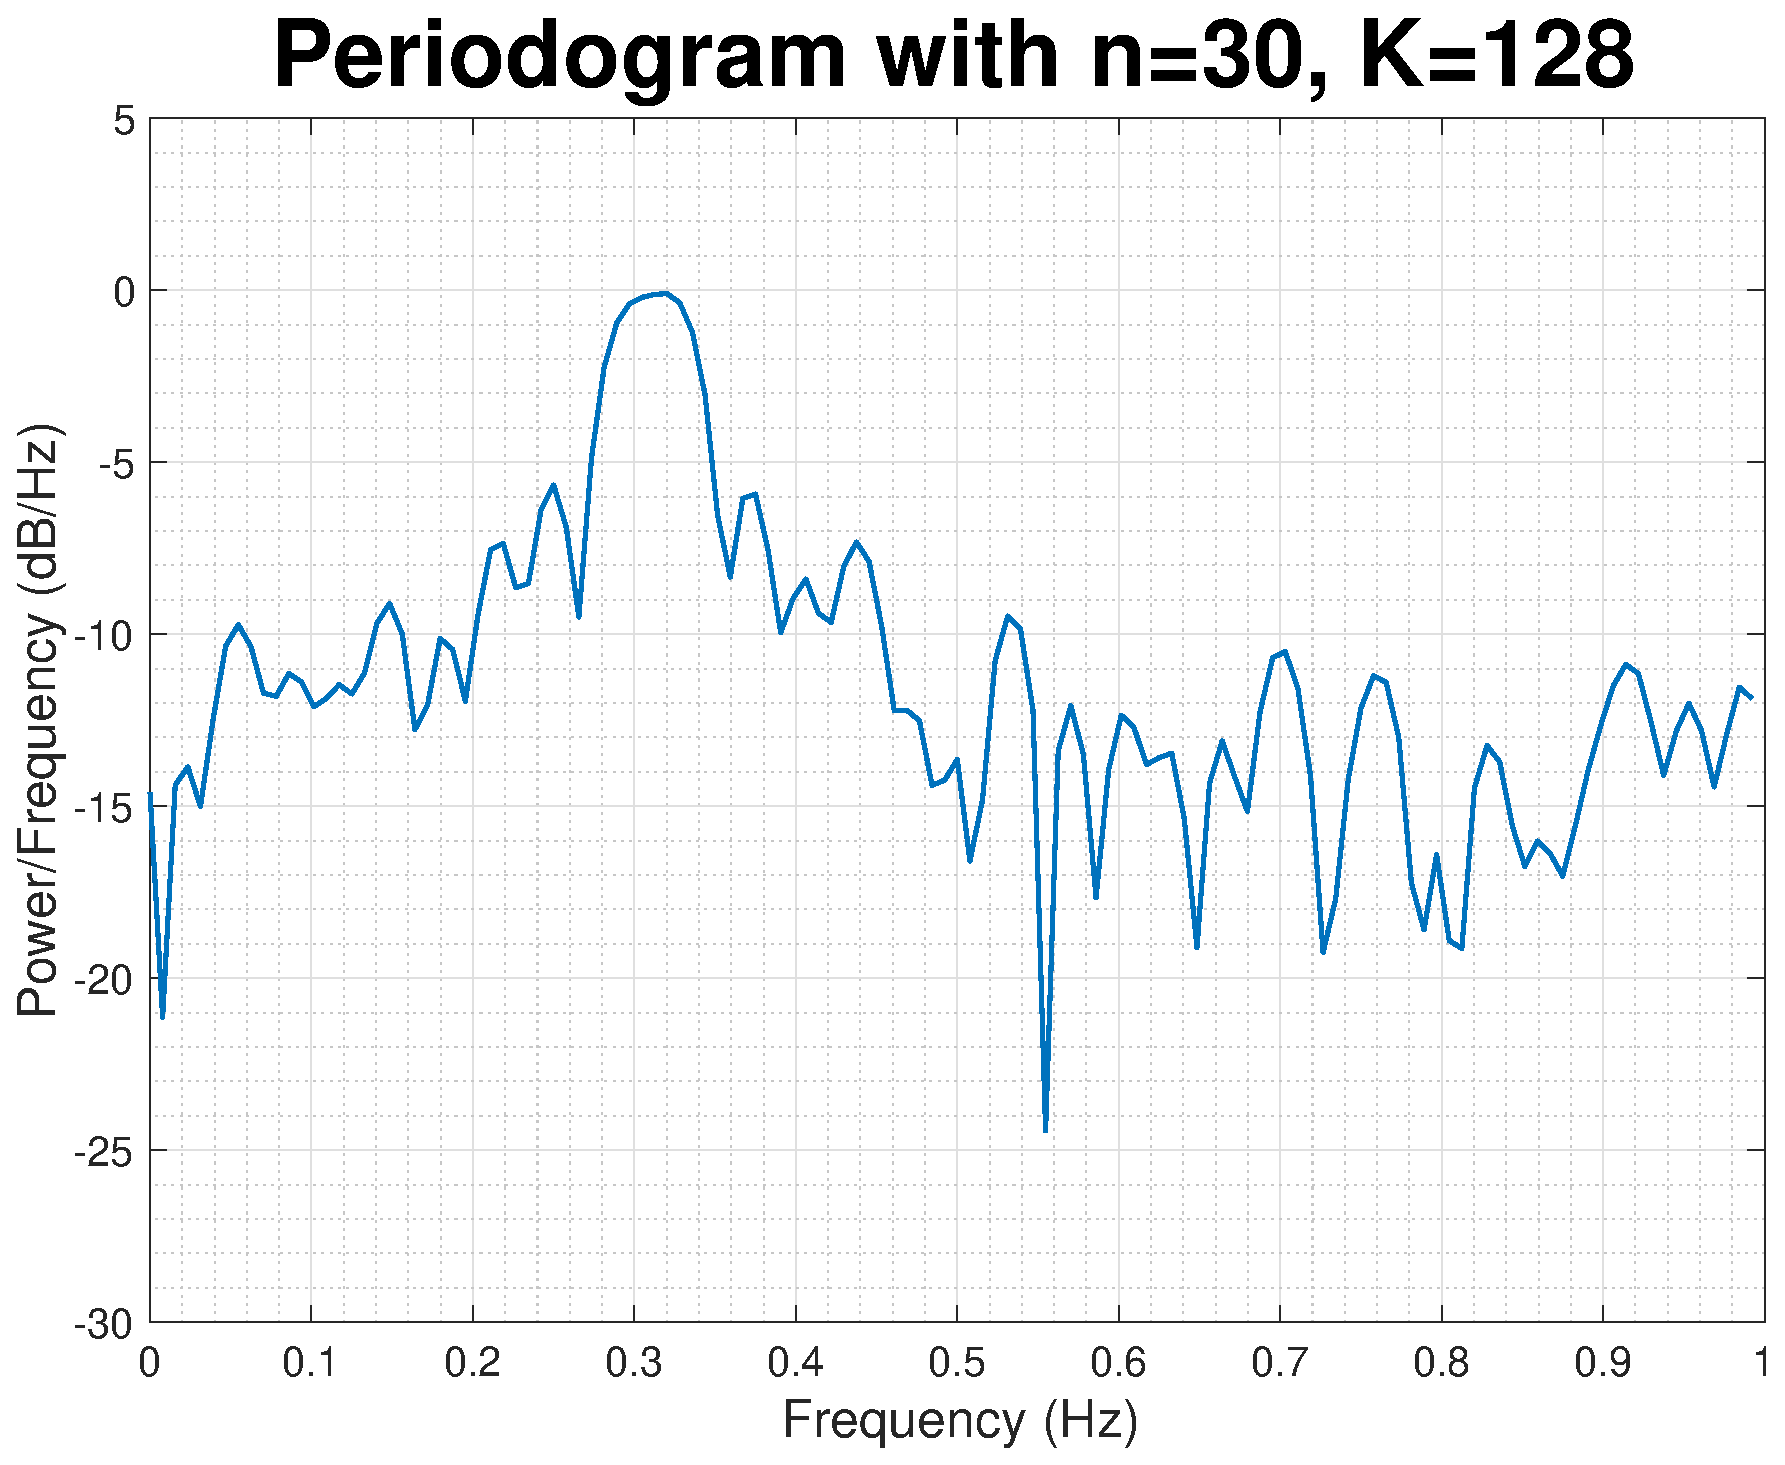
\includegraphics[width=0.32\textwidth]{part2/complex_psd_n_30}
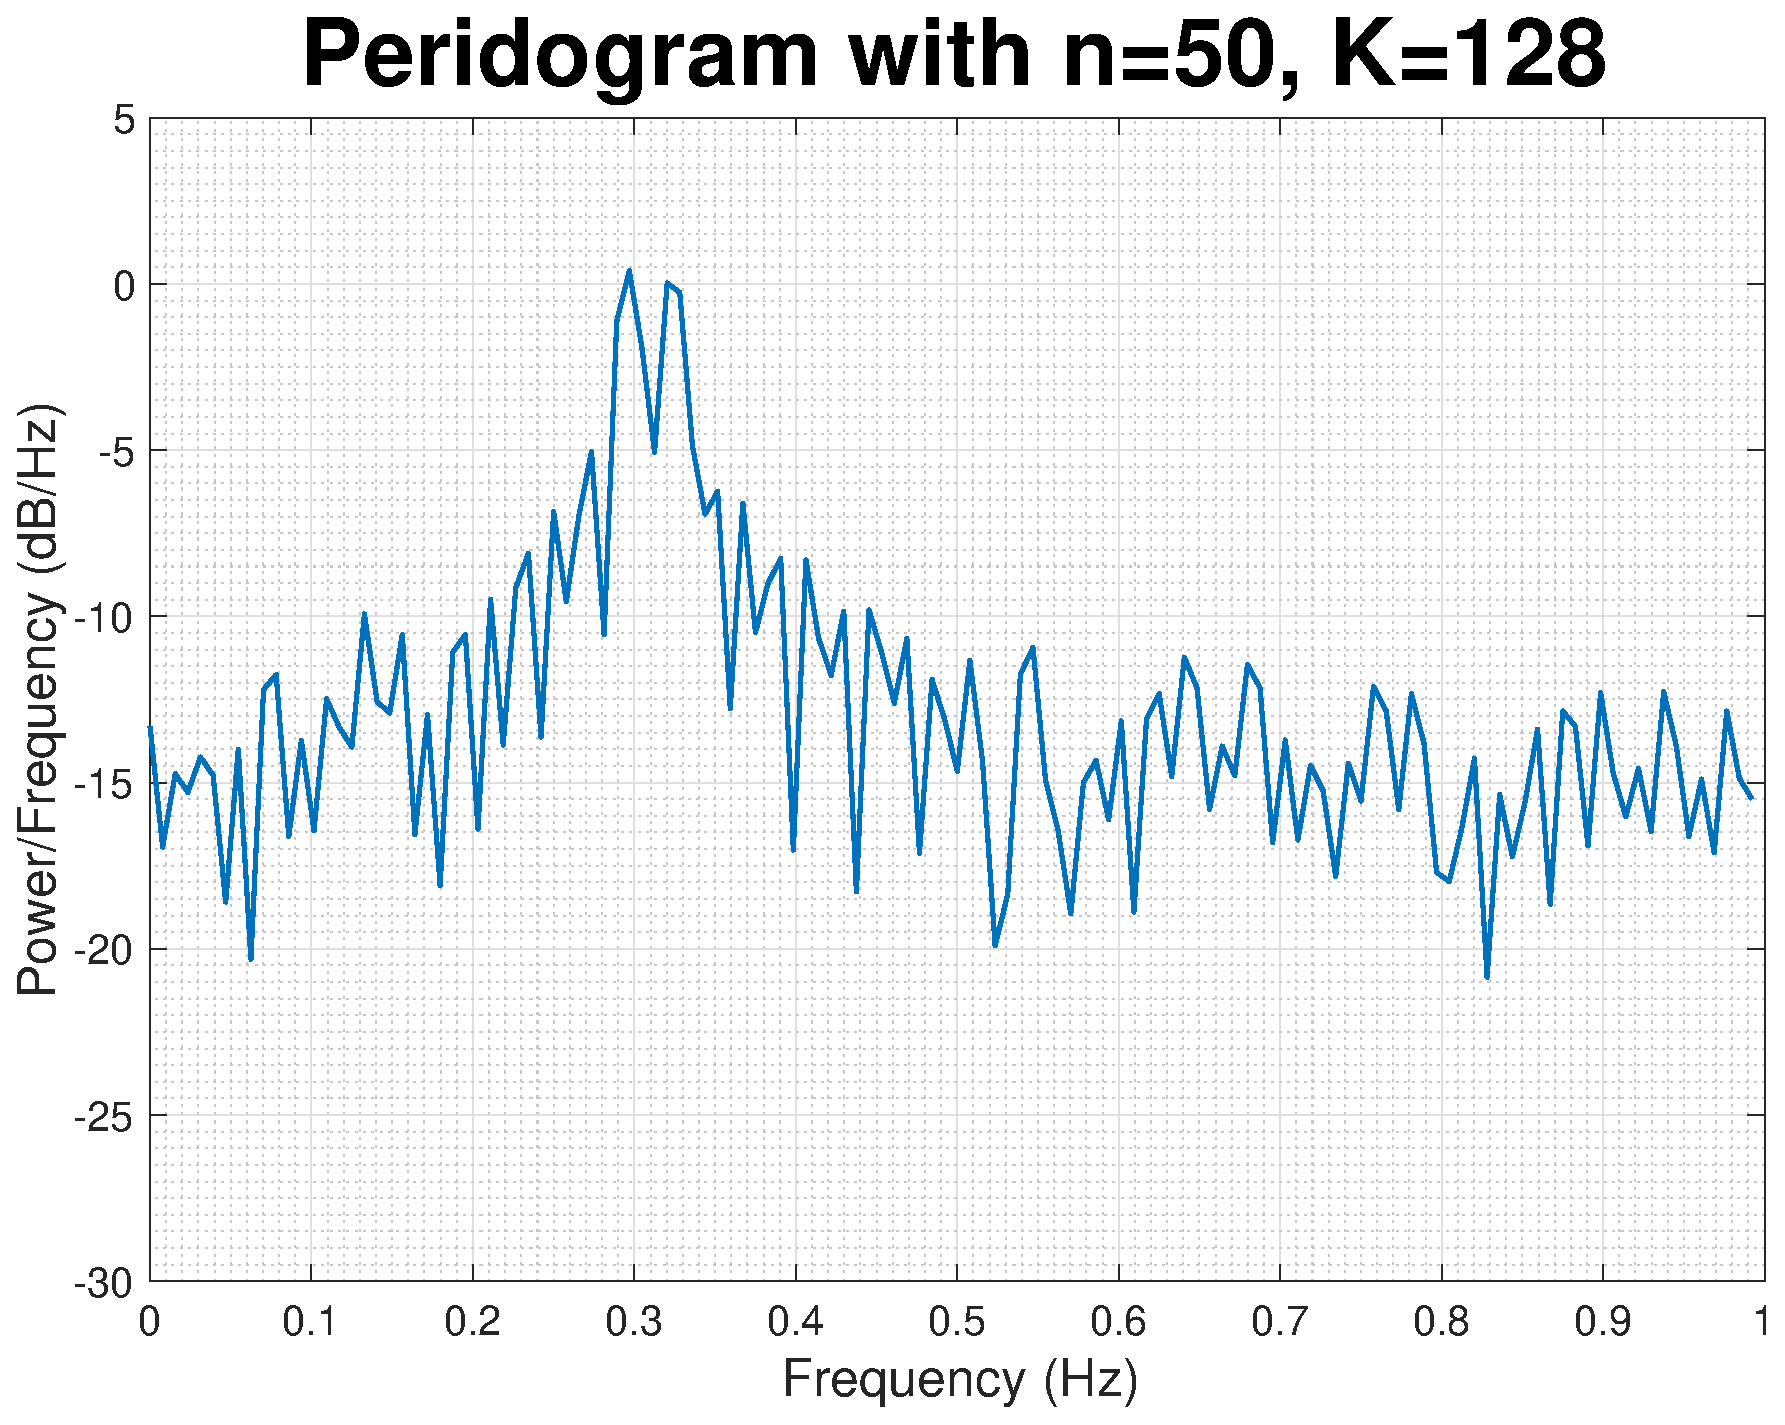
\includegraphics[width=0.32\textwidth]{part2/complex_psd_n_50}
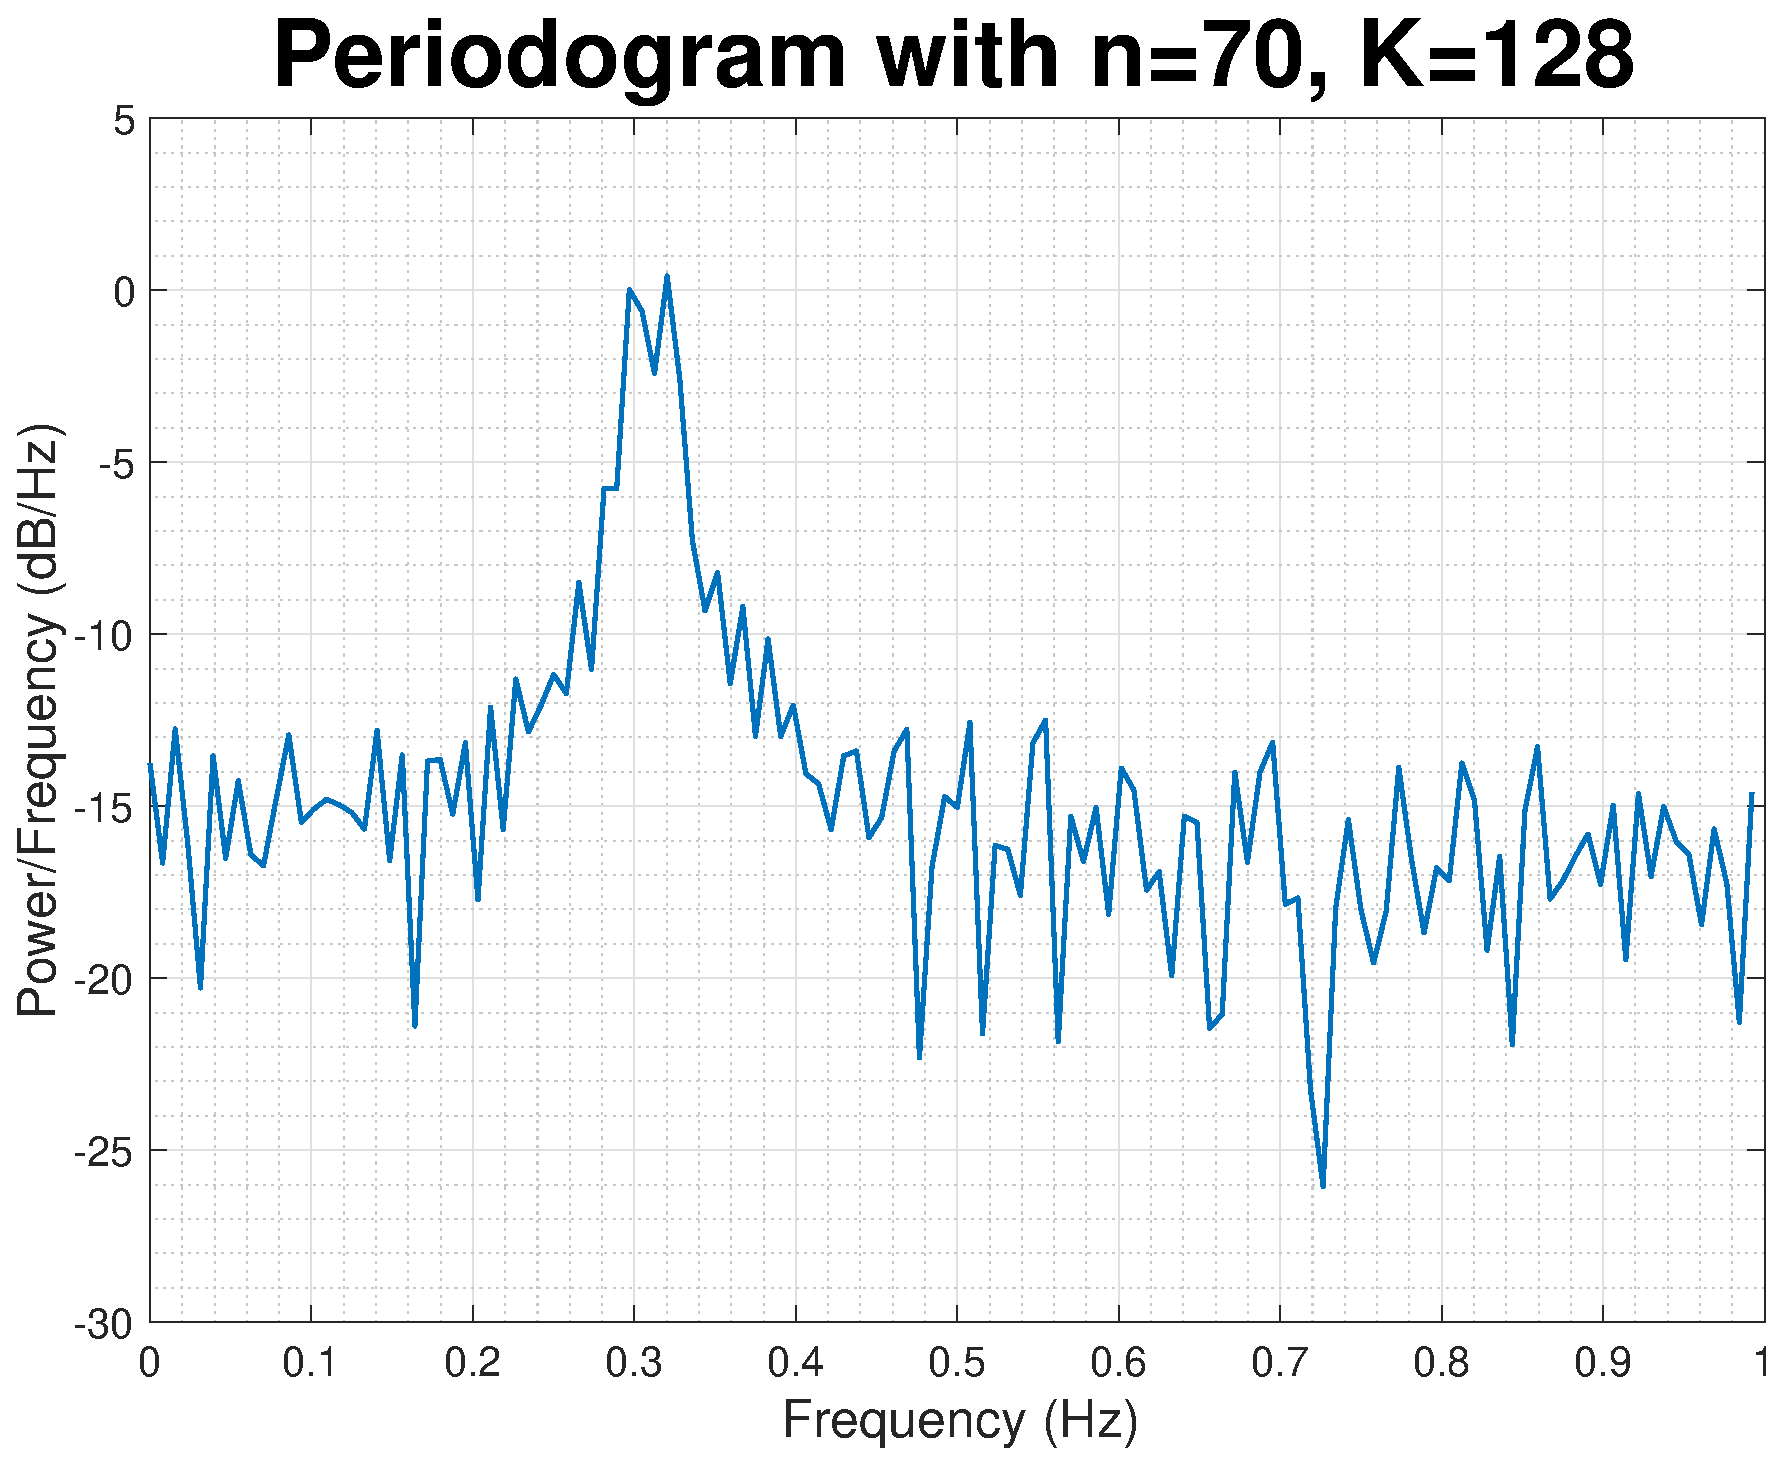
\includegraphics[width=0.32\textwidth]{part2/complex_psd_n_70}
\caption{Effect of Increasing Number of Samples on the Resolution of Periodogram Spectral Estimate}
\label{fig:complex_periodogram}
\end{figure}

\noindent{}e. The MUtiple SIgnal Classification method (MUSIC) is a frequency estimation technique that models the ACF matrix $\textbf{R}_{xx}$ as the sum of 2 ACF matrices, namely the signal ACF matrix $\textbf{R}_s$ and the noise ACF matrix $\textbf{R}_n$. The signal is assumed to be of the following form:

\begin{equation}
x(n) = A_1 e^{jn\omega_1} + w(n)
\end{equation}

Since the matrix $\textbf{R}_{xx}$ is Hermitian, the eigenvectors of the matrix are orthogonal. As such, the following equation is true, where $e_{i}$ is a eigenvector from matrix $\textbf{R}_s$ whereas $v$ is an eigenvector from $\textbf{R}_n$ and $\textbf{R}_{xx}$ is an $MxM$ matrix and there are $p$ complex exponentials present in the signal:

\begin{equation}
\textbf{e}_{i}^H \textbf{v} = \sum_{k=0}^{M-1} v(k)e%^{-jk\omega_{i}} = 0; i=1,2,\dots,p
\end{equation}

\noindent{}The power spectrum as be estimated using the following formula, where $\textbf{e} = [1, e^{j\omega}, e^{j2\omega},\dots, e^{j(M-1)\omega}]$. Note that a discrete-time signal has a finite set of unique complex exponentials that are all contained with the vector $\textbf{e}$. This is due to the fact that the complex exponentials are periodic and this forms the basis of the Discrete Fourier Transform:

\begin{equation}
\hat{P}_{MU}(e^{j\omega}) = \frac{1}{\sum_{i=p+1}^M|\textbf{e}^H v_{i}|^2}
\end{equation}

\noindent{}Since the eigenvectors $\textbf{e}$ and $v_{i}$ are orthogonal, the inner product should have $p$ roots which lie on the unit circle and correspond to the frequencies of the complex exponentials that are present in the signal. However, since the matrix $\textbf{R}_{xx}$ is $MxM$ where $M > p + 1$, then the inner product will have $M-p-1$ zeros which lie anywhere on the z-plane. In fact, the zeroes could lie very close to the unit circle and thus lead to suprious peaks in the power spectrum that could be mistaken as a complex exponentials that is present within the signal. To reduce the likelihood of this occuring, we average the estimate using all of the $M-p-1$ eigenvectors corresponding to the noise. The averaging effect will amplify the magnitude of the true peaks and thus makes identifying complex exponentials that are actually present within our signal more accurate. \\

\noindent{}Having understood how the algorithm works, it is clear that the first line gives the ACF matrix $R$ that has the dimensions $MxM$, where $M=14$. This value of $M$ is selected based on the fact that we can only trust that many ACF values. Larger values of $M$ could be selected however, as seen above, as the lag increases, the accuracy with which ACF estimation can be performed decreases. The second line of the code performs the spectral estimation using the MUSIC algorithm. The ACF matrix is provided as the first argument while the dimension of the signal subspace $p$, is given as the second argument. The third are fourth arguments are related to the length of the FFT and the sampling period while the last argument informs the function to treat the first argument as a correlation matrix rather than a data matrix. 

\begin{figure}[H]
\centering{}
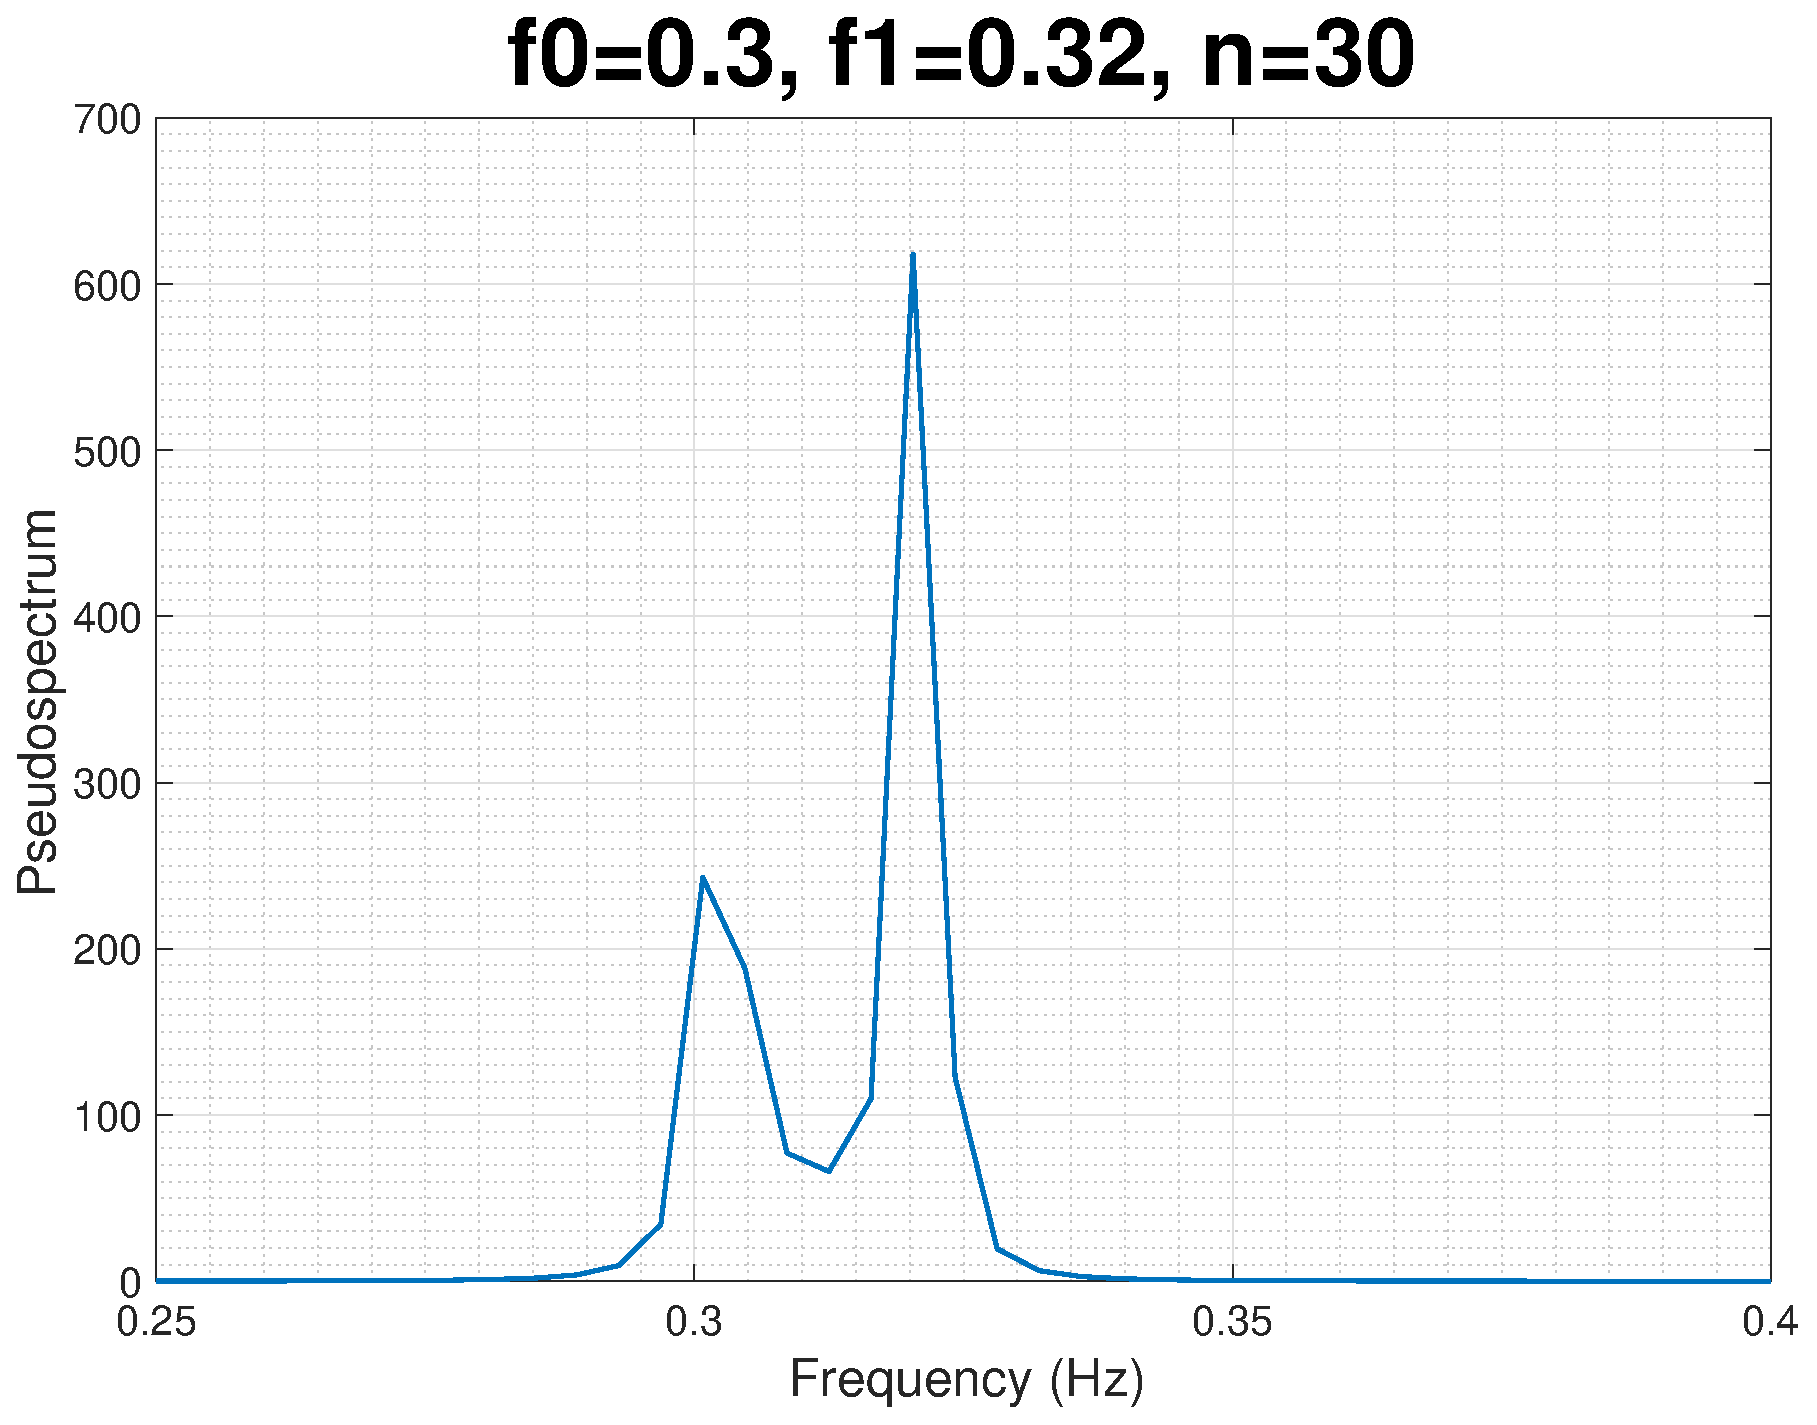
\includegraphics[width=0.32\textwidth]{part2/music_2_sinewaves_n_30}
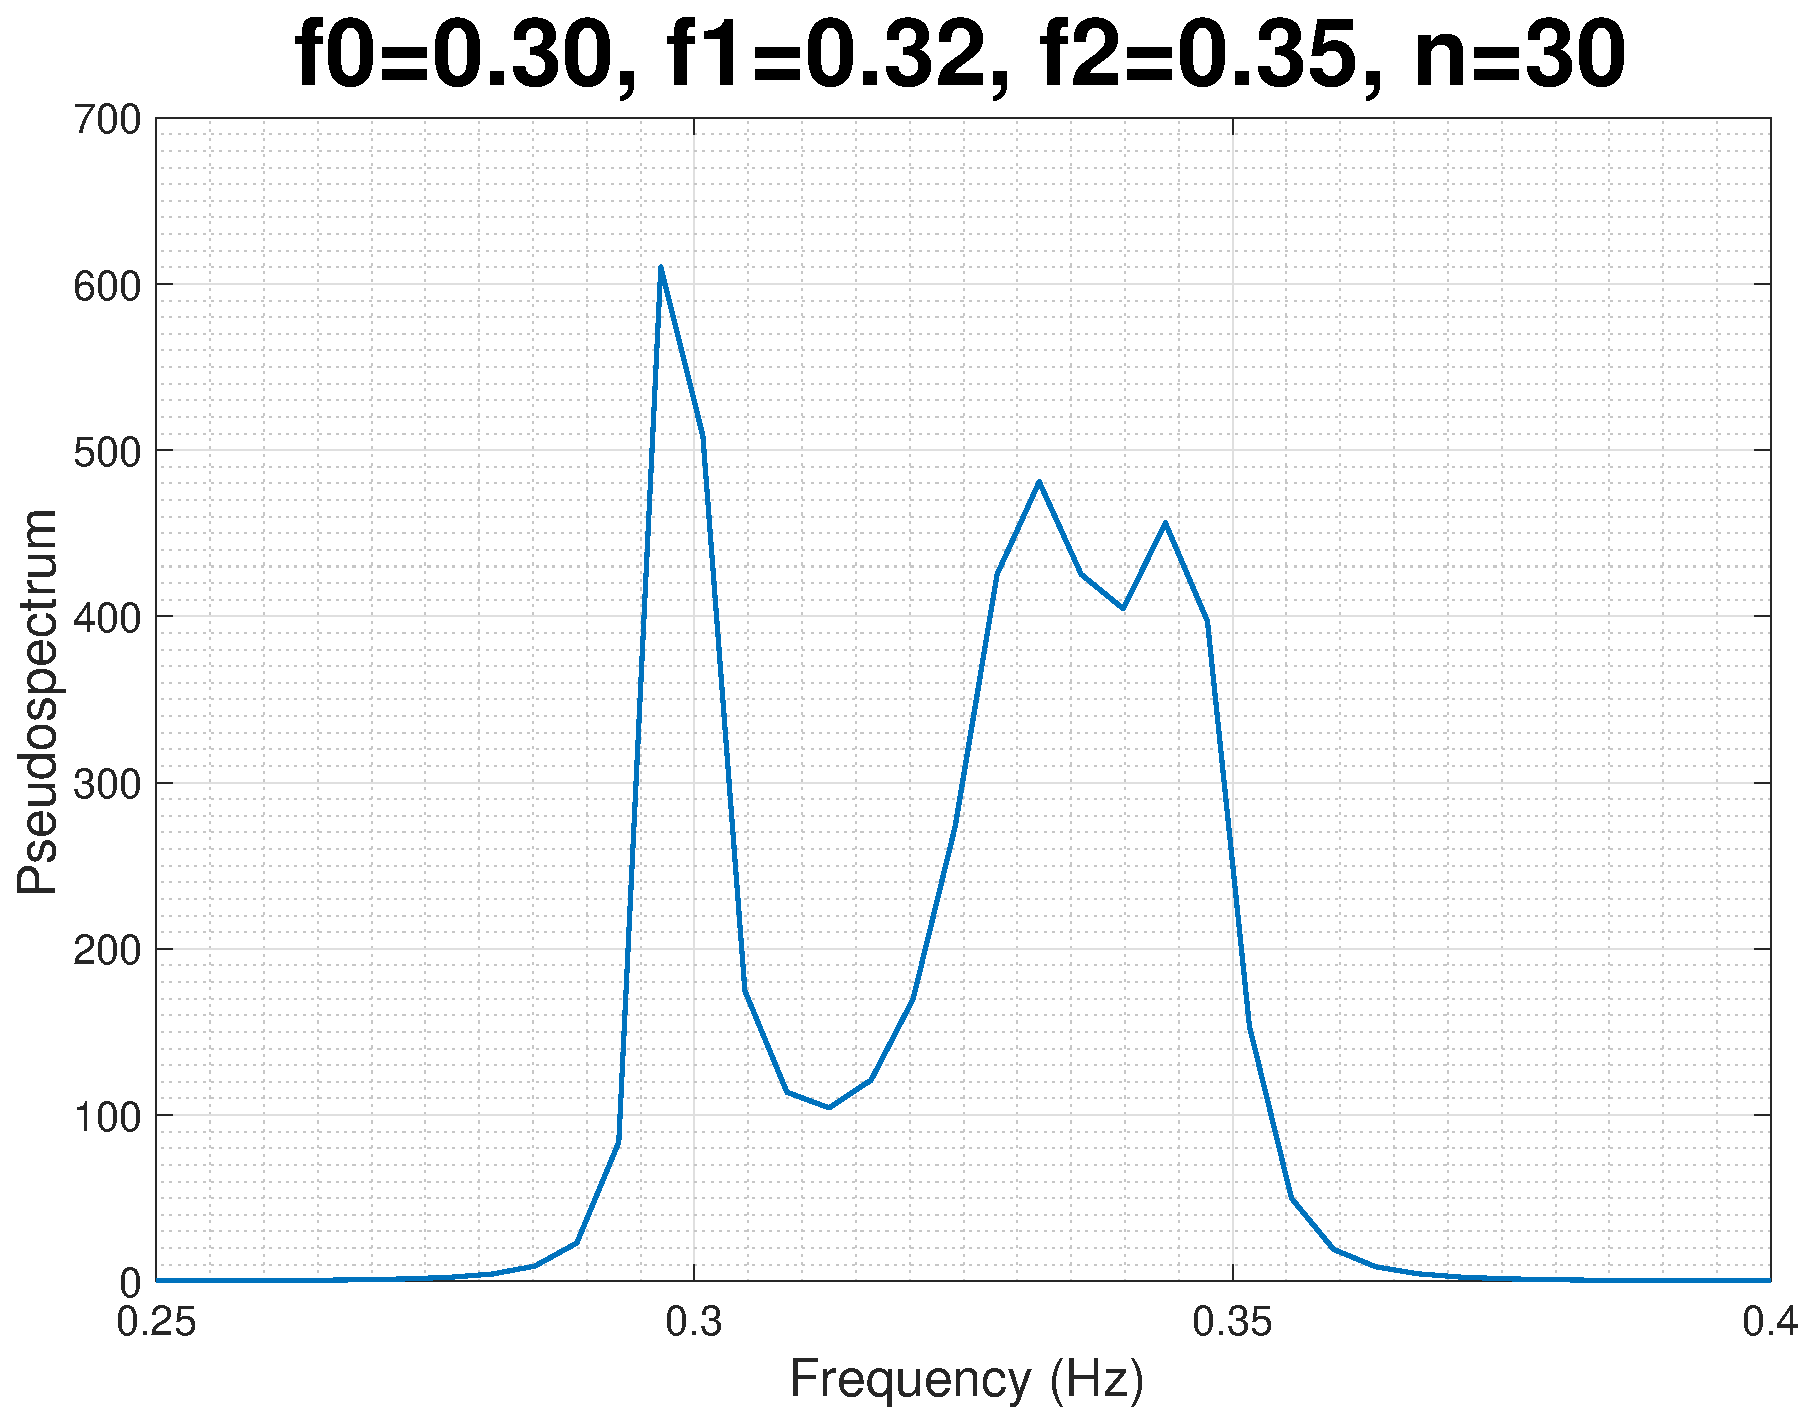
\includegraphics[width=0.32\textwidth]{part2/music_3_sine_waves_n_30}
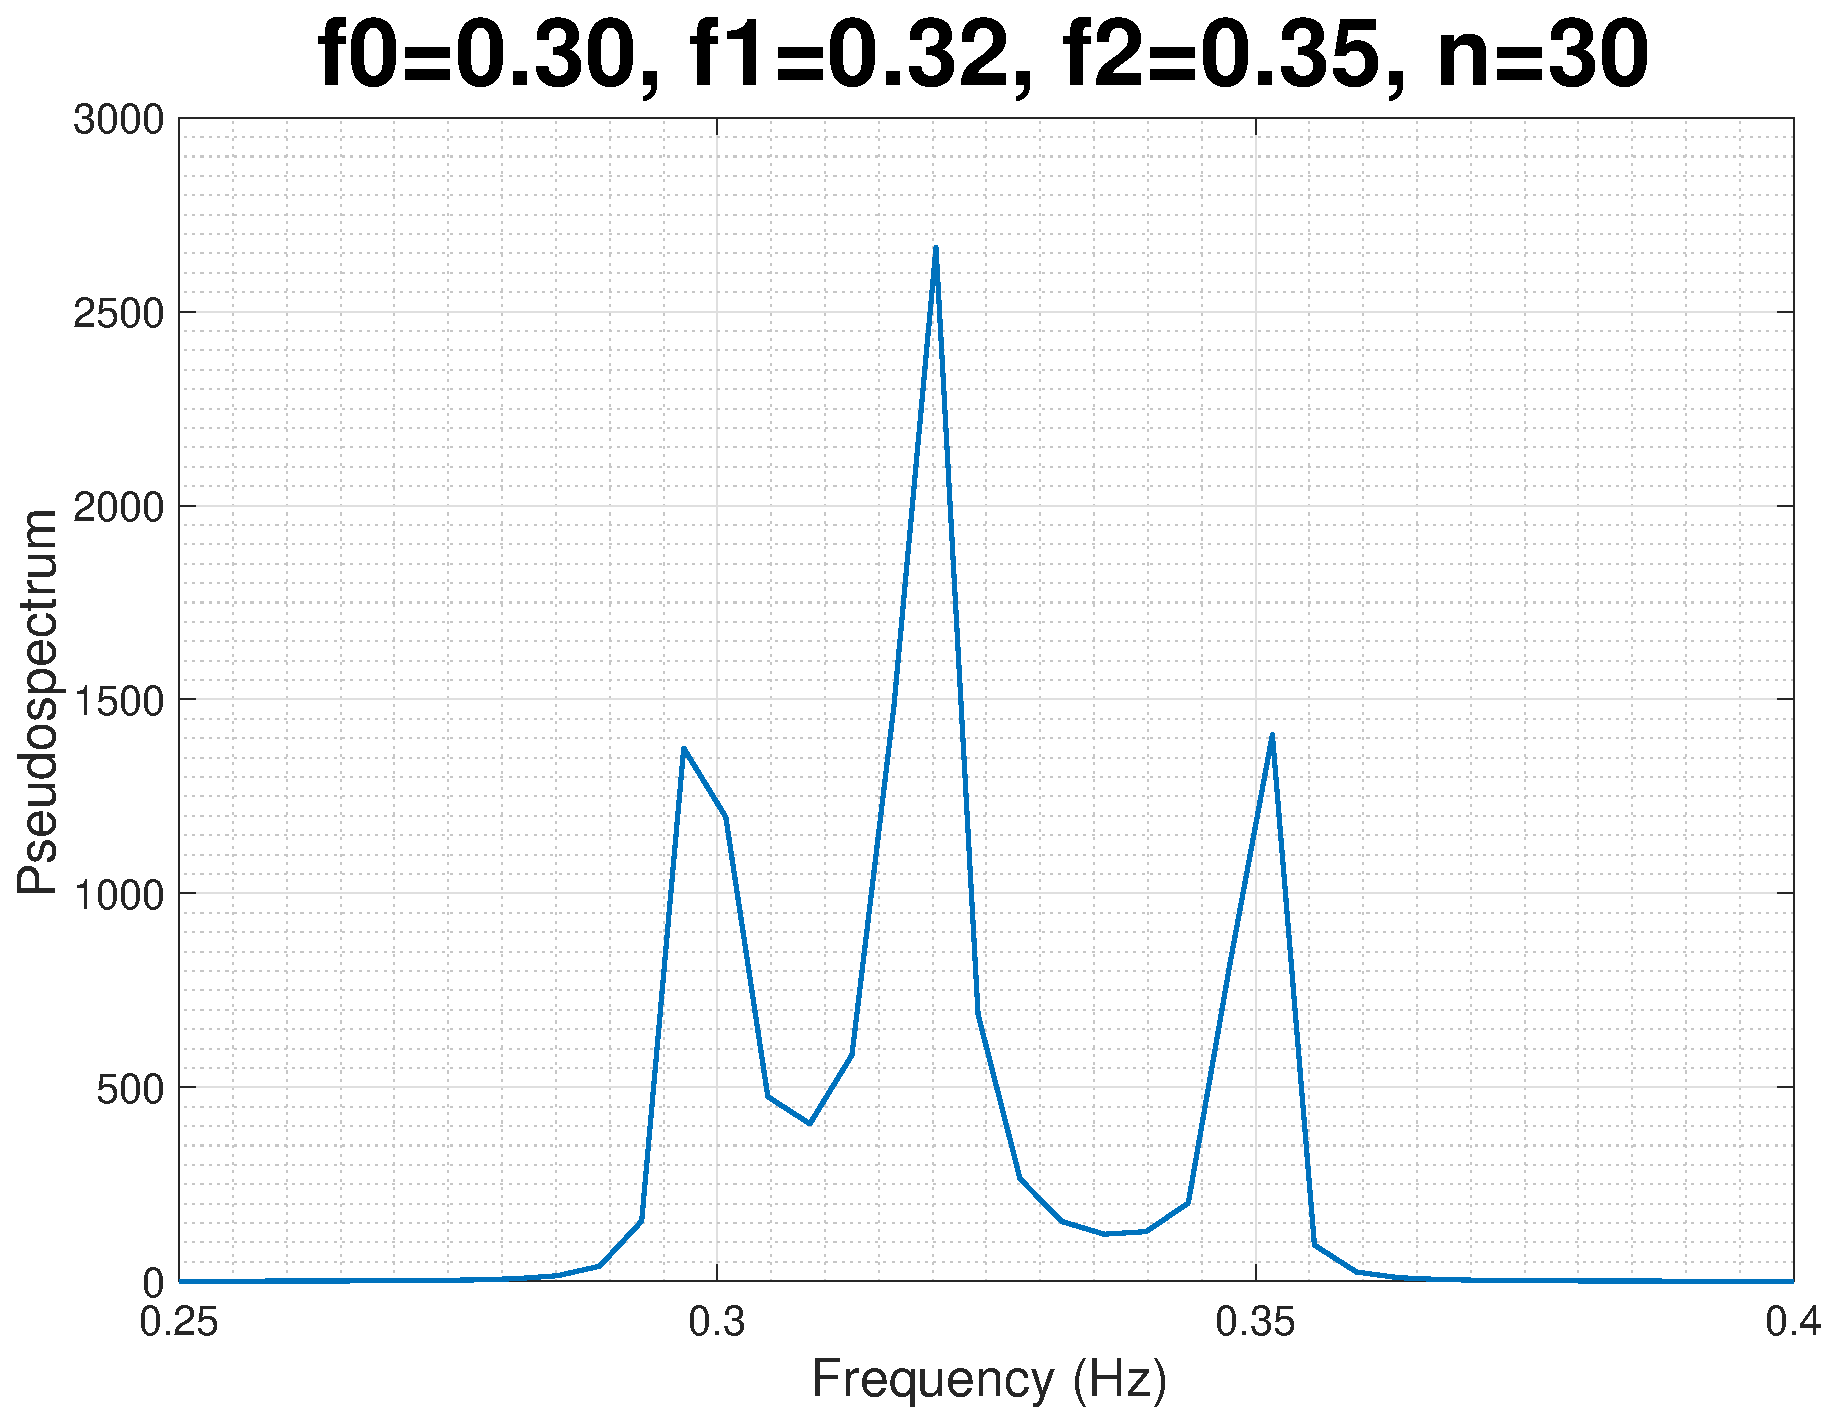
\includegraphics[width=0.32\textwidth]{part2/music_3_sine_waves_n_70}
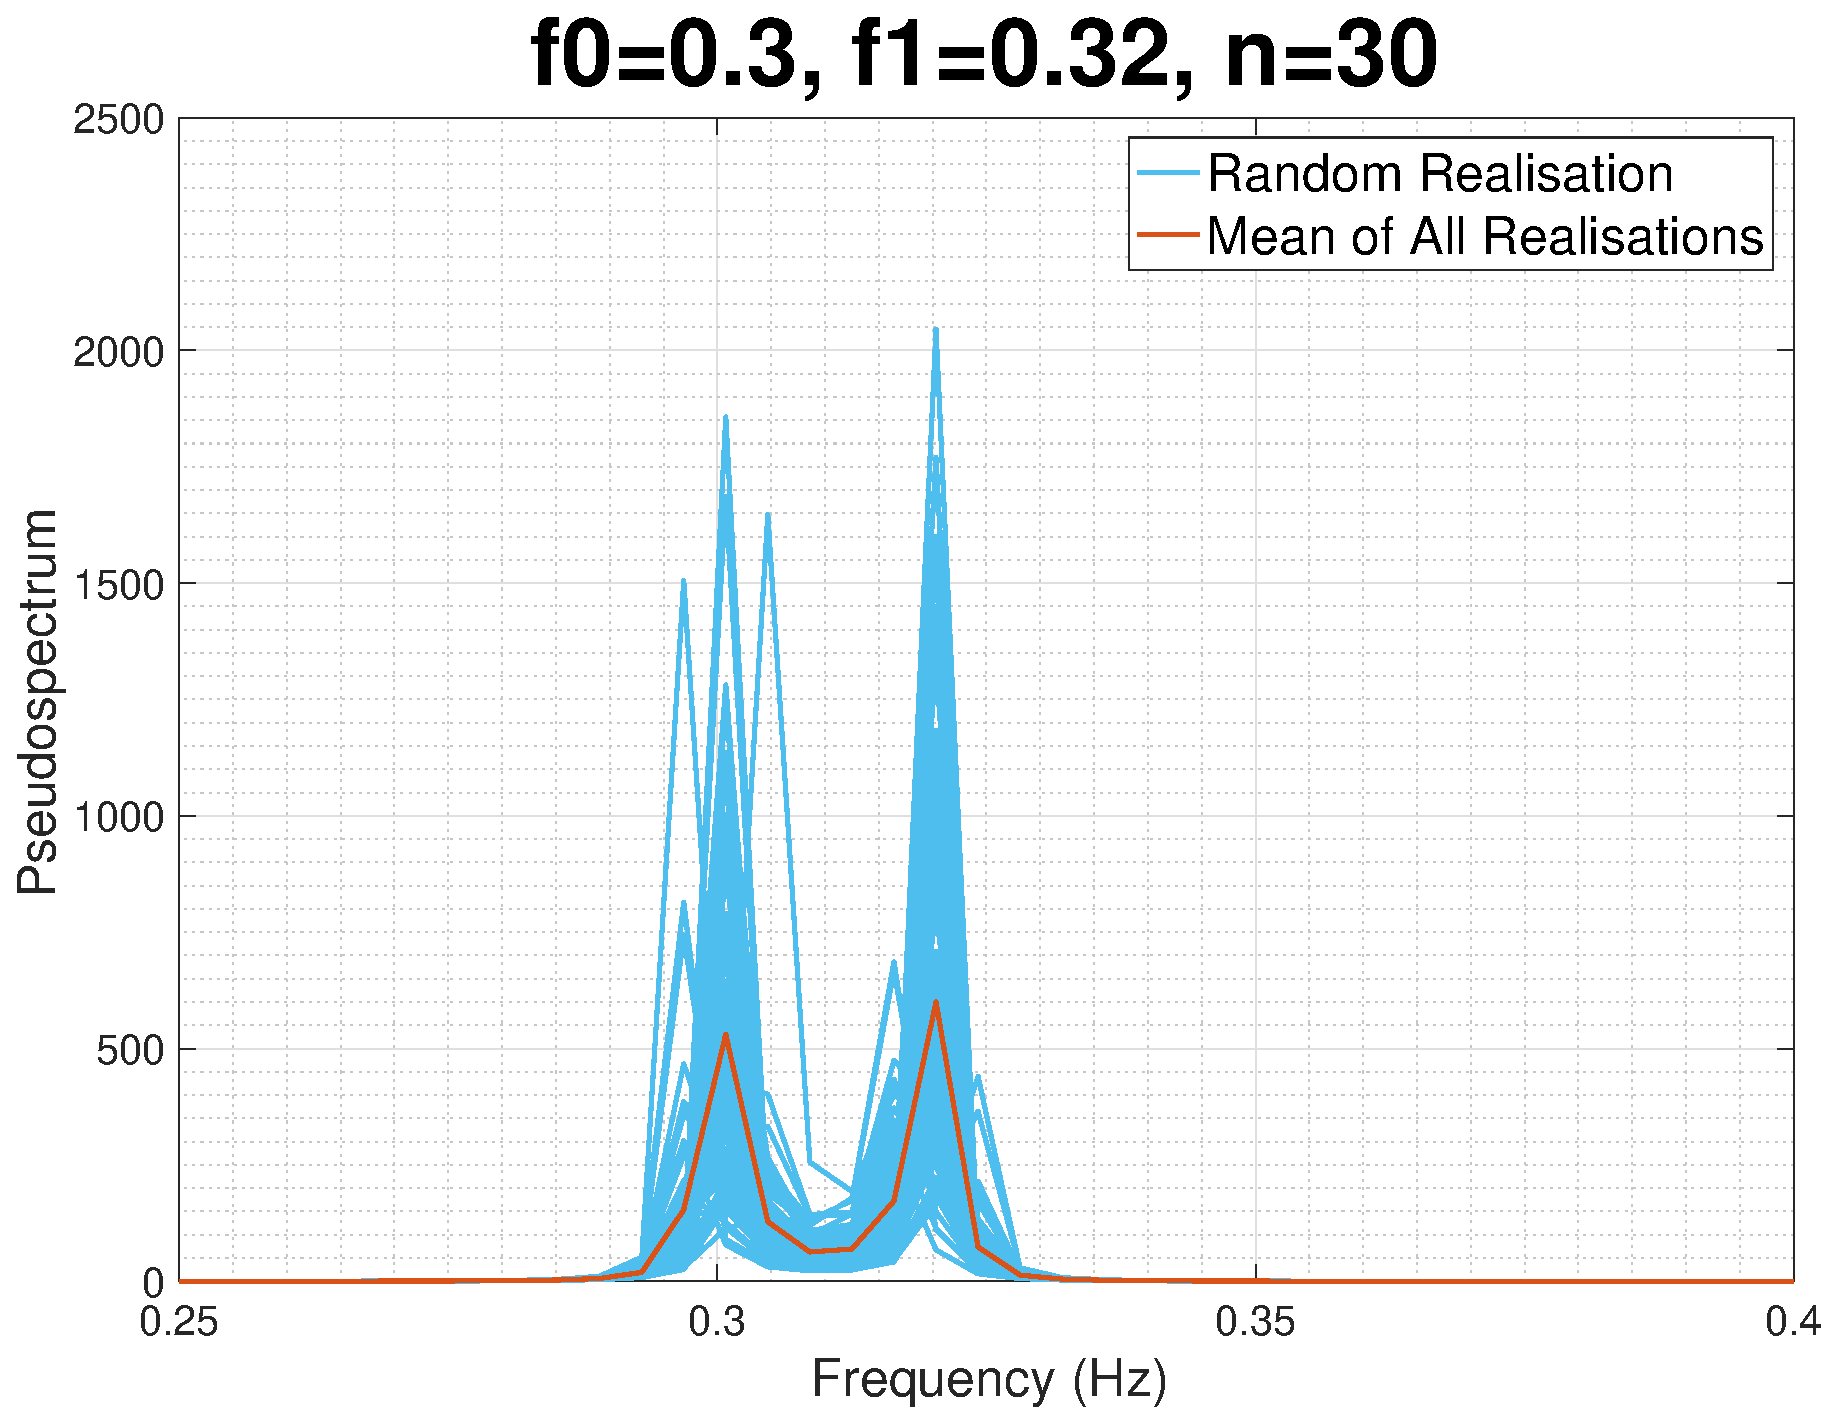
\includegraphics[width=0.32\textwidth]{part2/music_2_sinewaves_n_30_overlay}
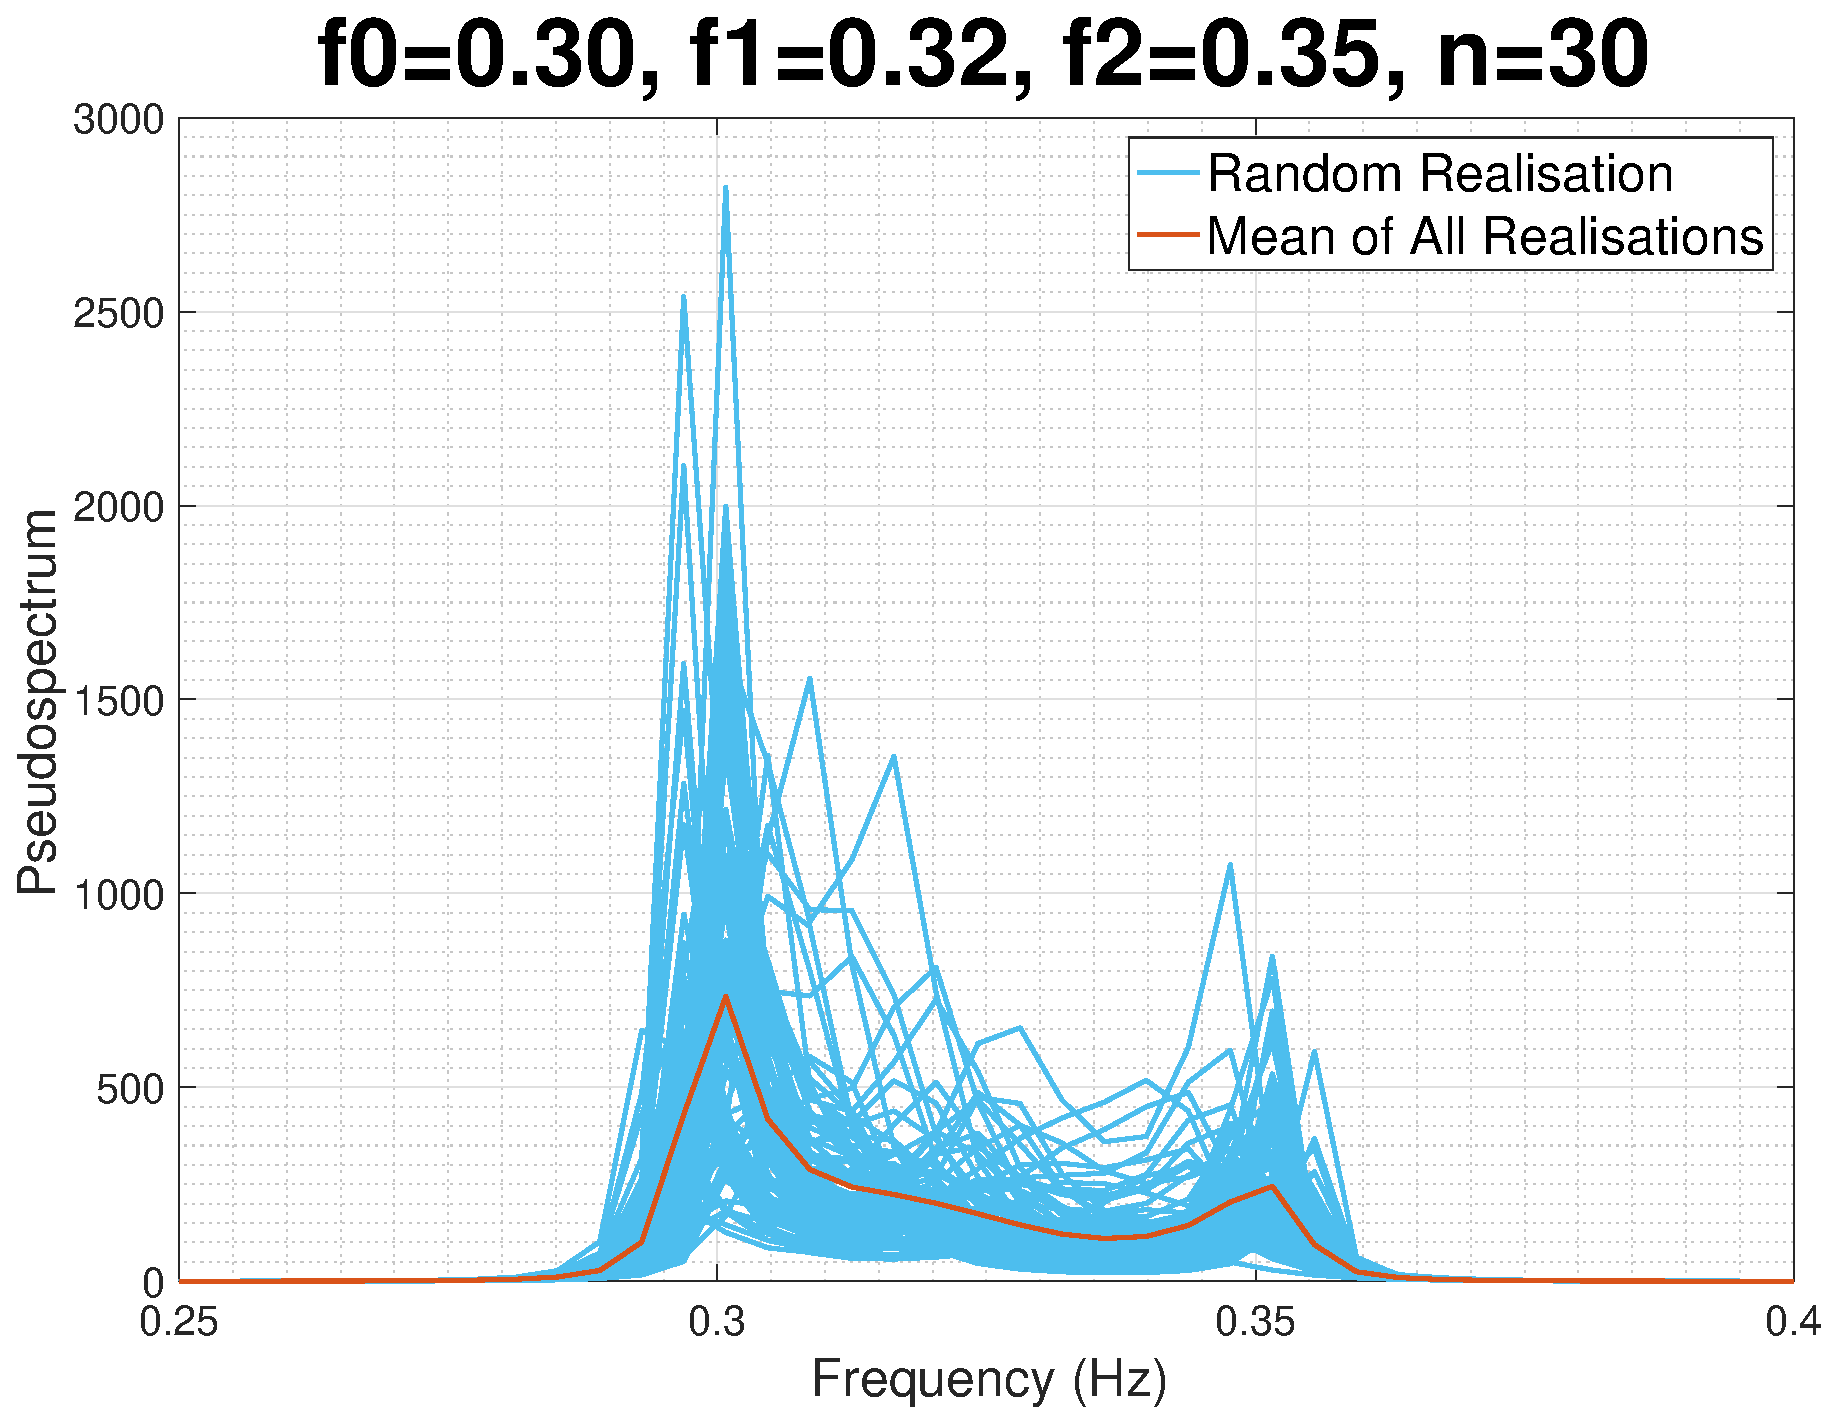
\includegraphics[width=0.32\textwidth]{part2/music_3_sinewaves_n_30_overlay}
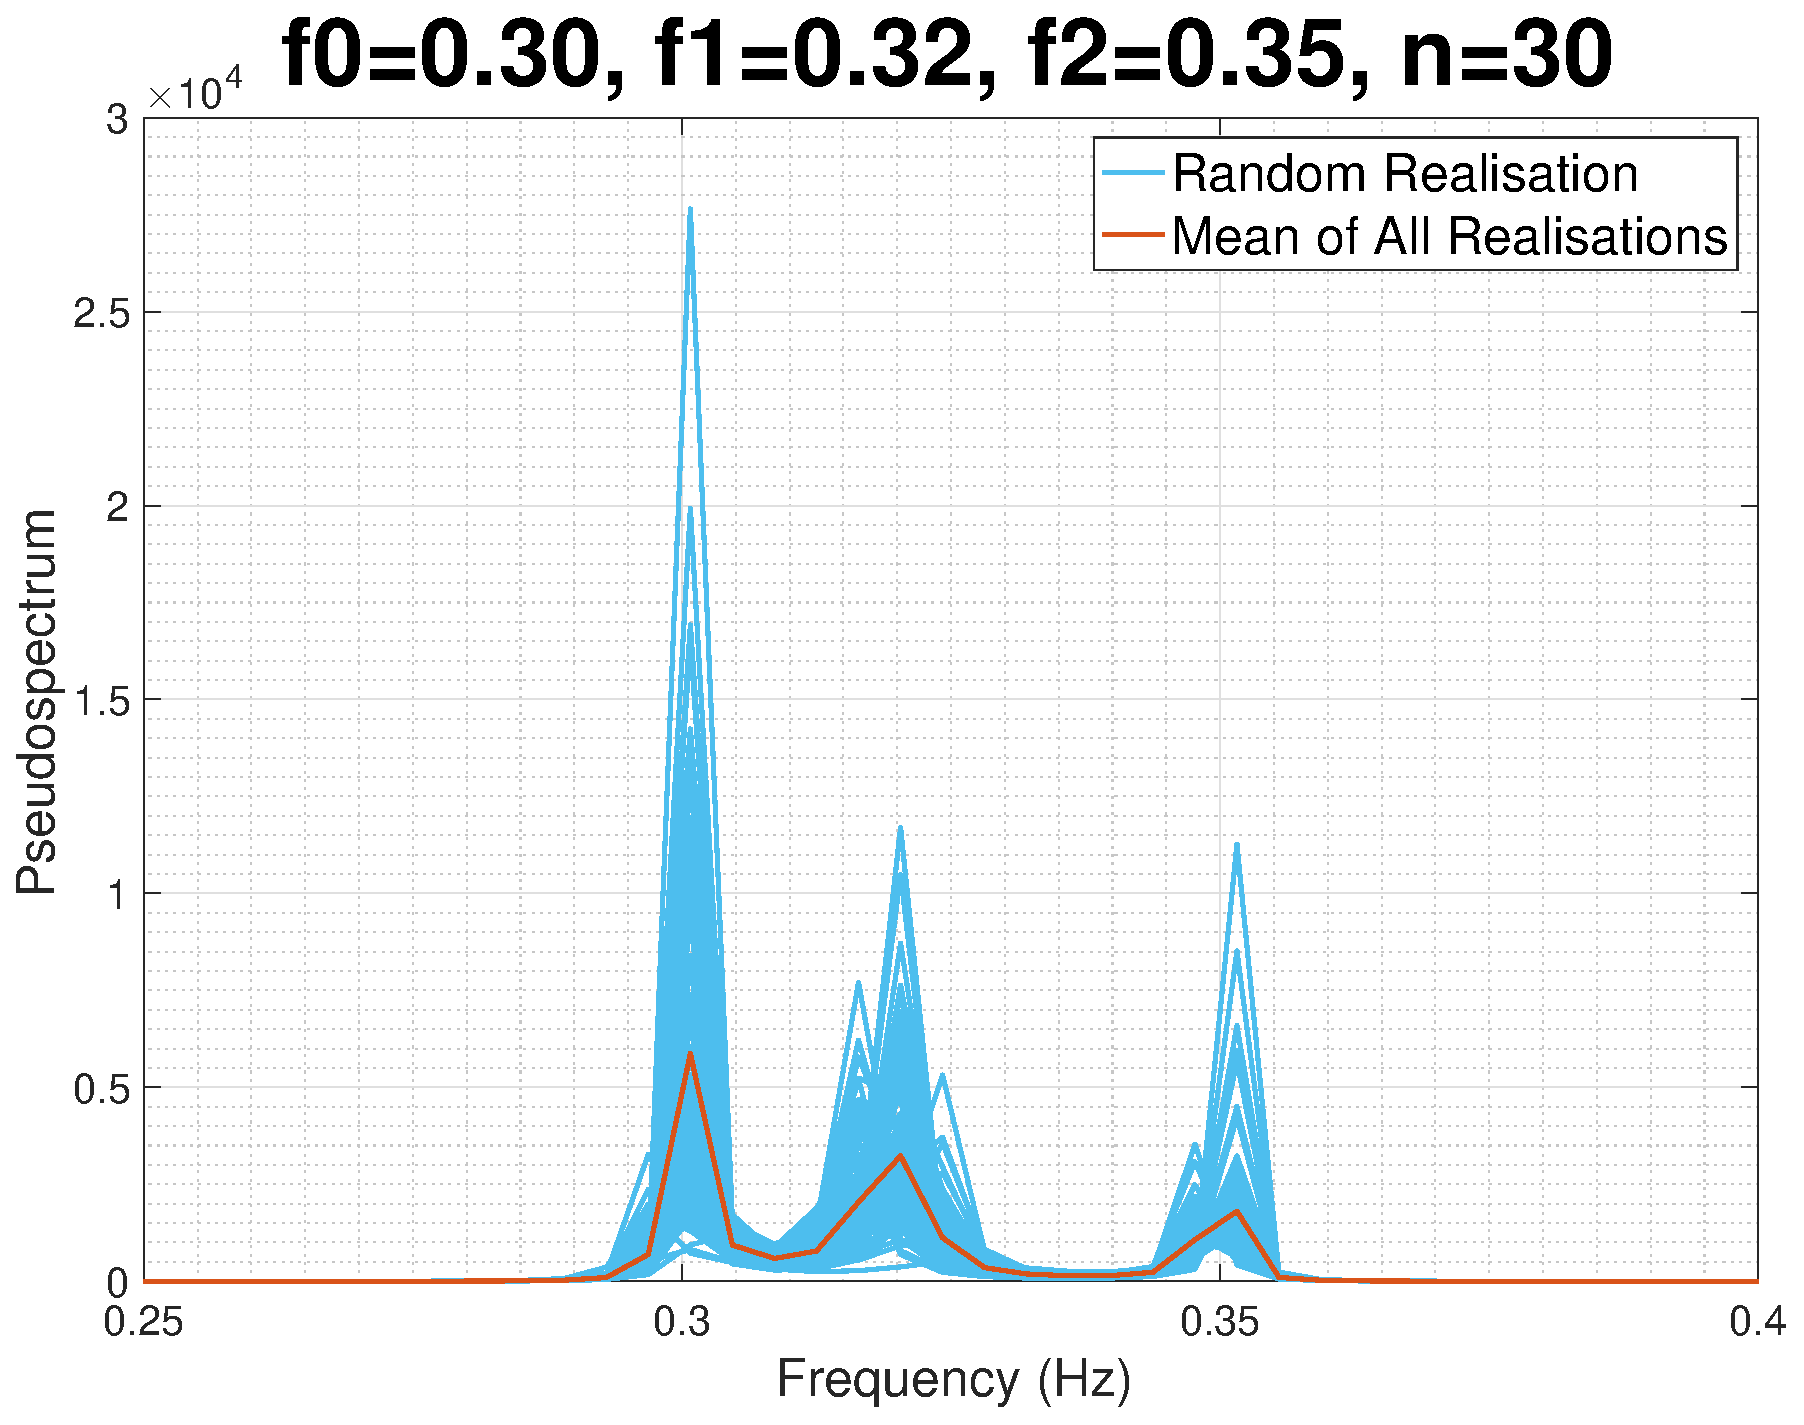
\includegraphics[width=0.32\textwidth]{part2/music_3_sinewaves_n_70_overlay}
\caption{Detecting Sinewaves using MUSIC, and Effect of Increasing Number of Samples on the Resolution of Estimate}
\label{fig:music}
\end{figure}

\noindent{}The figures above shows the results obtained. The first row shows just one realisation of the random signal $x$, whereas the second row shows an overlay of 100 realisations. It is clear that the MUSIC algorithm, like the periodogram has a frequency resolution limit as it is not able to identify 3 sinewaves that are very closely spaced together. However increasing the number of samples, like for the periodogram, increases the frequency resolution and distinguishing the sinewaves is now possible.\\

\noindent{}The main advantage of the MUSIC algorithm is the ability to identify complex exponentials when very few samples are available. This is clear when comparing the results obtained in Figure \ref{fig:music} to those obtained in Figure \ref{fig:complex_periodogram}. The disadvantages are that the pseudospectrum does not provide information about the magnitude of the complex exponentials. Notice that the signal $x$ was generated with equal magnitudes for each of the complex exponentials but the pseudospectrum did not highlight this. Secondly, the algorithm requires, as an input, the dimensionality of the signal subspace. Often, this may not be known. Lastly, the averaging that is performed to remove spurious peaks from the spectra have the adverse effect of removing information about the noise spectra; this information may be especially useful if the noise is non-white.


\subsection{Spectrum of Autoregrssive Processes}

\noindent{}a. Autoregressive (AR) parameter estimation is performing using the following equation:

\begin{equation*}
\textbf{r}_{xx} = \textbf{R}_{xx}a \implies a = \textbf{R}_{xx}^{-1}\textbf{r}_{xx}
\end{equation*}

\noindent{}It is just crucial that the matrix $\textbf{R}_{xx}$ is invertible. When the ACF is calculated using the biased estimator, it is guaranteed to be positive definite and thus invertible, however this is not gauranteed when the unbiased estimator is utilized.

\begin{figure}[H]
\centering{}
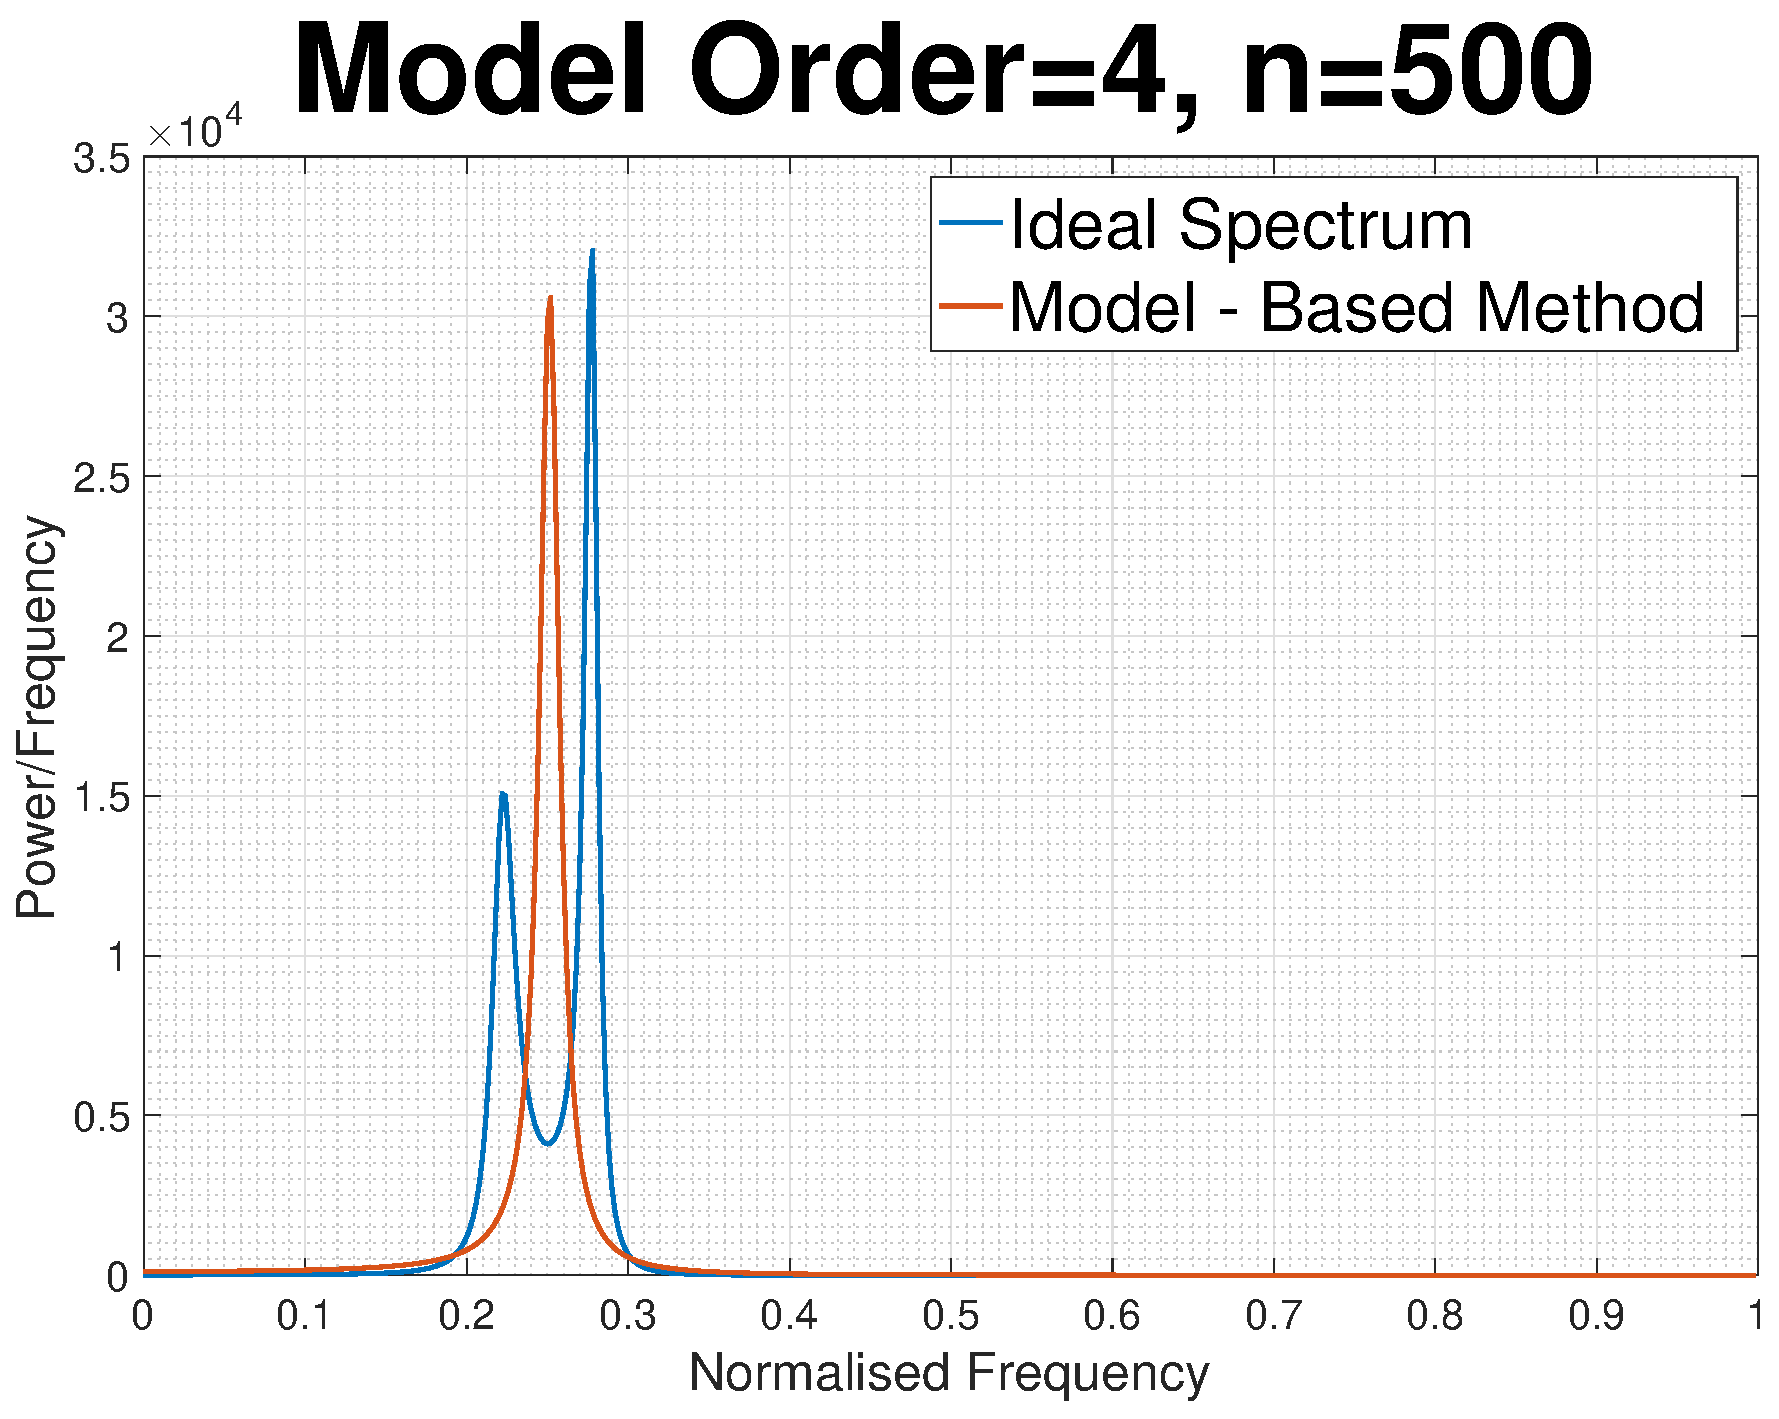
\includegraphics[width=0.24\textwidth]{part2/ar_spectrum_estimate_order_4}
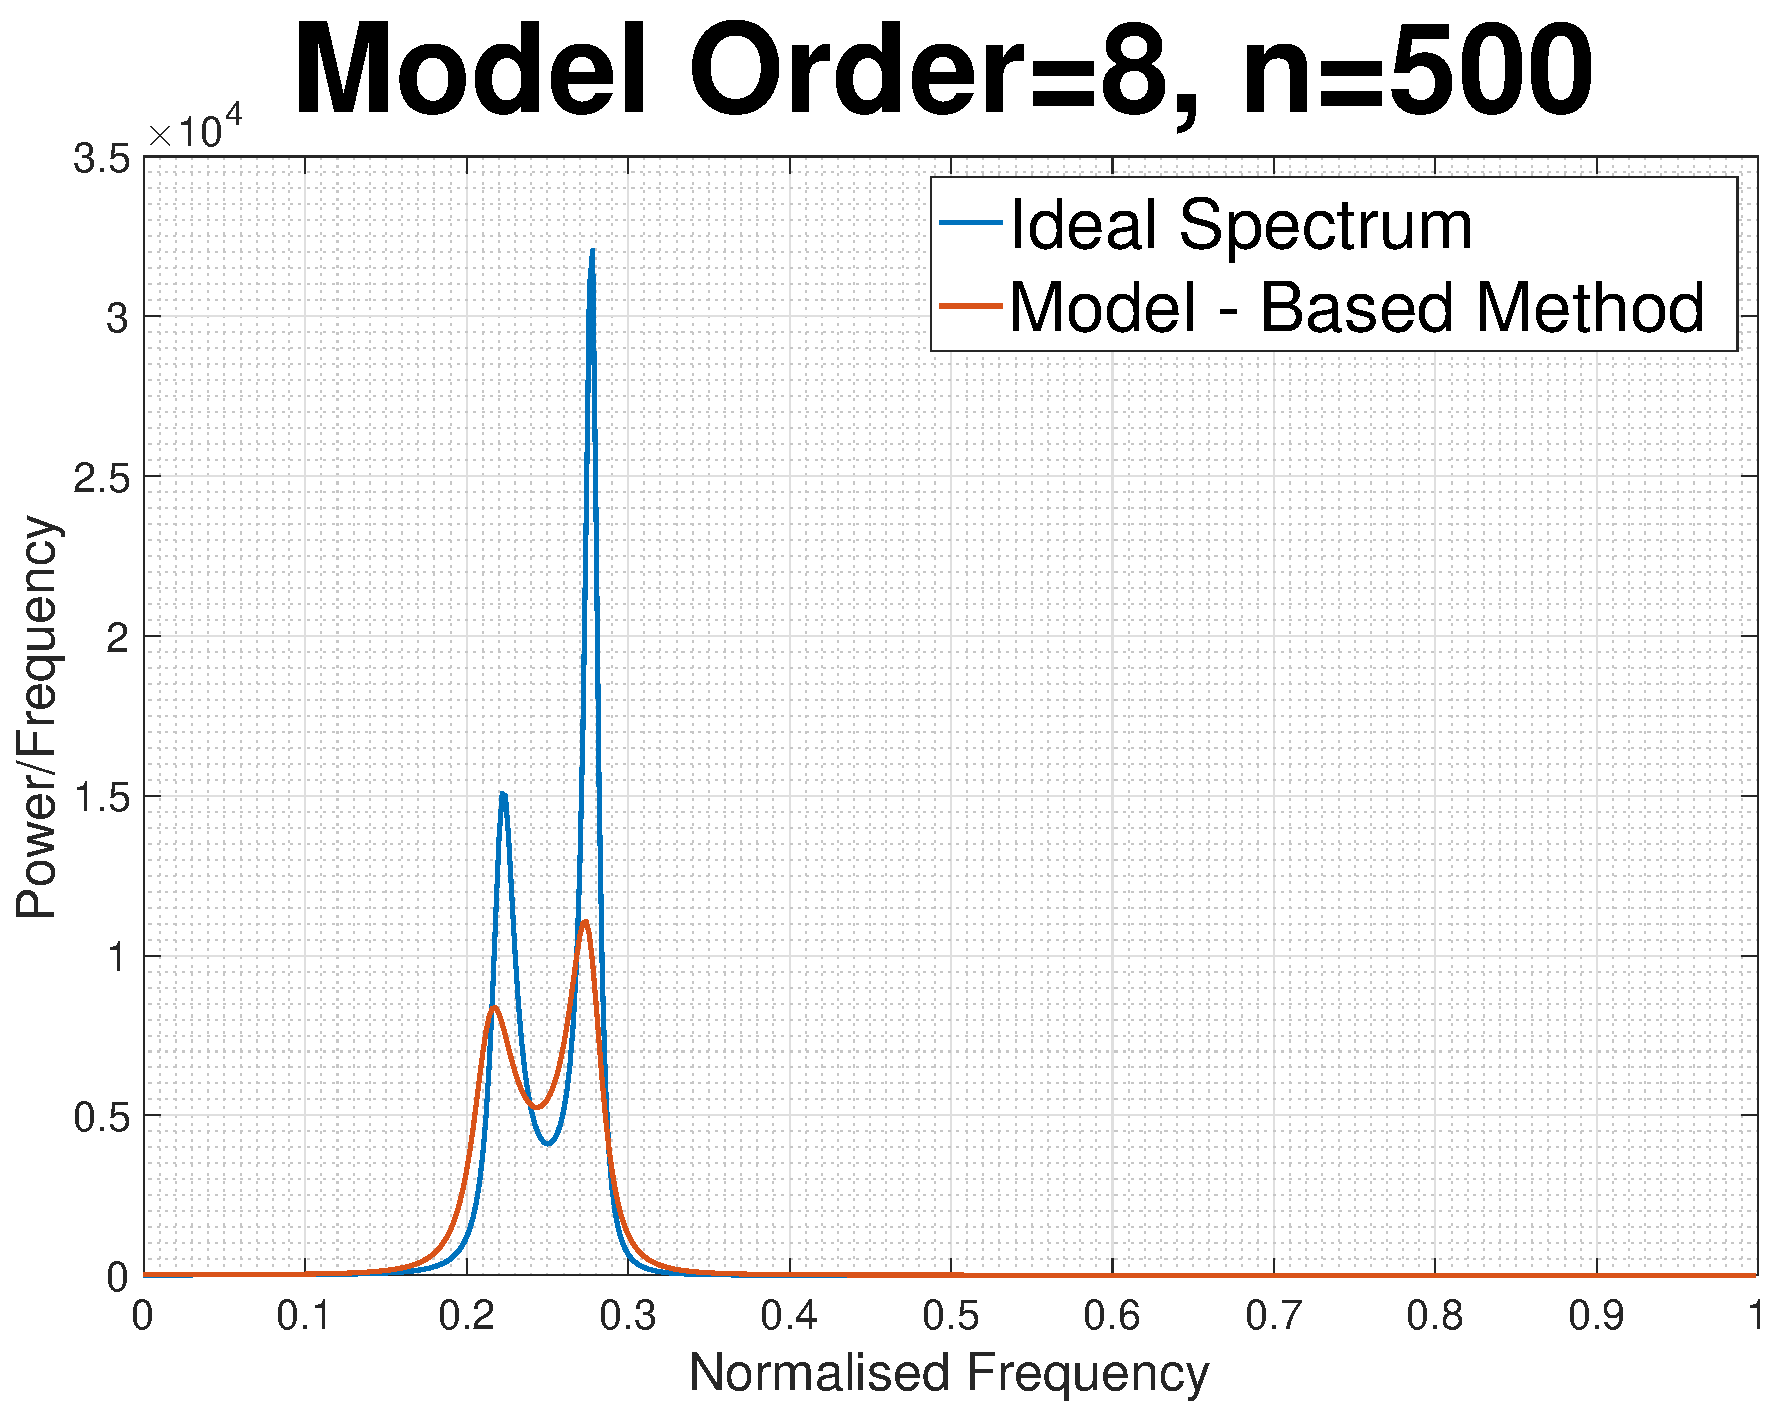
\includegraphics[width=0.24\textwidth]{part2/ar_spectrum_estimate_order_8}
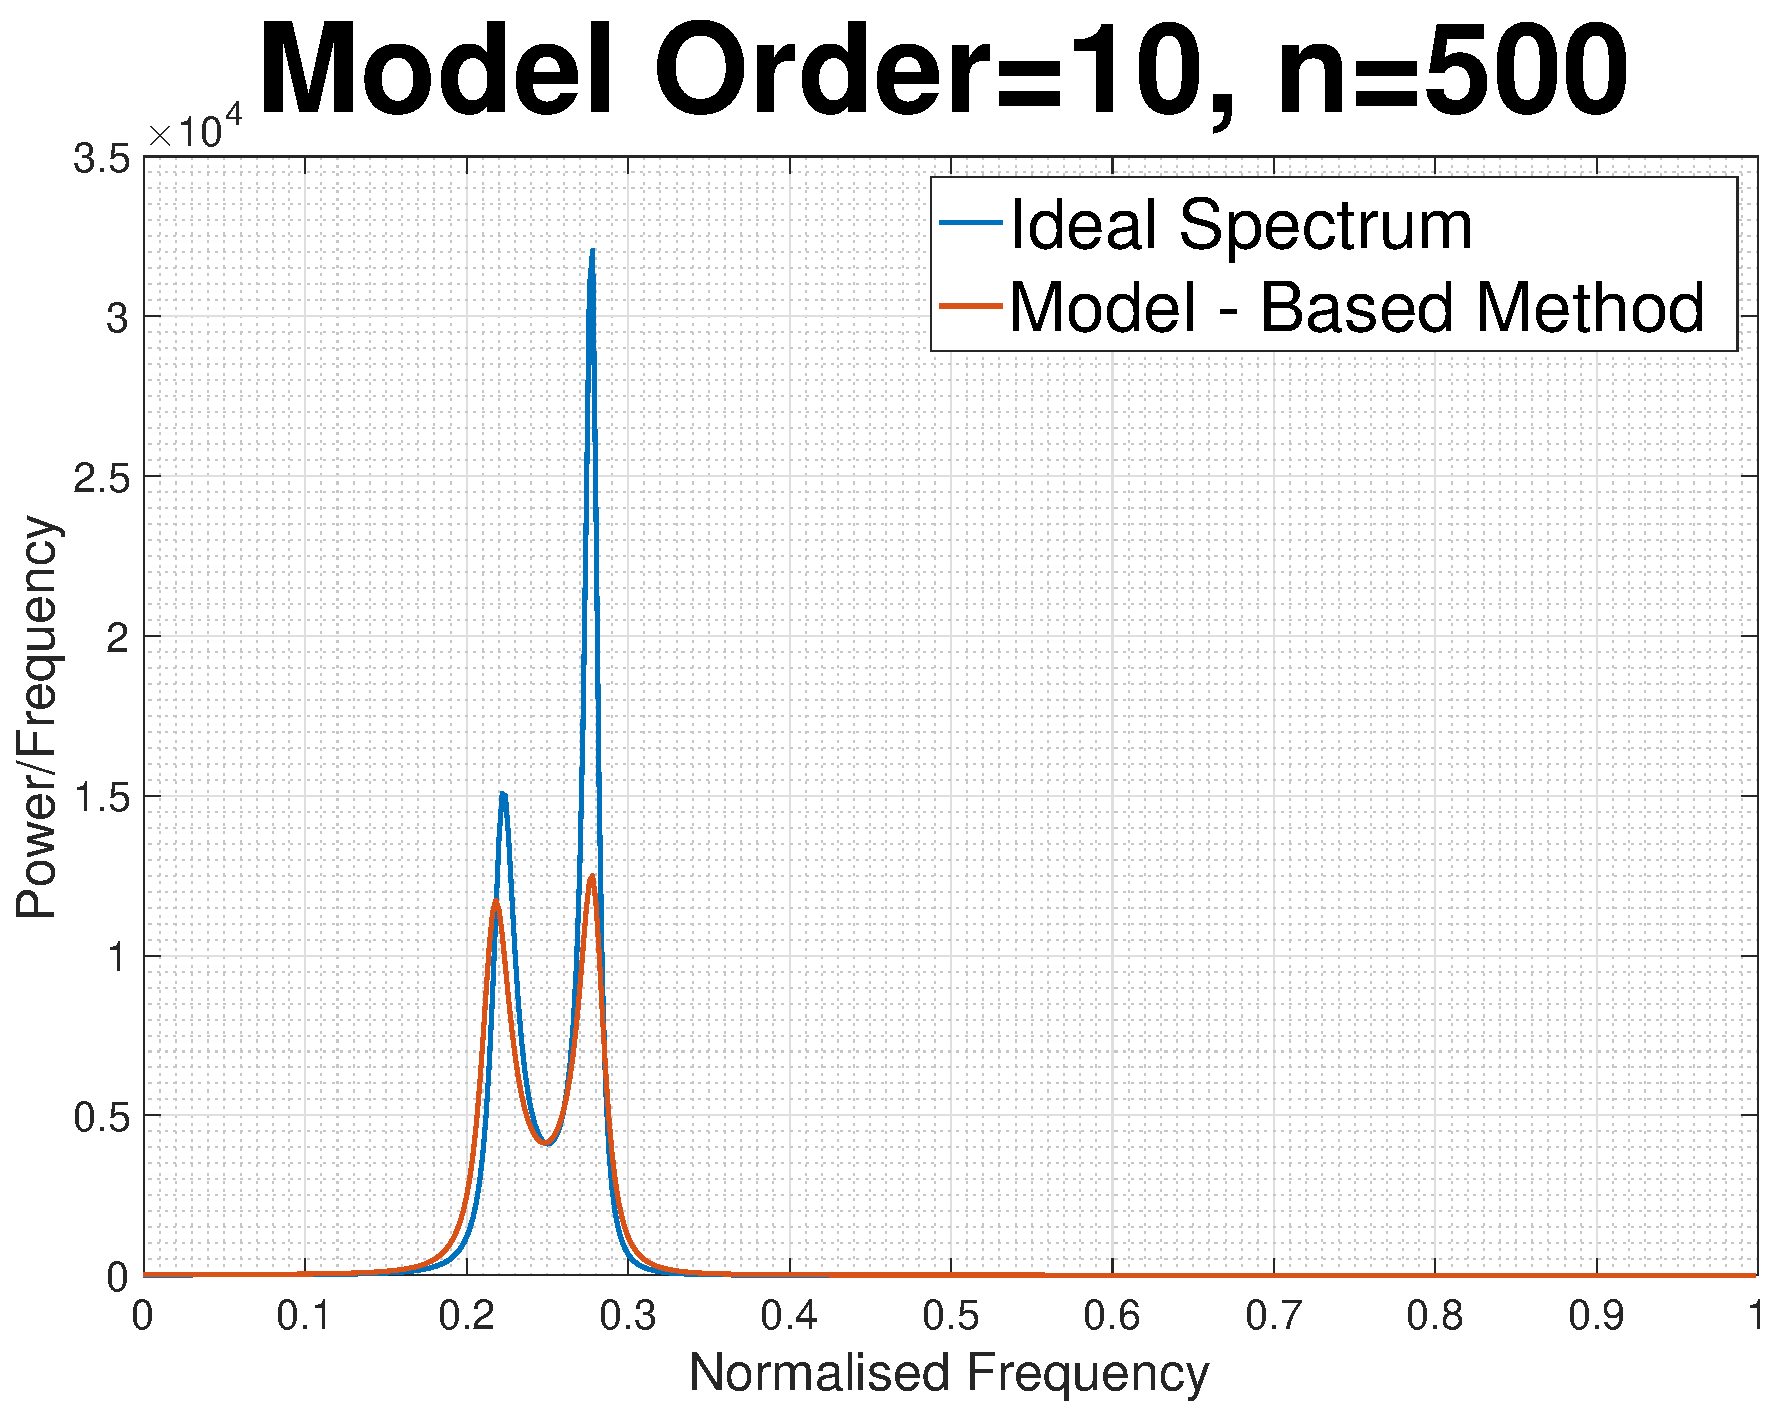
\includegraphics[width=0.24\textwidth]{part2/ar_spectrum_estimate_order_10}
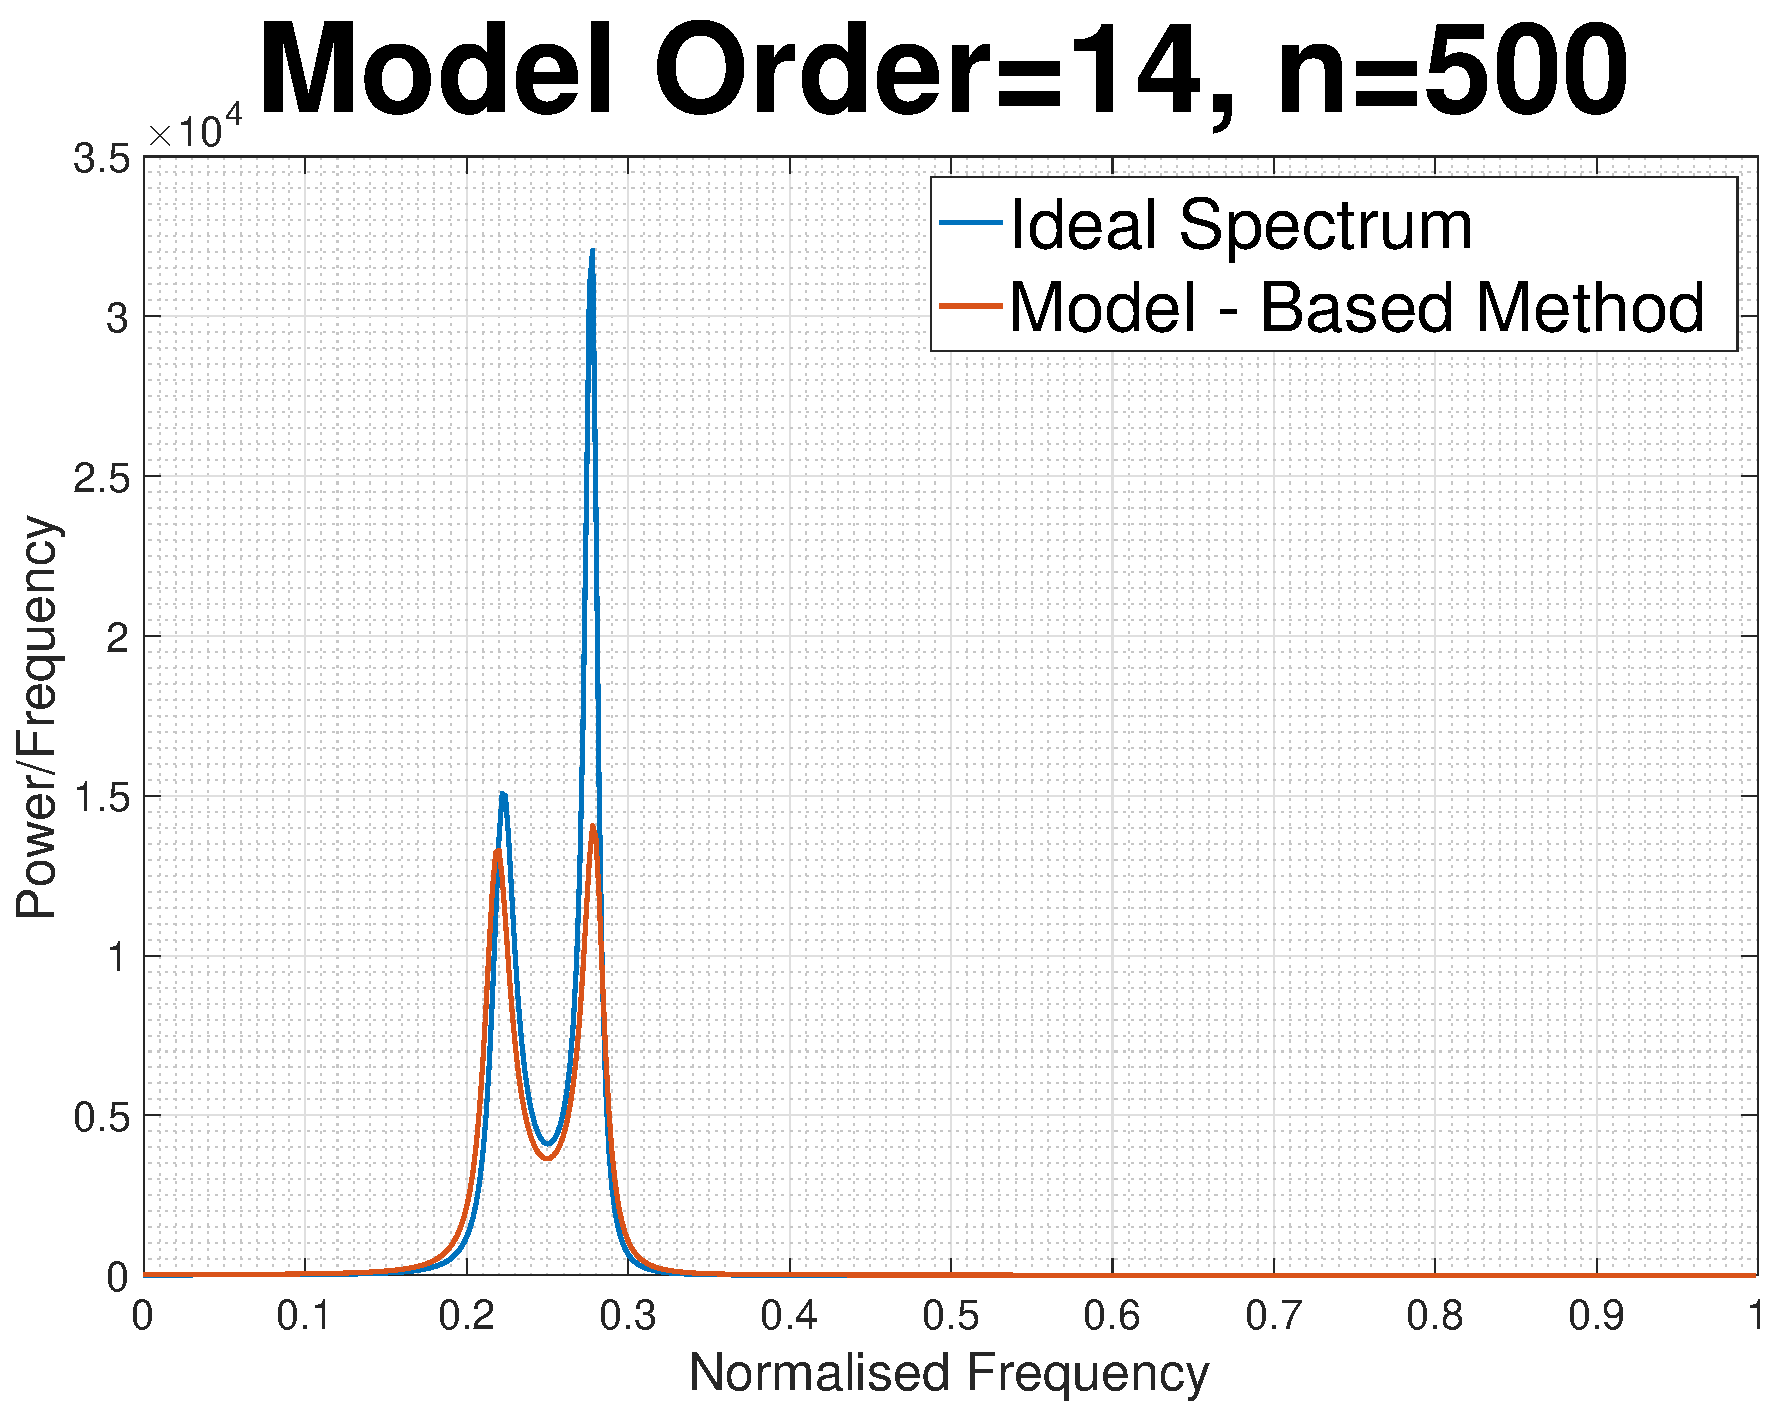
\includegraphics[width=0.24\textwidth]{part2/ar_spectrum_estimate_order_14}
\caption{Power Spectrum Estimates Using All-Pole Autoregressive Model of Orders 4, 8, 10, 14}
\label{fig:AR_1000}
\end{figure}

\noindent{}b. Figure \ref{fig:AR_1000} shows the spectrum obtained when the signal $x(n)$ is modelled as a 4th, 8th, 10th and 14th order AR process. The effects of increasing the model order from $4$ to $8$ is clear. The 4th order process is not able to model the 2 distinct spikes that are present in the ideal spectrum, whereas the 8th order process is. Arbitrarily increasing the model order beyond 8 allows more degrees of freedom since there is greater flexibility to place poles in the spectrum however the resulting spectrum is not more accurate. In fact, increasing the number of poles causes both the peaks to approach the same magnitude; this is obviously not correct. This highlights the fact that the 500 samples used for estimation may not contain enough information about the AR process for effective parameter estimation. \\

\begin{figure}[H]
\centering{}
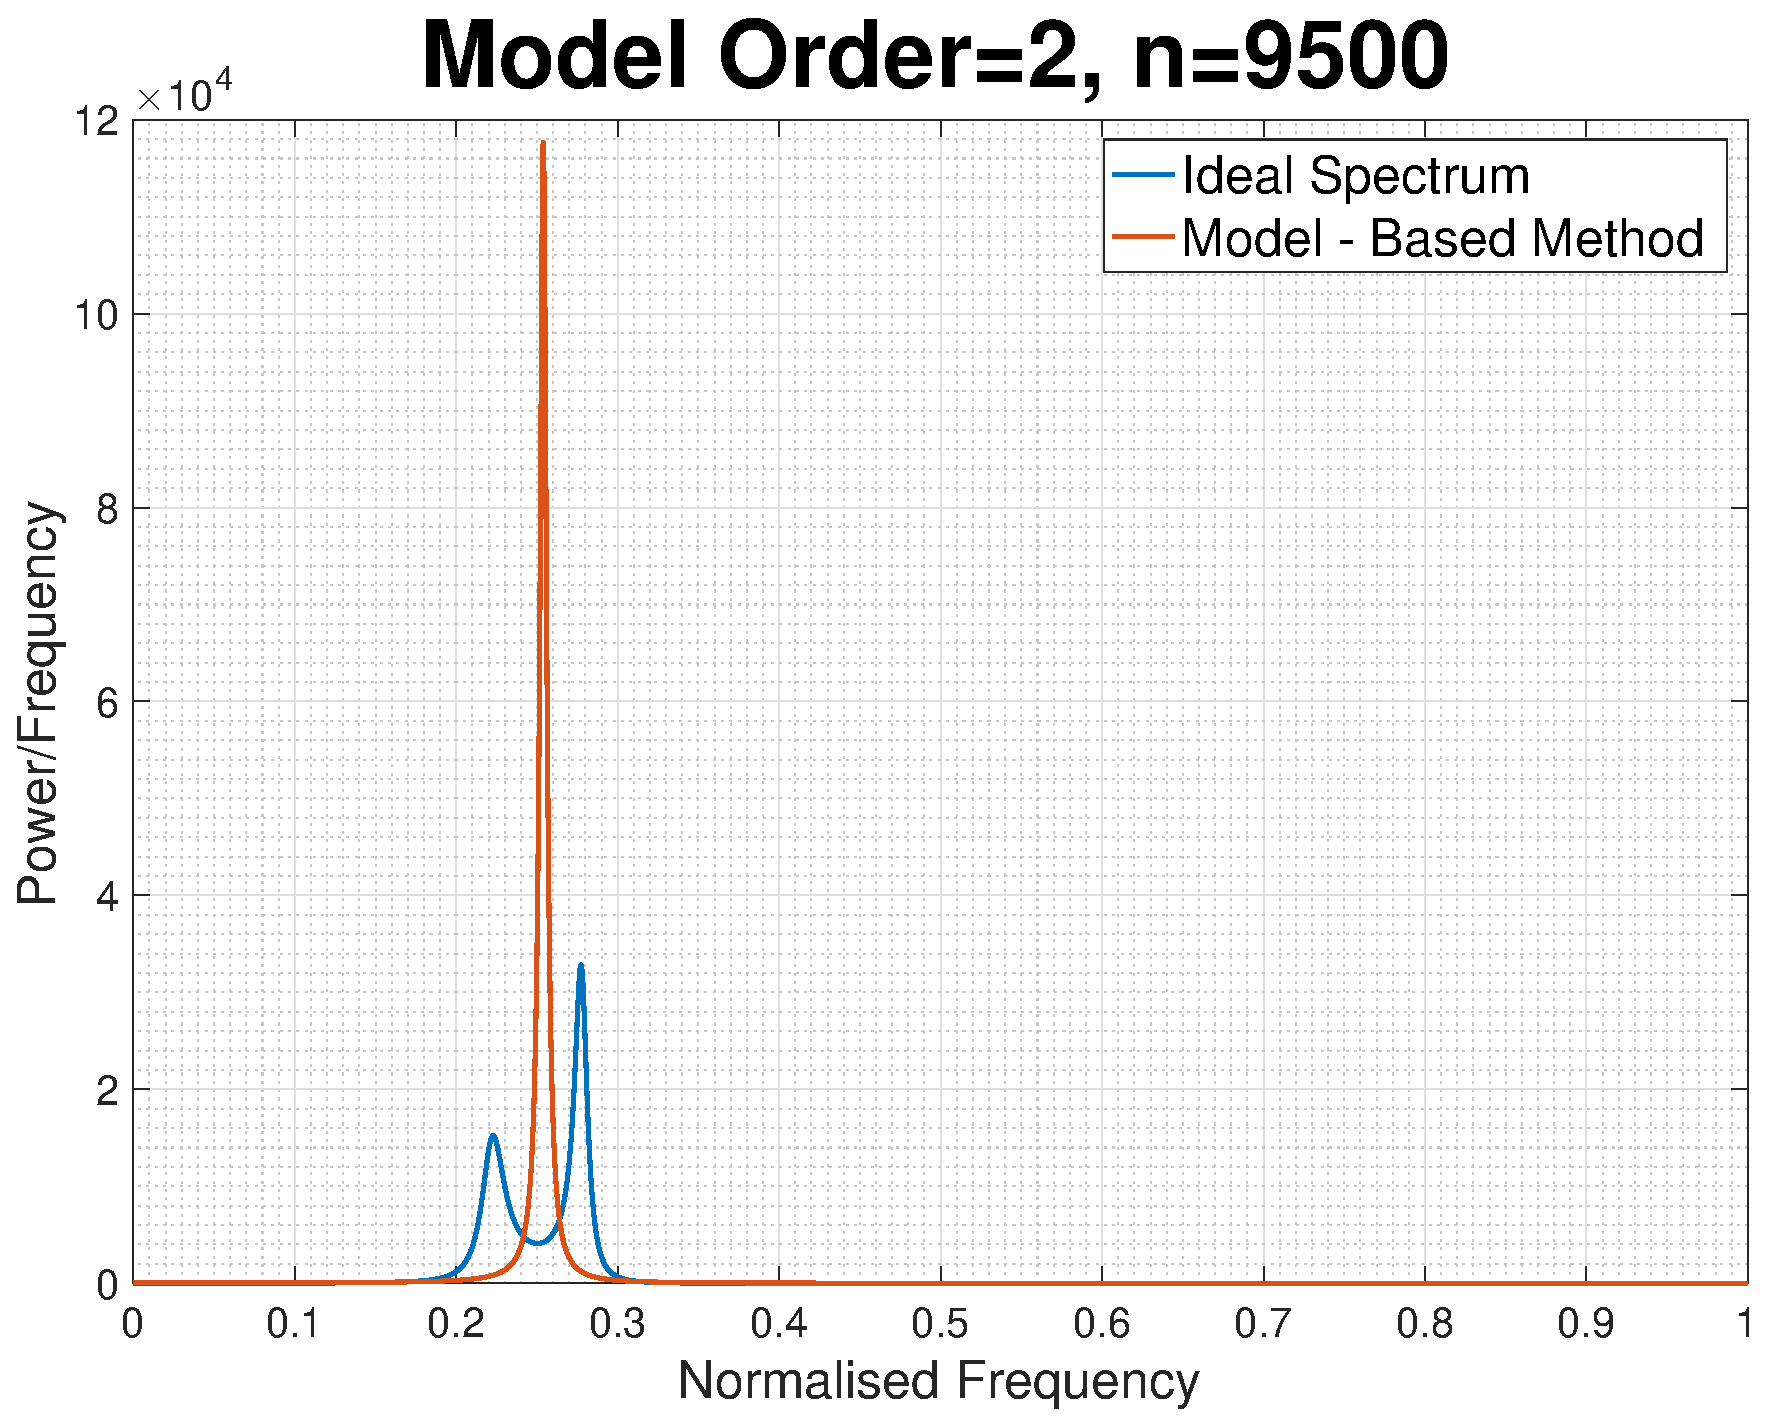
\includegraphics[width=0.32\textwidth]{part2/ar_spectrum_estimate_order_2_9500}
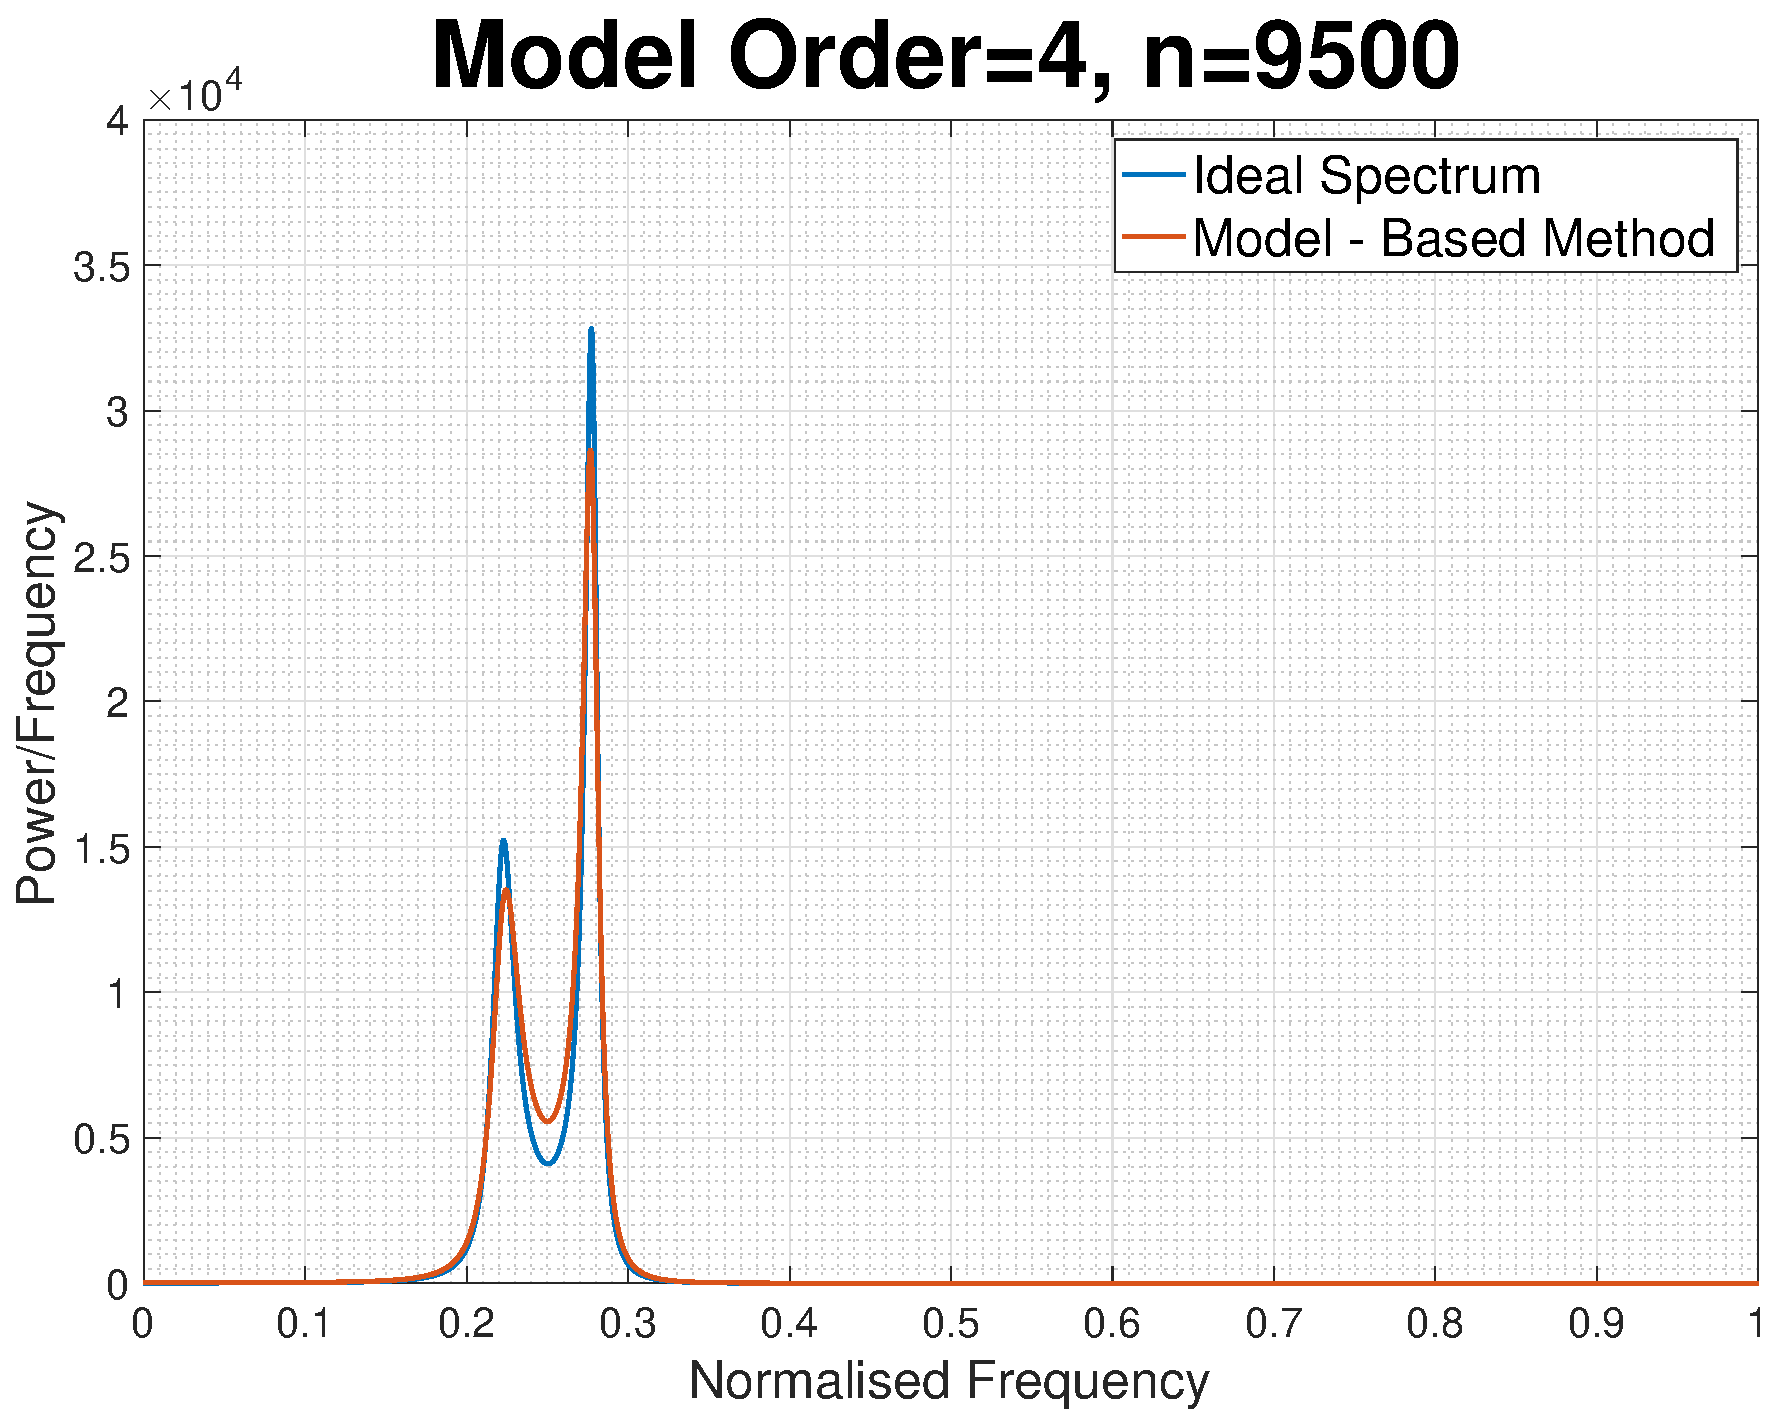
\includegraphics[width=0.32\textwidth]{part2/ar_spectrum_estimate_order_4_9500}
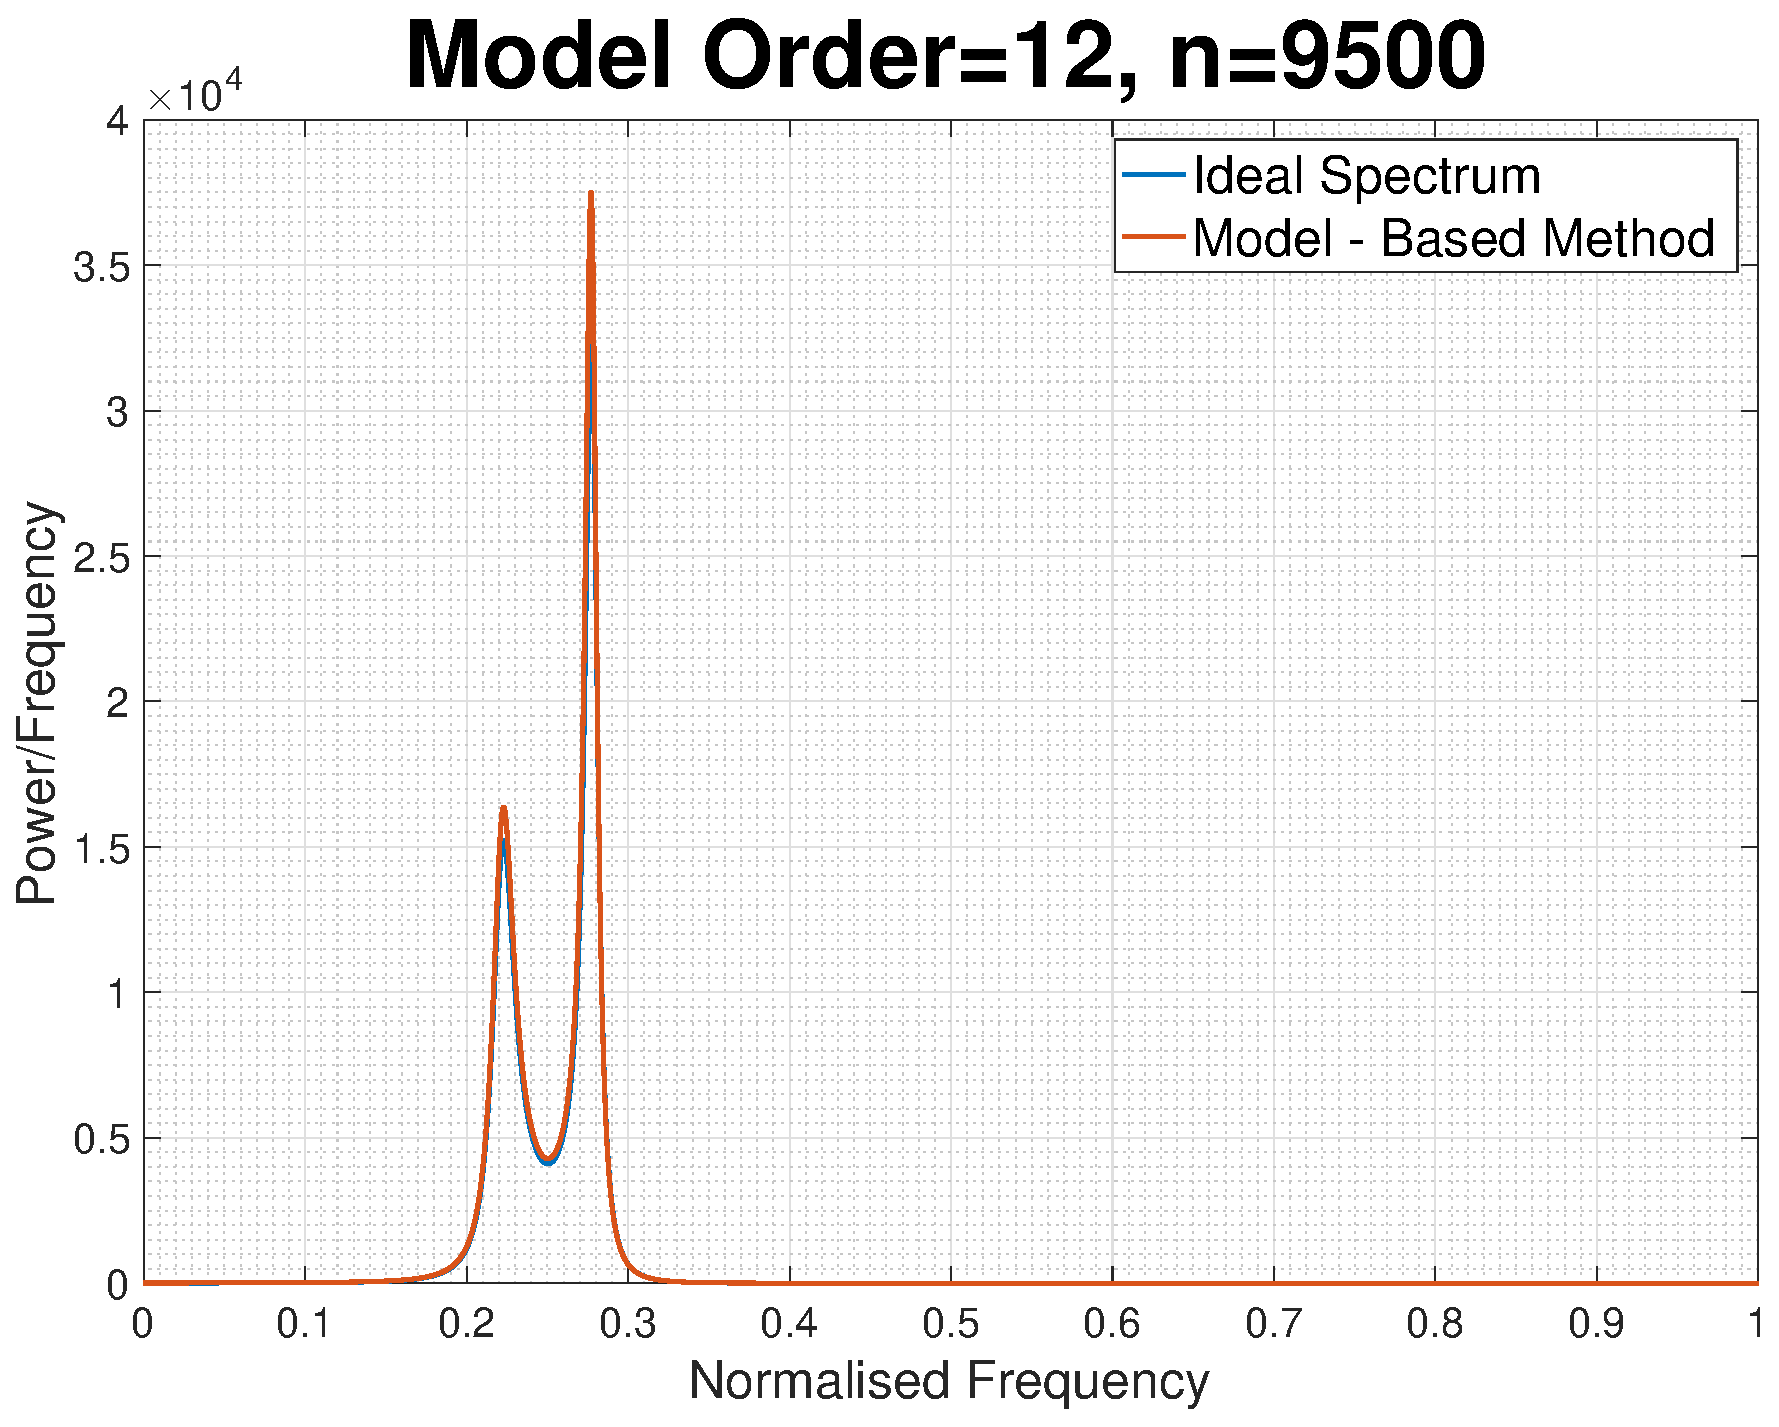
\includegraphics[width=0.32\textwidth]{part2/ar_spectrum_estimate_order_12_9500}
\caption{Effects of Underfitting and Overfitting Autorregressive Models}
\label{fig:AR_10000}
\end{figure}

\noindent{}c. Figure \ref{fig:AR_10000} shows that by increasing the number of samples, we obtain a much more accurate spectrum estimate. The conjecture above about 500 samples not containing enough information about the AR process is correct. Notice that with 10000 samples, a 4th order estimate is able to replicate the two spikes observed in the data. Increasing the model order to 12 shows the problem with overfitting. The peaks of the estimated spectrum have overshot the peak of the ideal spectrum; the power of the signal has been compressed into a small frequency range and thus made it highly periodic. However, by increasing the model order, the estimation error has been reduced. To balance the trade-off between generalization error and estimation error, measures such as the Akaike Information Criterion (AIC) or the Minimum Description Length (MDL) can be used to simulatenously penalize high model orders and estimation errors. 

\begin{figure}[H]
\centering{}
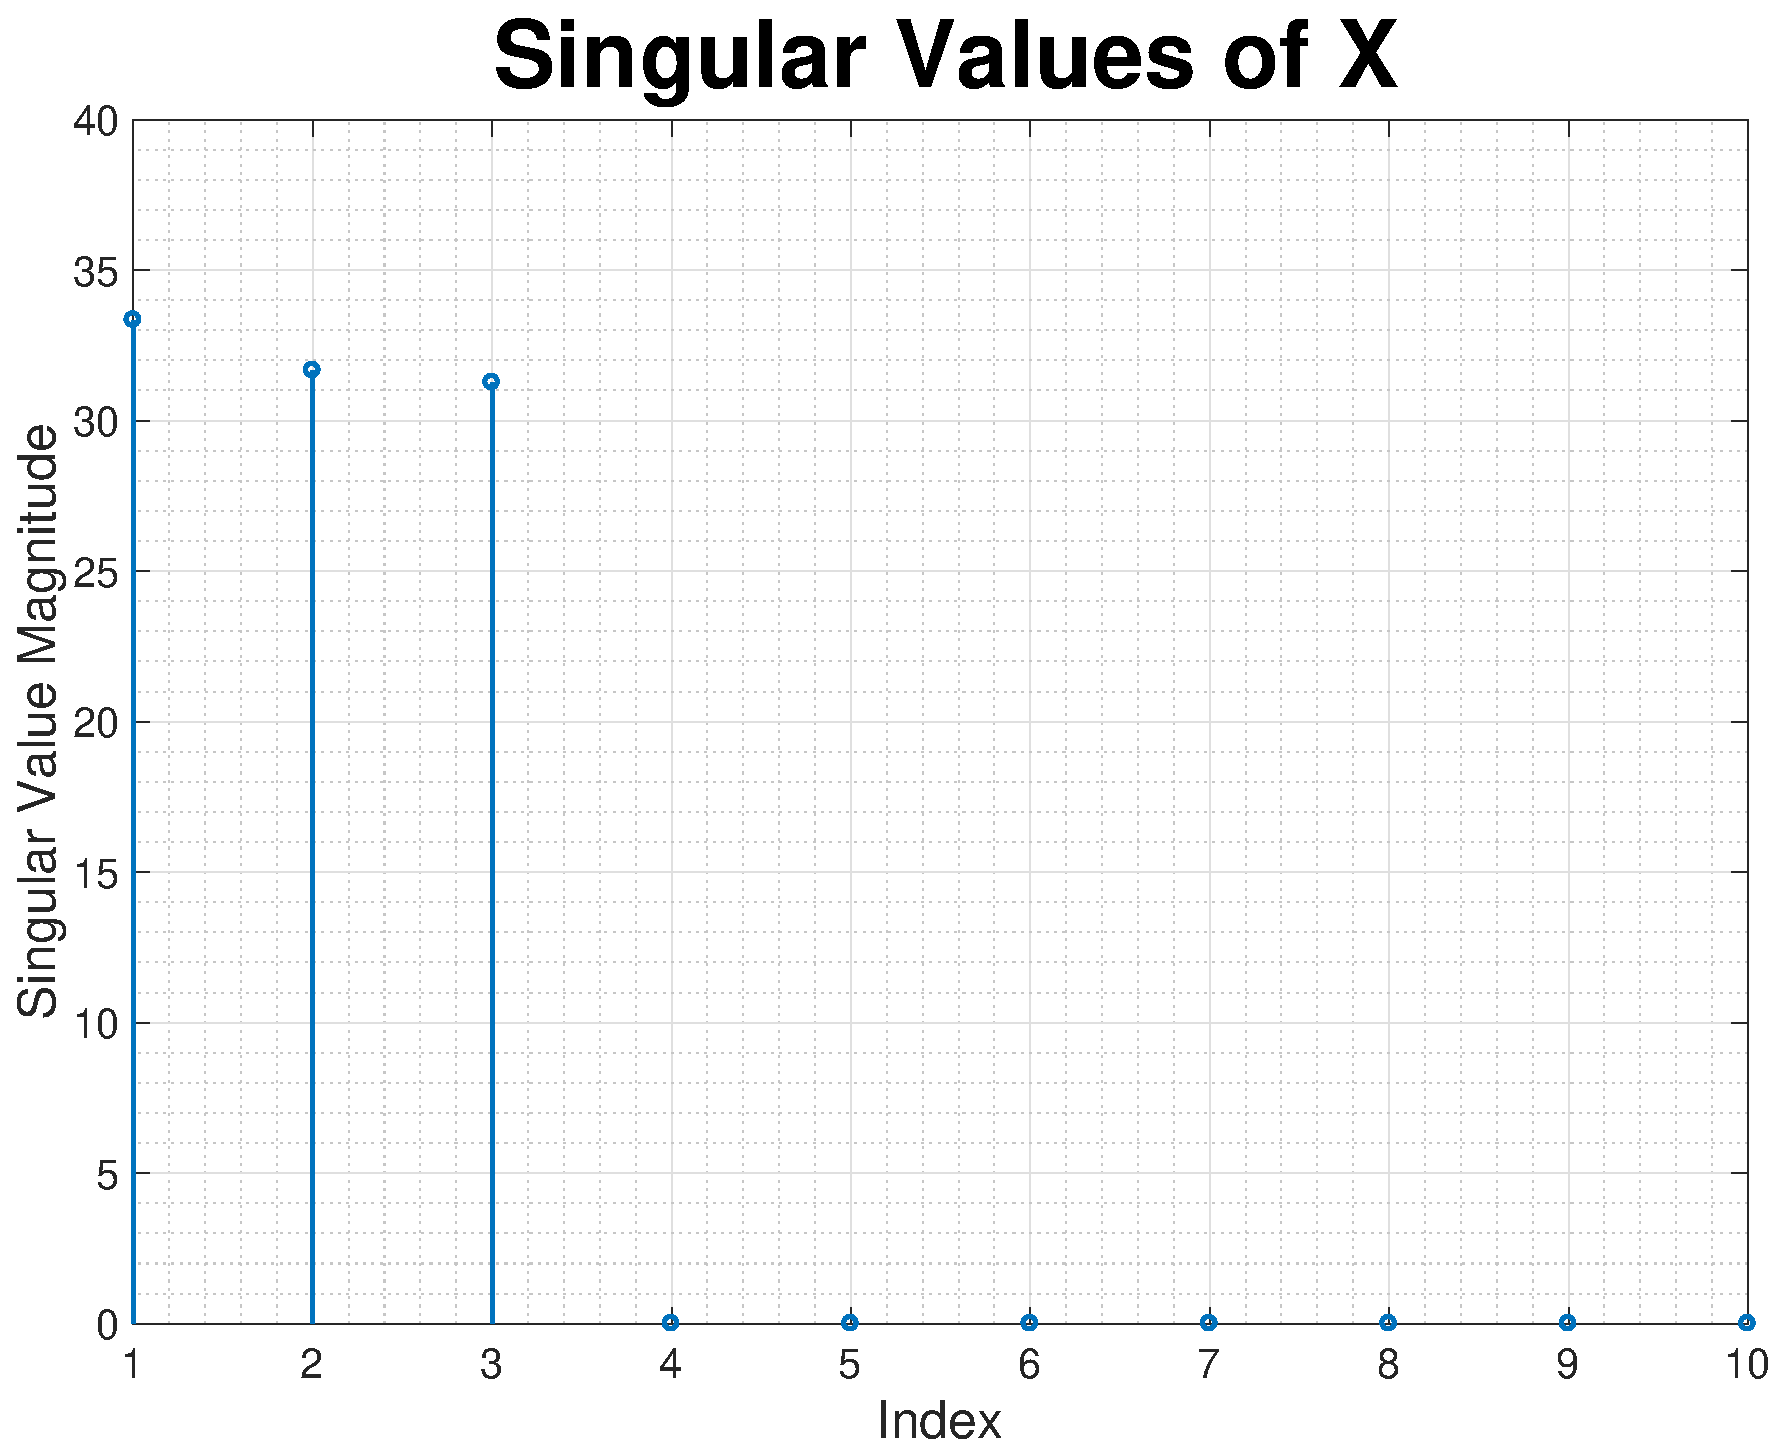
\includegraphics[width=0.32\textwidth]{part2/svd_x}
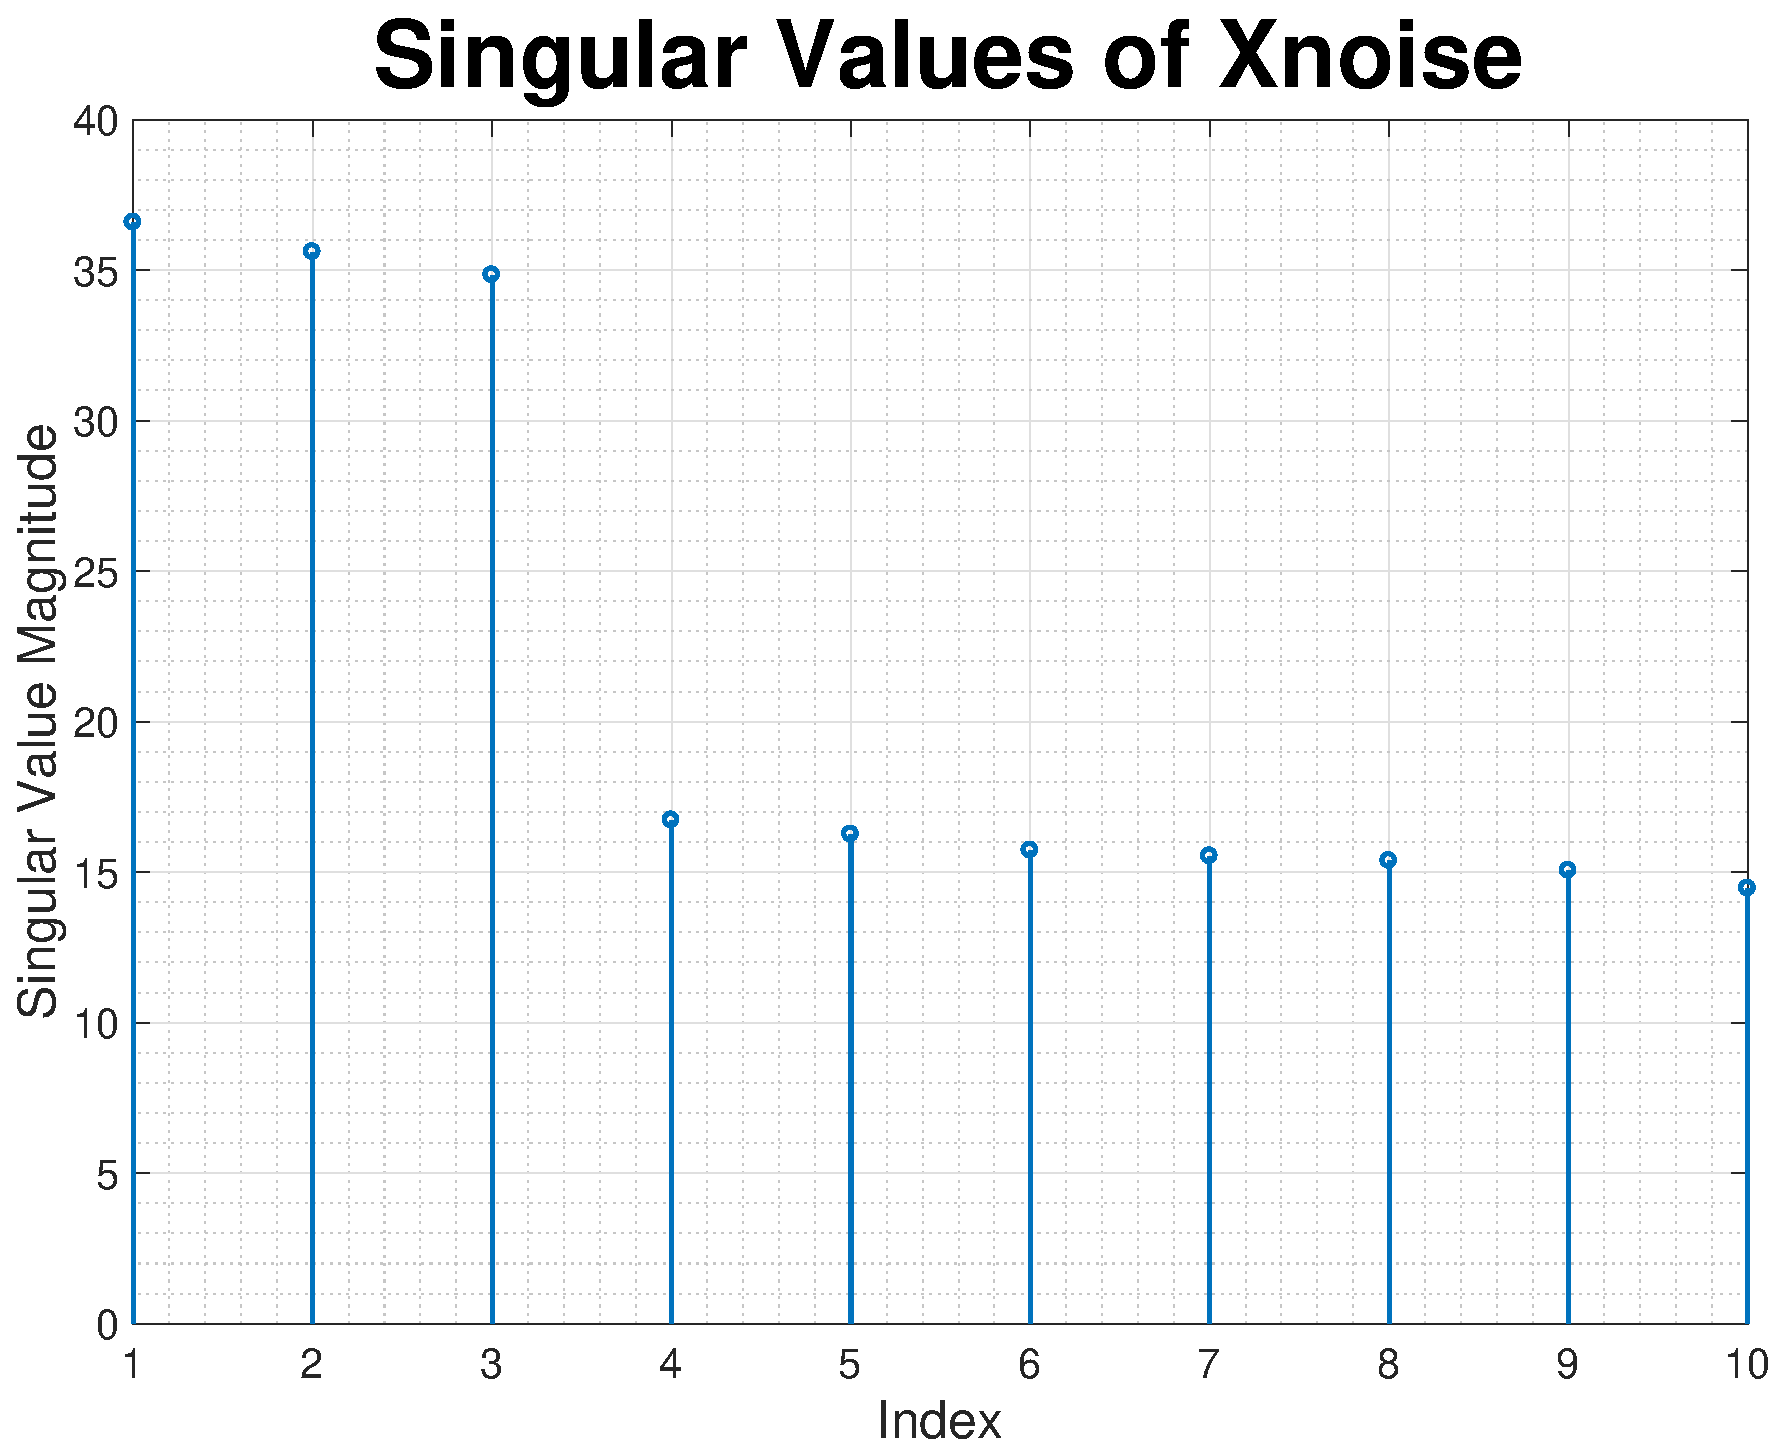
\includegraphics[width=0.32\textwidth]{part2/svd_x_noise}
\caption{Singular Values of Matrices $\textbf{X}$ and $\textbf{X}_{\text{noise}}$}
\end{figure}

\subsection{Real World Signals: Respiratory Sinus Arrhythmia from RR-Intervals}

\noindent{}a. The figure belows shows the standard periodogram obtained for each of the three unique trials of RRI data.

\begin{figure}[H]
\centering{}
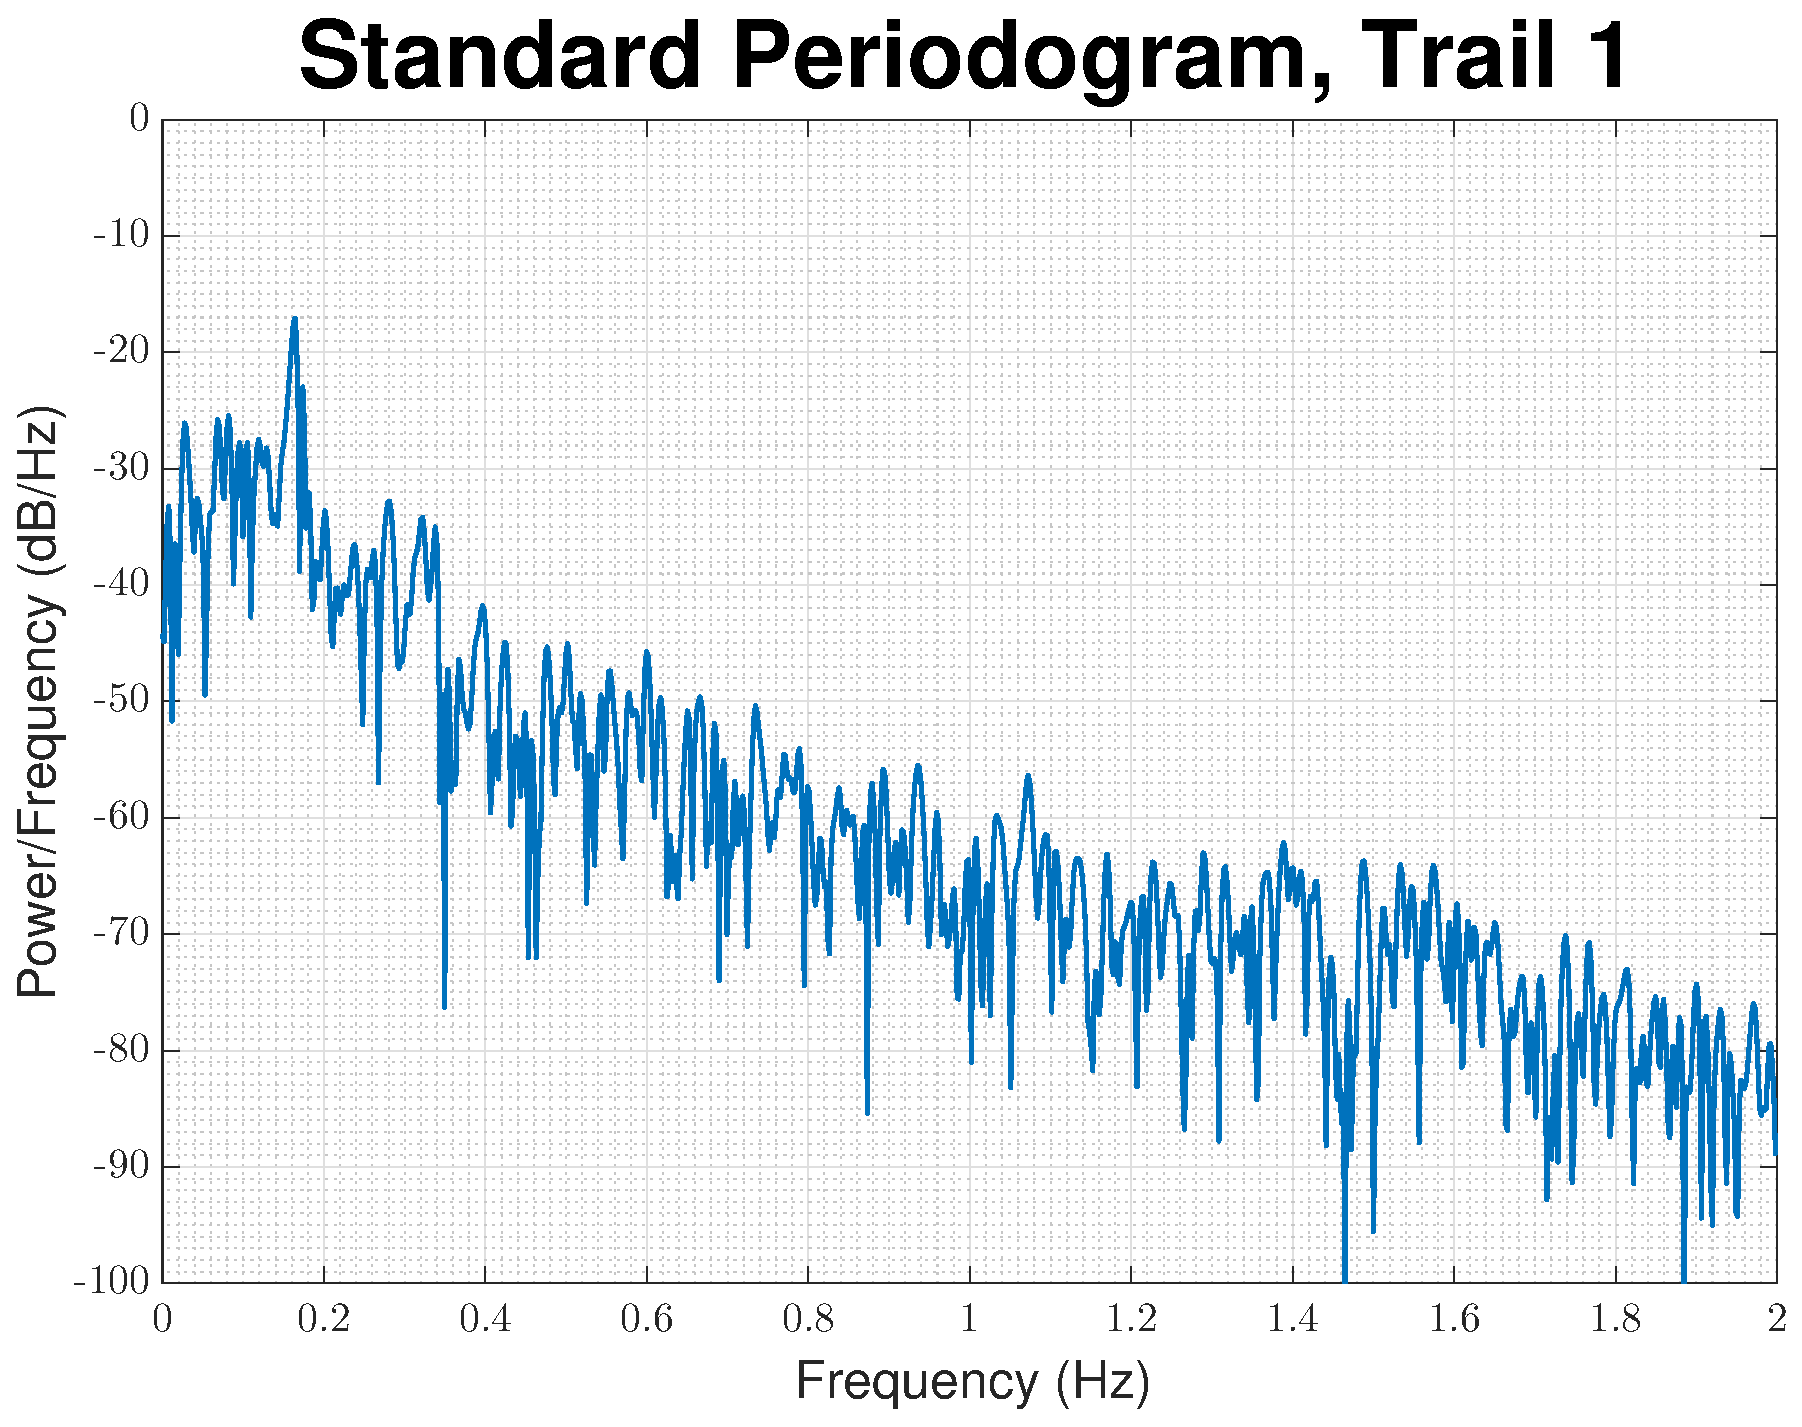
\includegraphics[width=0.32\textwidth]{part2/eeg_trial_1_standard}
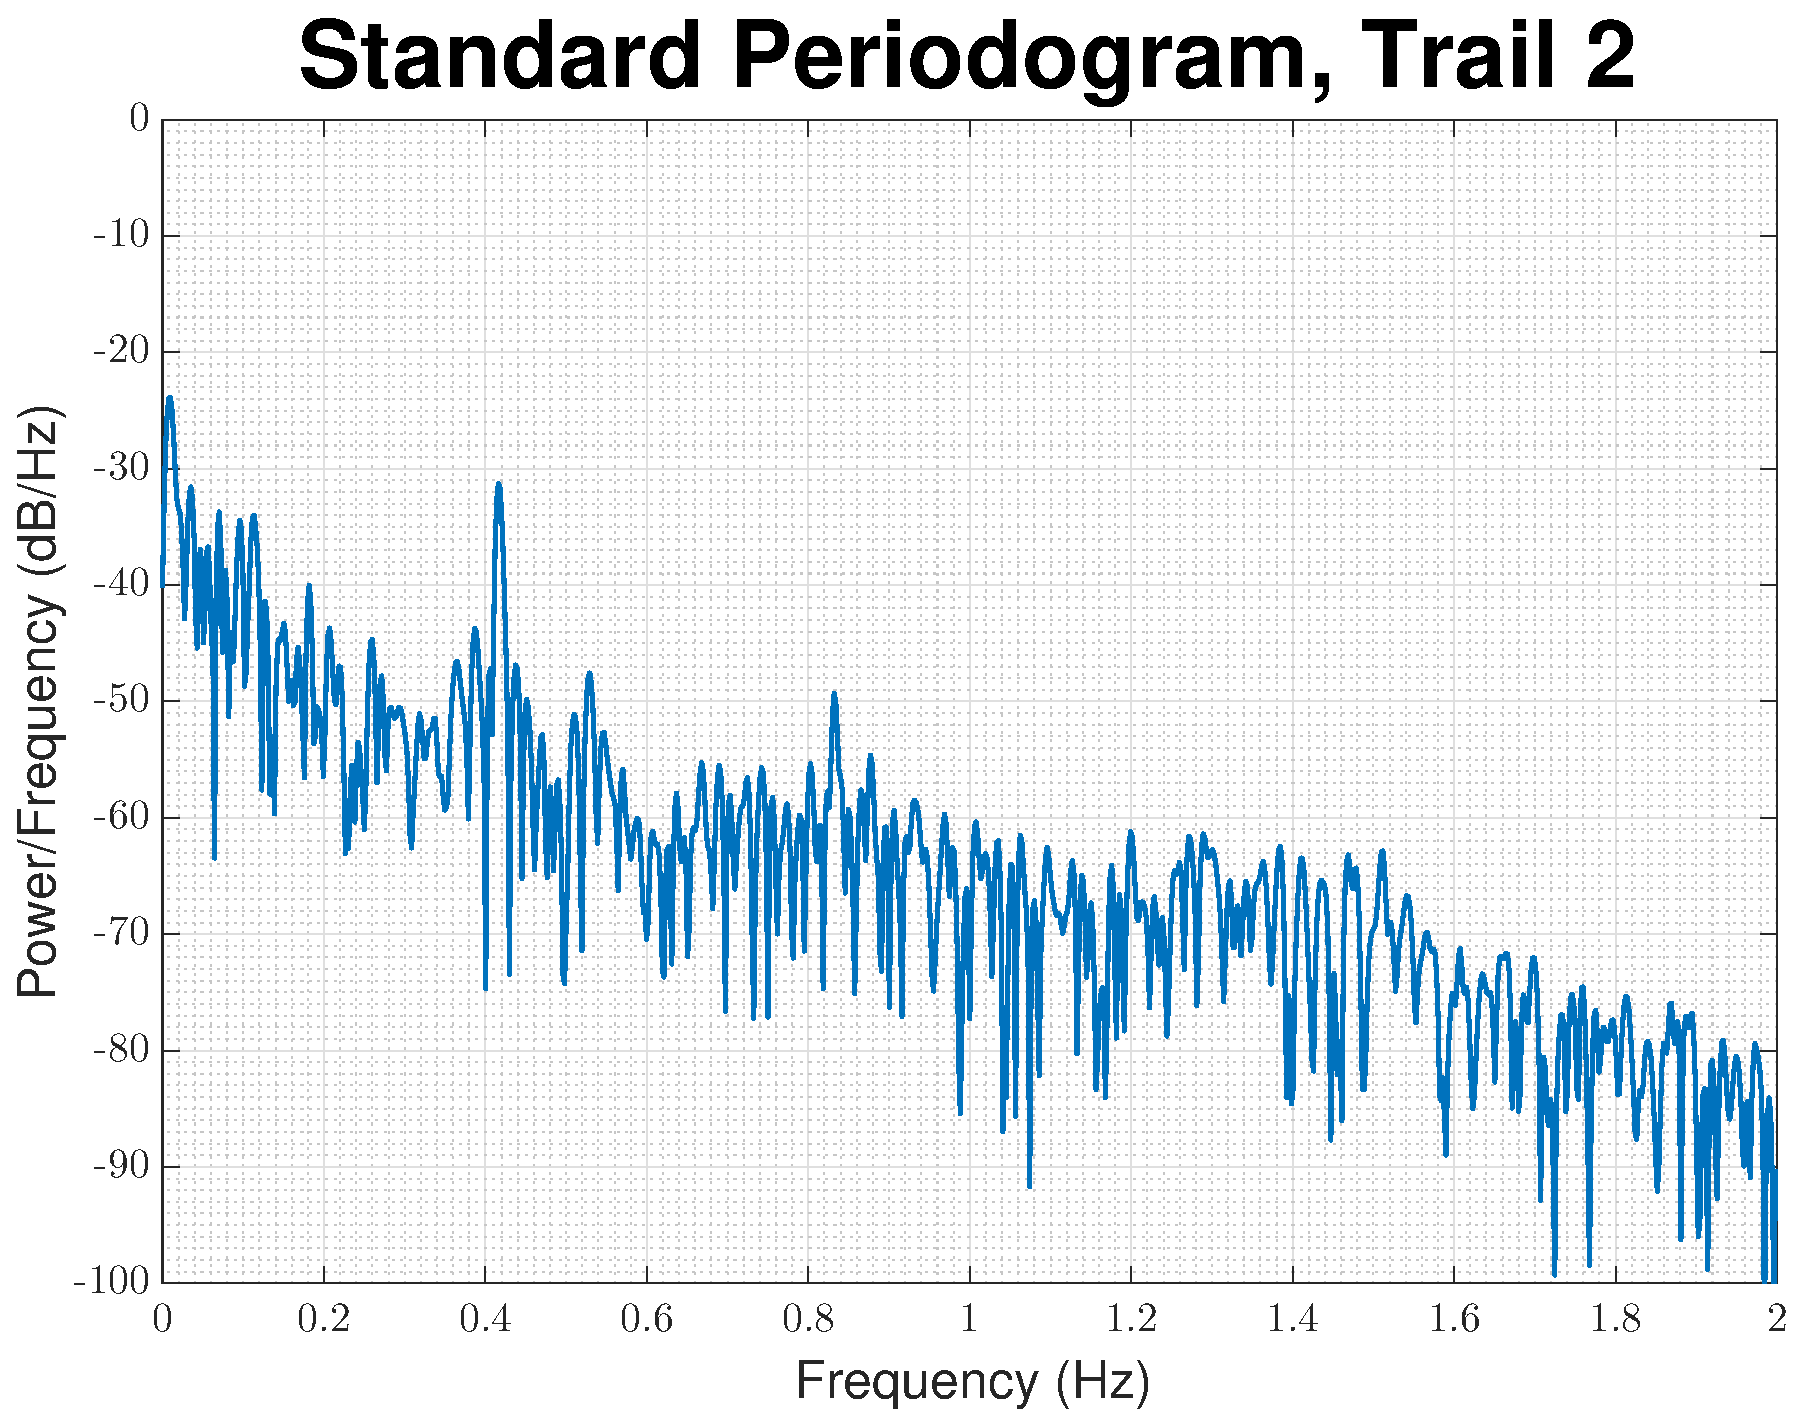
\includegraphics[width=0.32\textwidth]{part2/eeg_trial_2_standard}
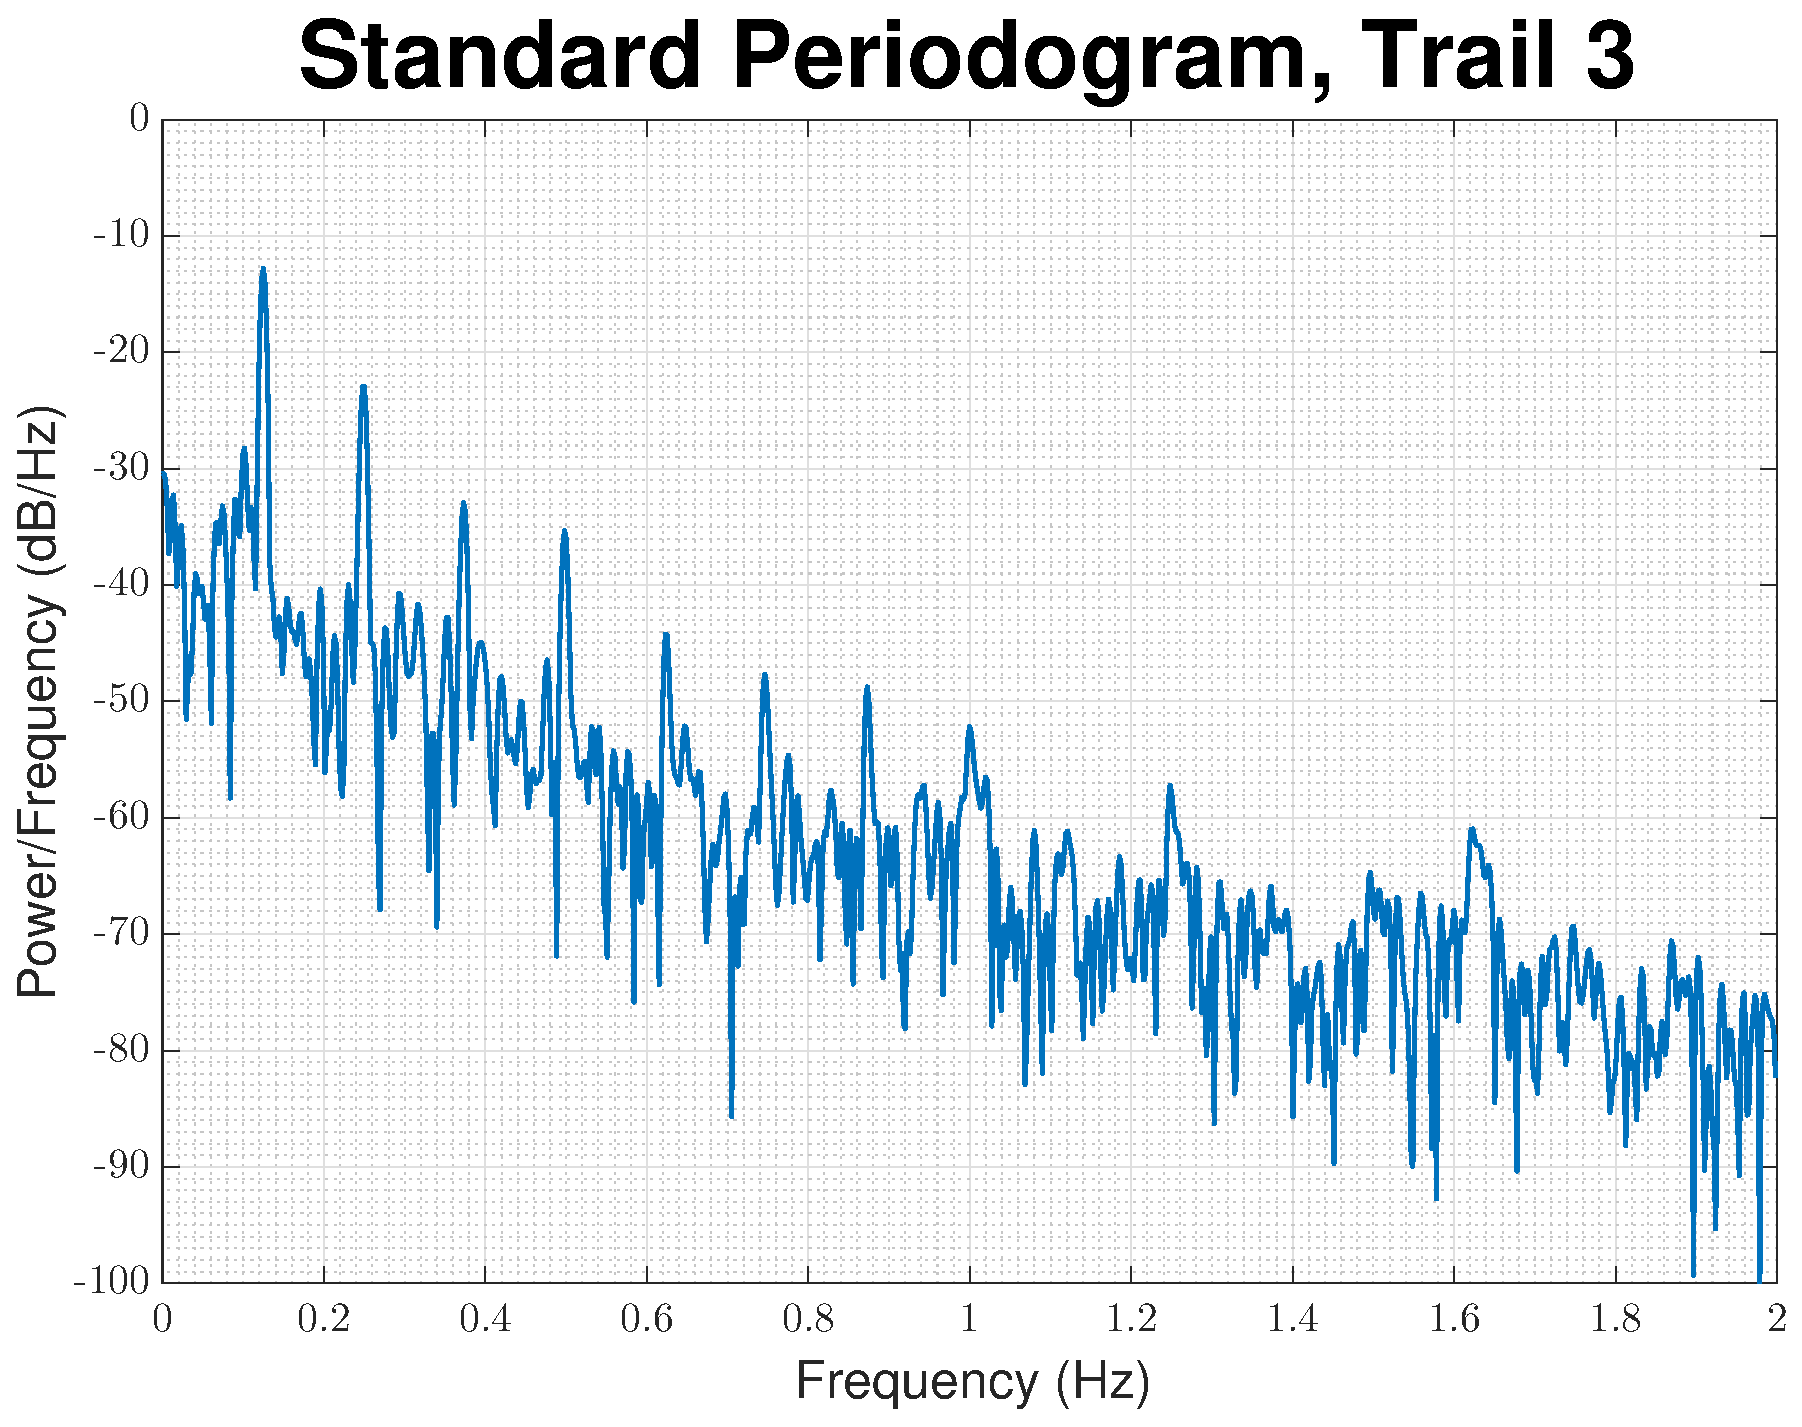
\includegraphics[width=0.32\textwidth]{part2/eeg_trial_3_standard}
\caption{Standard Periodograms of RRI Data obtained from Three Separate Trials}
\end{figure}

\noindent{}The averaged periodogram with different window lengths (50 samples, 150 samples, 200 samples) for three unique trials of RRI data are shown below. Note that the segments used to average the periodogram did not have any overlaps. A hamming window was applied to each segment. The hamming window was developed to minimize the height of the maximum (nearest) side lobe. This minimizes the amount of spectral leakage and produces a spectrum that allows for harmonics of the RSA to be identified in the presence of noise.

\begin{figure}[H]
\centering{}
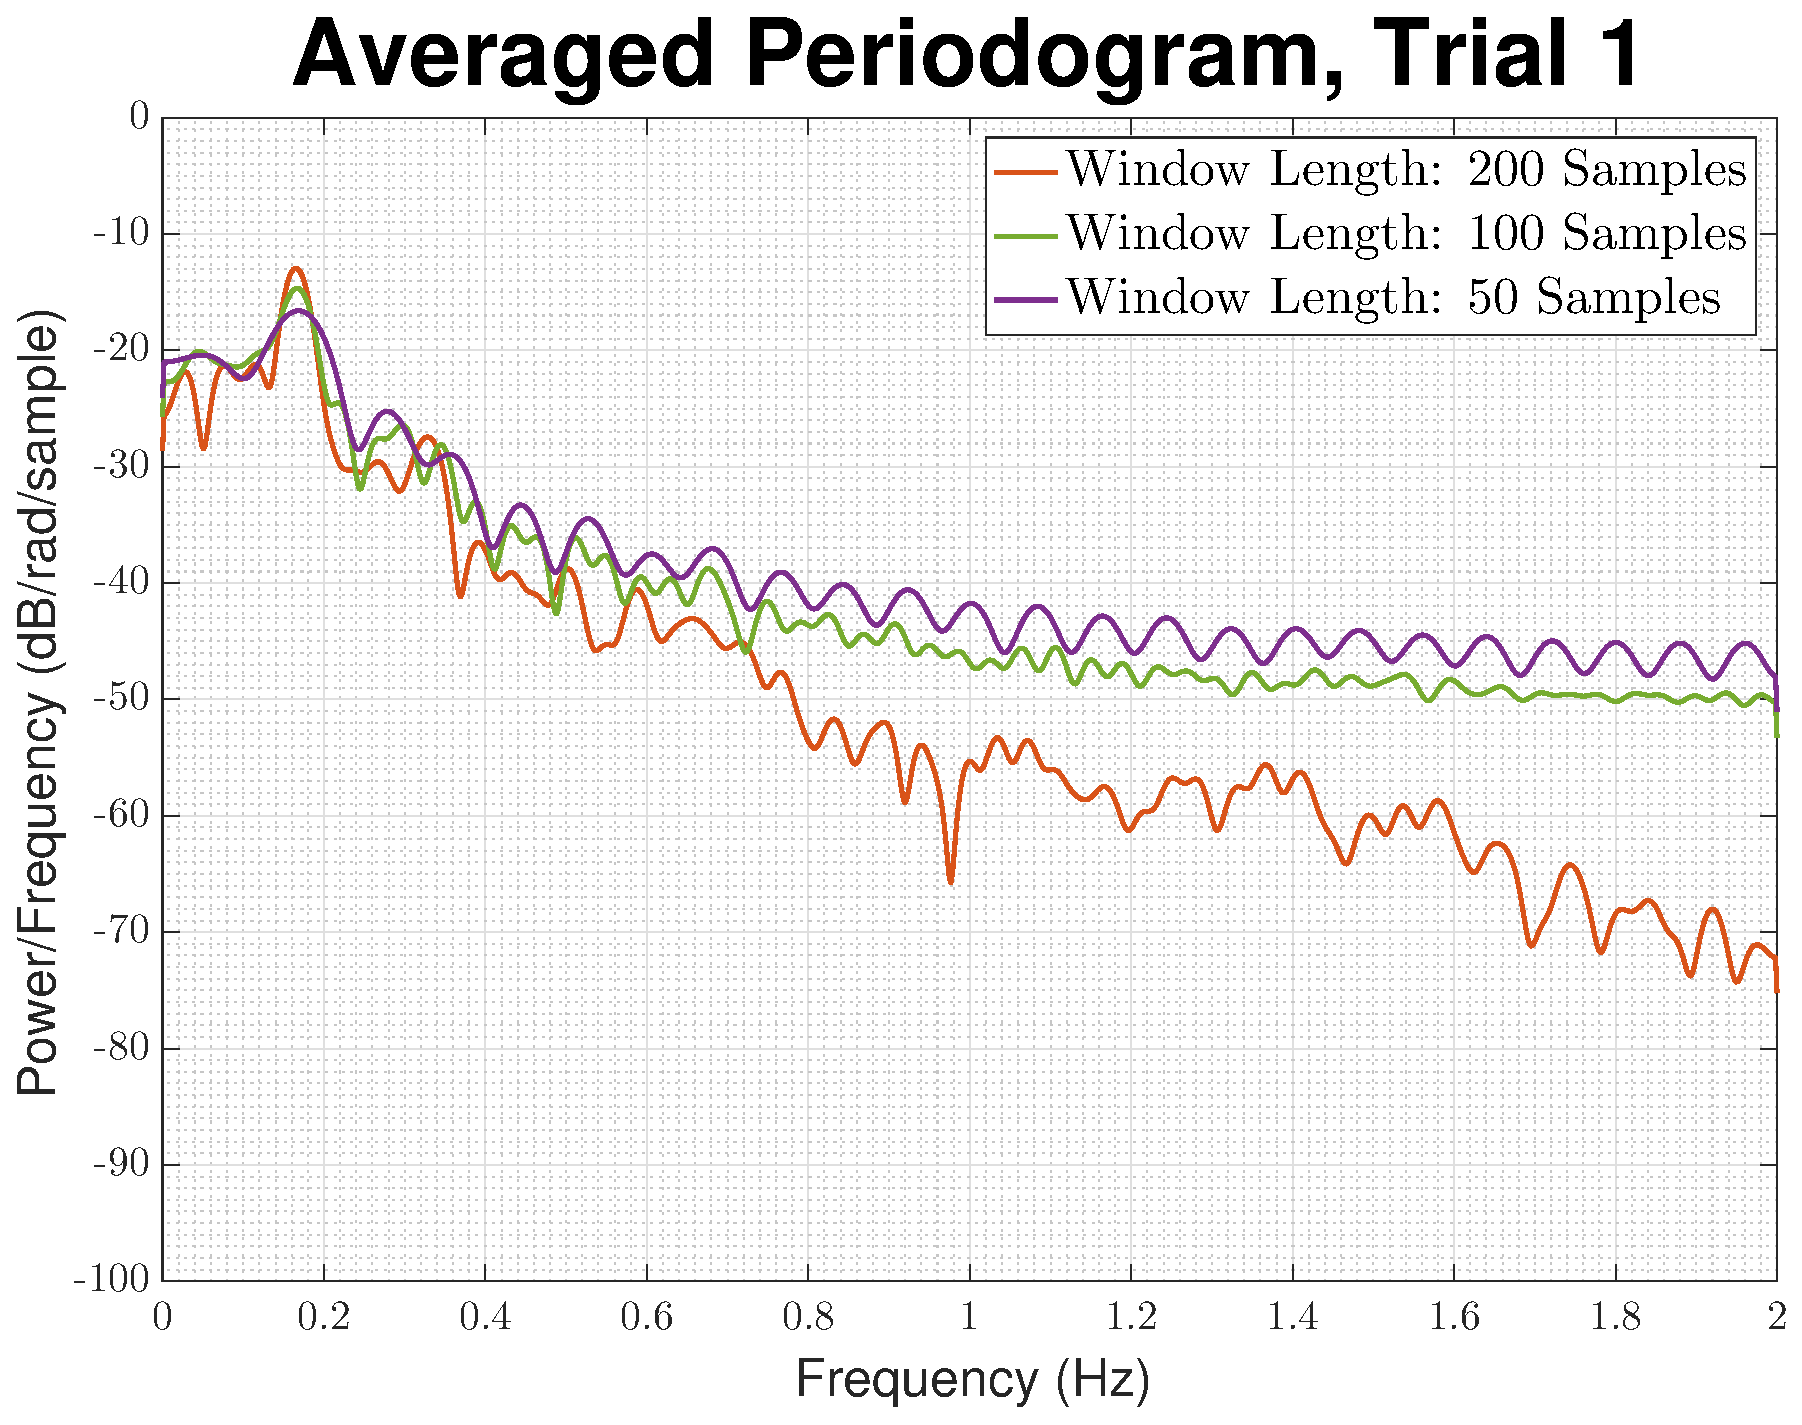
\includegraphics[width=0.32\textwidth]{part2/eeg_trial_1_averaged}
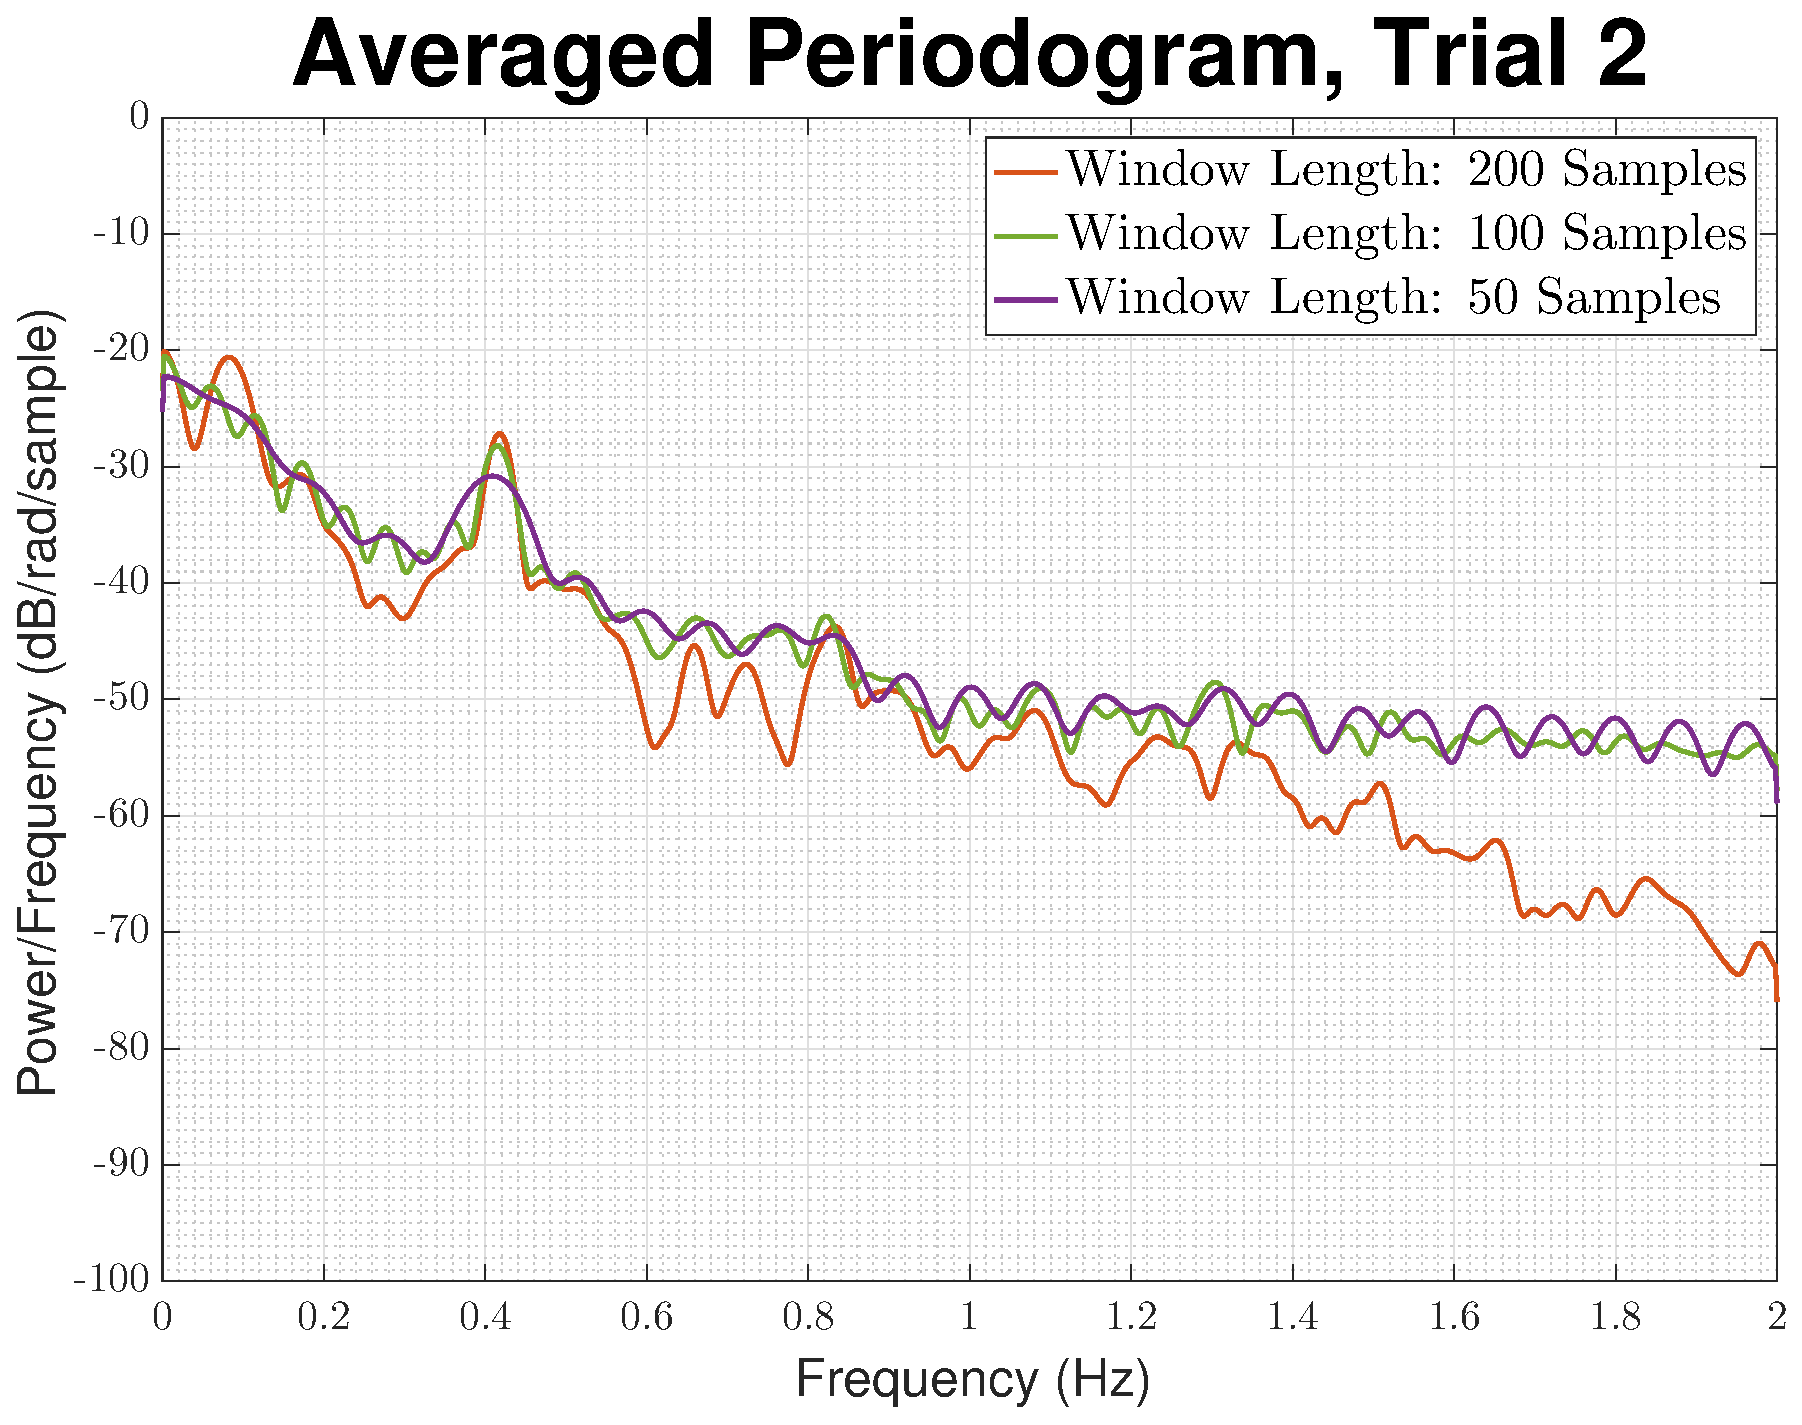
\includegraphics[width=0.32\textwidth]{part2/eeg_trial_2_averaged}
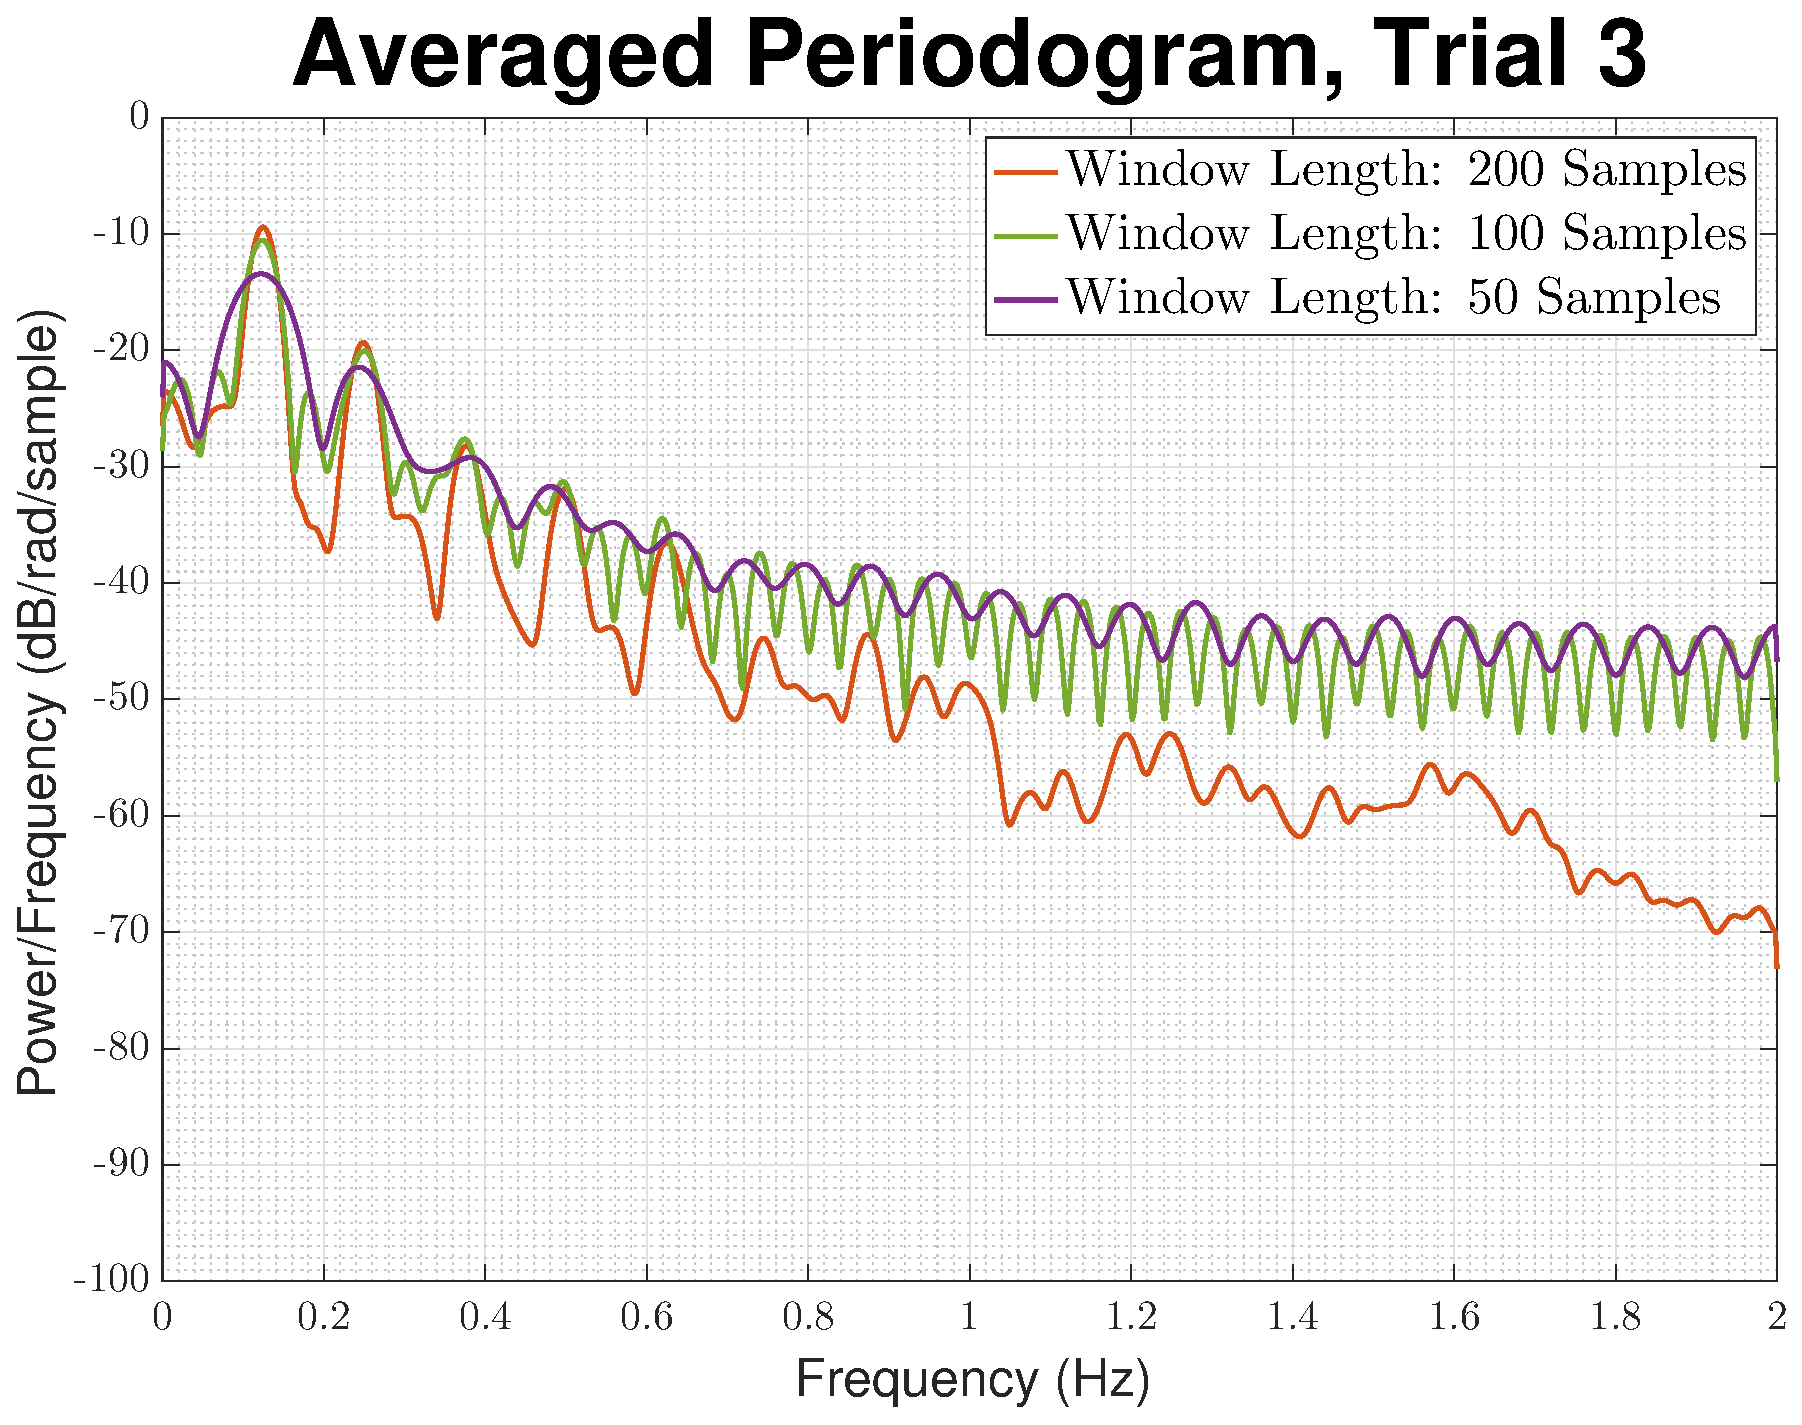
\includegraphics[width=0.32\textwidth]{part2/eeg_trial_3_averaged}
\caption{Averaged Periodograms, with Different Window Lengths, of RRI Data obtained from Three Separate Trials}
\end{figure}

\noindent{}b. Note that the three trials were conducted in such a way that:
\begin{enumerate}
\item Trial 1: Unconstrained Breathing, Typical Ventilation Rate 20-45 Breaths Per Minute (BPM)
\item Trial 2: Fast Breathing, Ventilation Rate 50 BPM
\item Trial 3: Slow Breathing, Ventilation Rate 15 BPM
\end{enumerate}

\noindent{}With this in mind, we study the standard periodograms and note that the first harmonics of the RSA for each trial are:
\begin{enumerate}
\item Trial 1: Peak at 0.1641 Hz, which implies a breathing rate of $2*60*0.1641 = 19.69 \approx 20$ BPM
\item Trial 2: Peak at 0.416 Hz, which implies a breathing rate of $2*60*0.416 = 49.92 \approx 50$ BPM
\item Trial 3: Peak at 0.125 Hz, which implies a breathing rate of $2*60*0.125 = 15$ BPM
\end{enumerate}

\noindent{}We study the averaged periodograms and find that they produce smoother estimates because increasing the number of samples for which we average the periodogram means that the variance of the estimate decreases. Averaging over 200 samples, the 2nd harmonic in Trial 1 at $f=0.332$ Hz is clear. This harmonic cannot be distinguished in the standard periodogram. In fact, when averaged over 50 and 100 samples, the peak of the 2nd harmonic does not occur at $f=0.332$ Hz; the peaks actually occur at $f=0.2773$ Hz and $f=0.2949$ Hz for the 50 samples and 100 samples periodograms respectively. This means that, in an attempt to remove noise, by averaging over smaller segments, we have lost the resolution and the ability to correctly identify the 2nd harmonic. Similarly, for other trials, harmonics are much more evident in the averaged periodogram with a small shift introduced when averaged over 50 and 100 samples.\\

\noindent{}c. The figure below shows the results obtained when the RRI data is modeled as an AR process. For Trial 1, it is impossible to fit an AR model that models any harmonic beyond the fundamental. This is because of the fact that in the original signal, the only significant periodic component occurs at $f=0.1641$ Hz. As such, increasing the model order amplifies the peak at $f=0.1641$ Hz instead of introducing more peak. In contrast, the averaged periodogram, when averaged over 200 sample segments, is able to model the harmonics well. In addition, notice that beyond order 10, an artifact starts to occur at 1.5 Hz. This is not present in the averaged periodogram.

\begin{figure}[H]
\centering{}
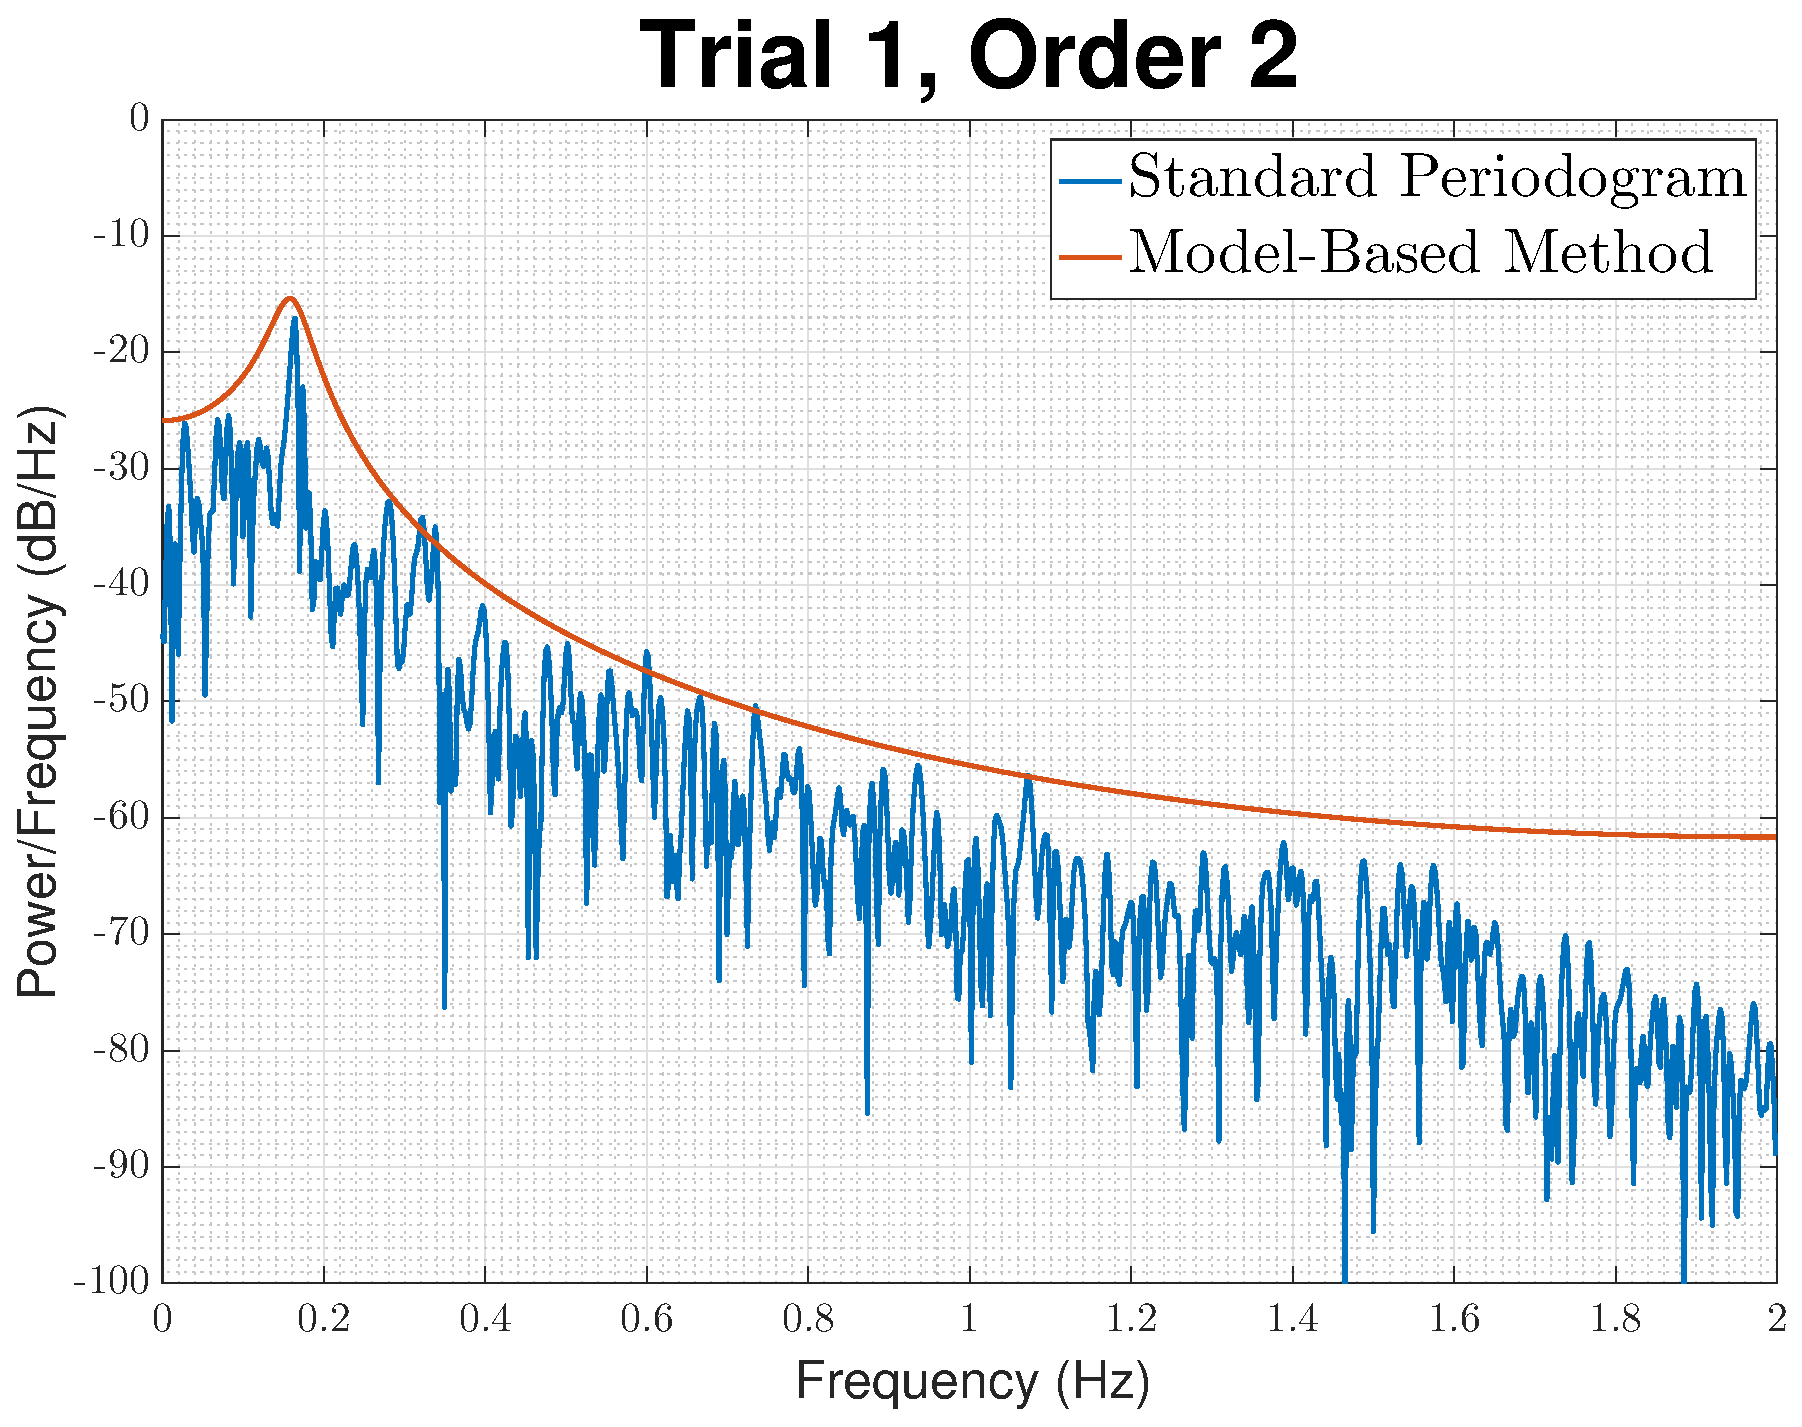
\includegraphics[width=0.32\textwidth]{part2/ar_spectrum_eeg_trial_1_order_2}
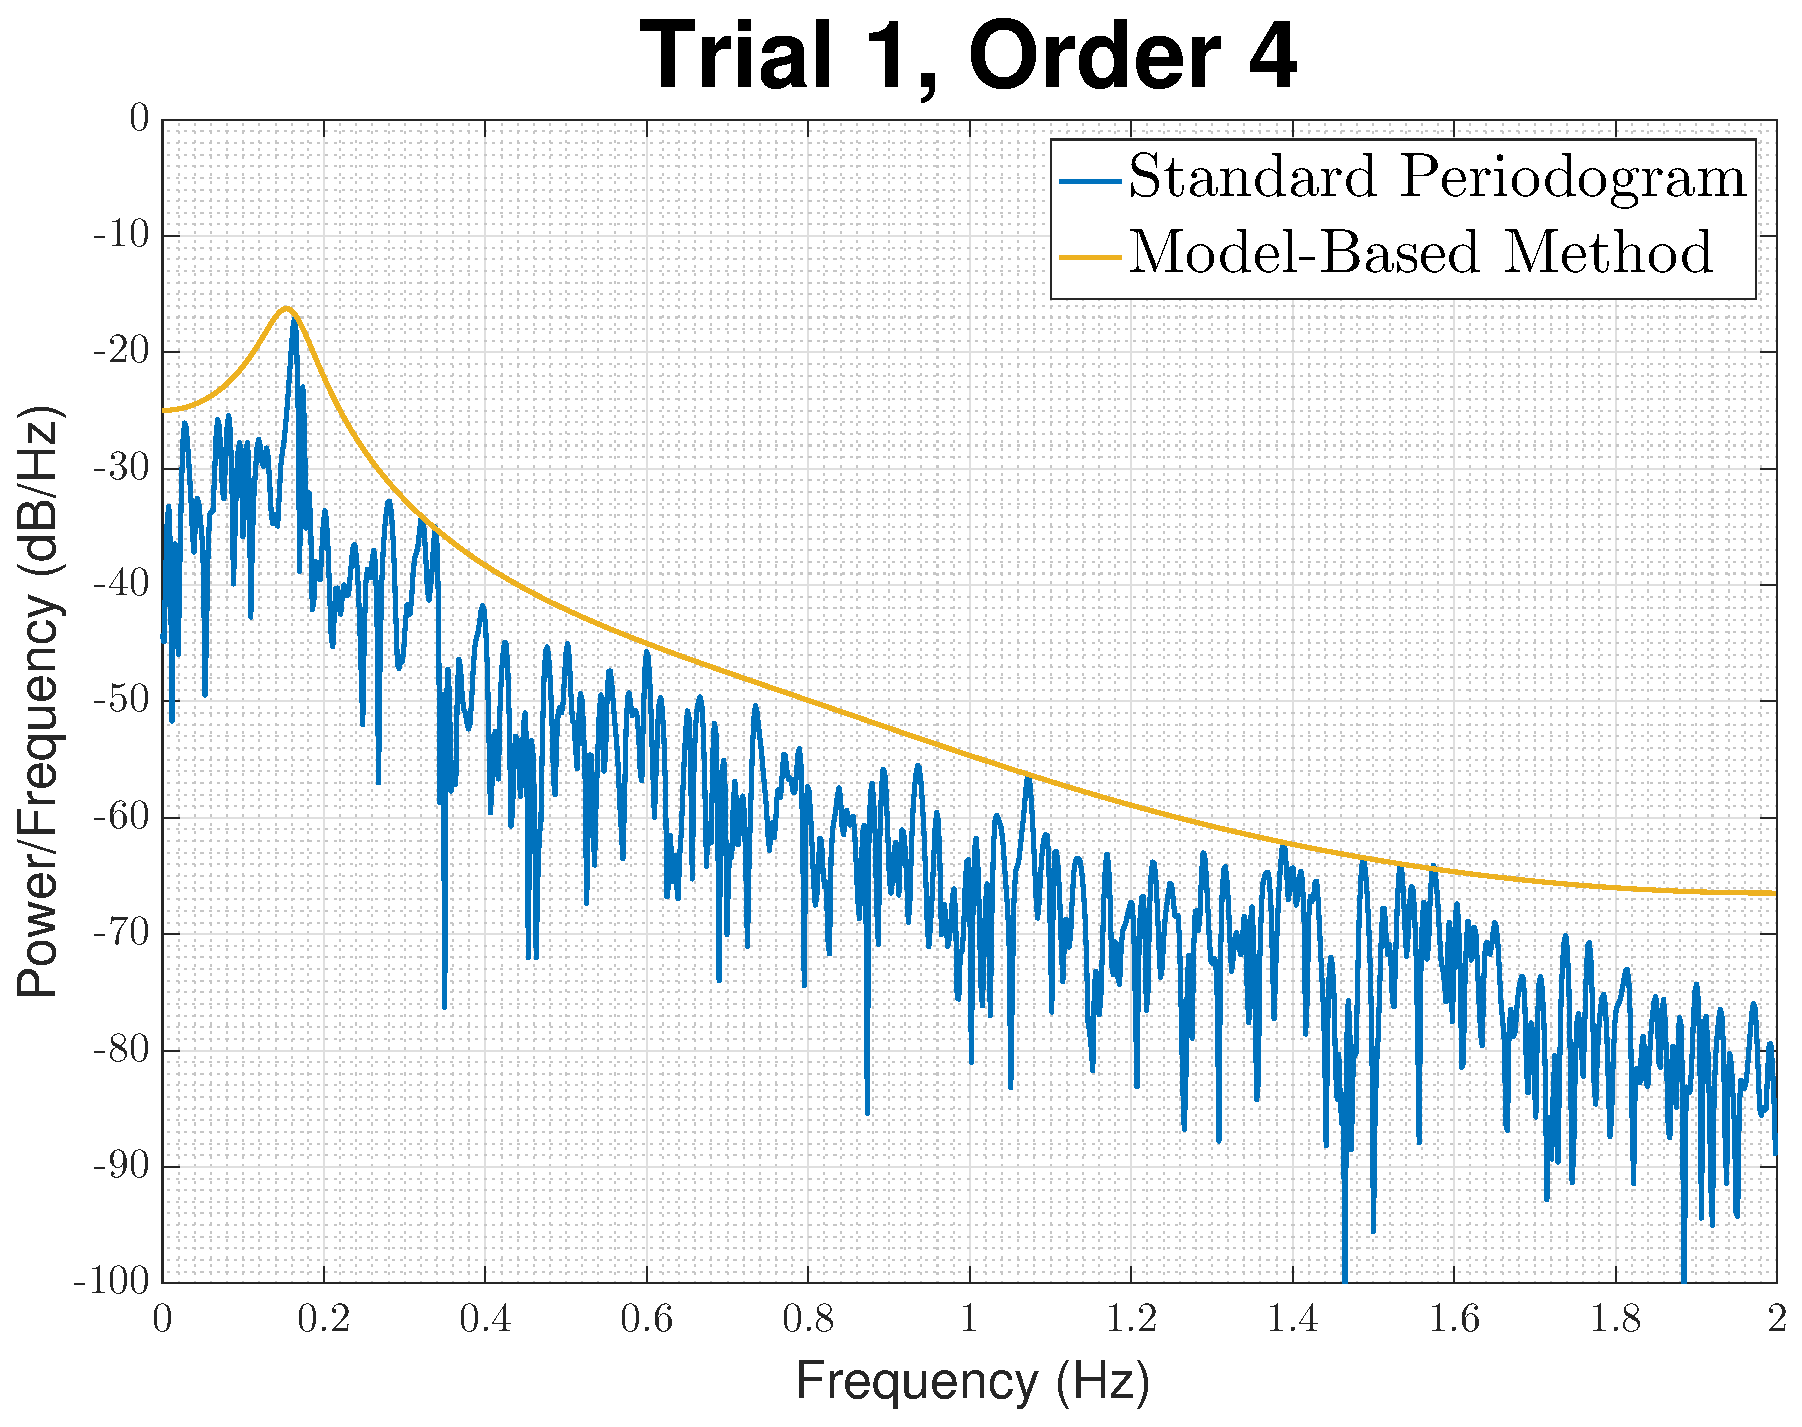
\includegraphics[width=0.32\textwidth]{part2/ar_spectrum_eeg_trial_1_order_4}
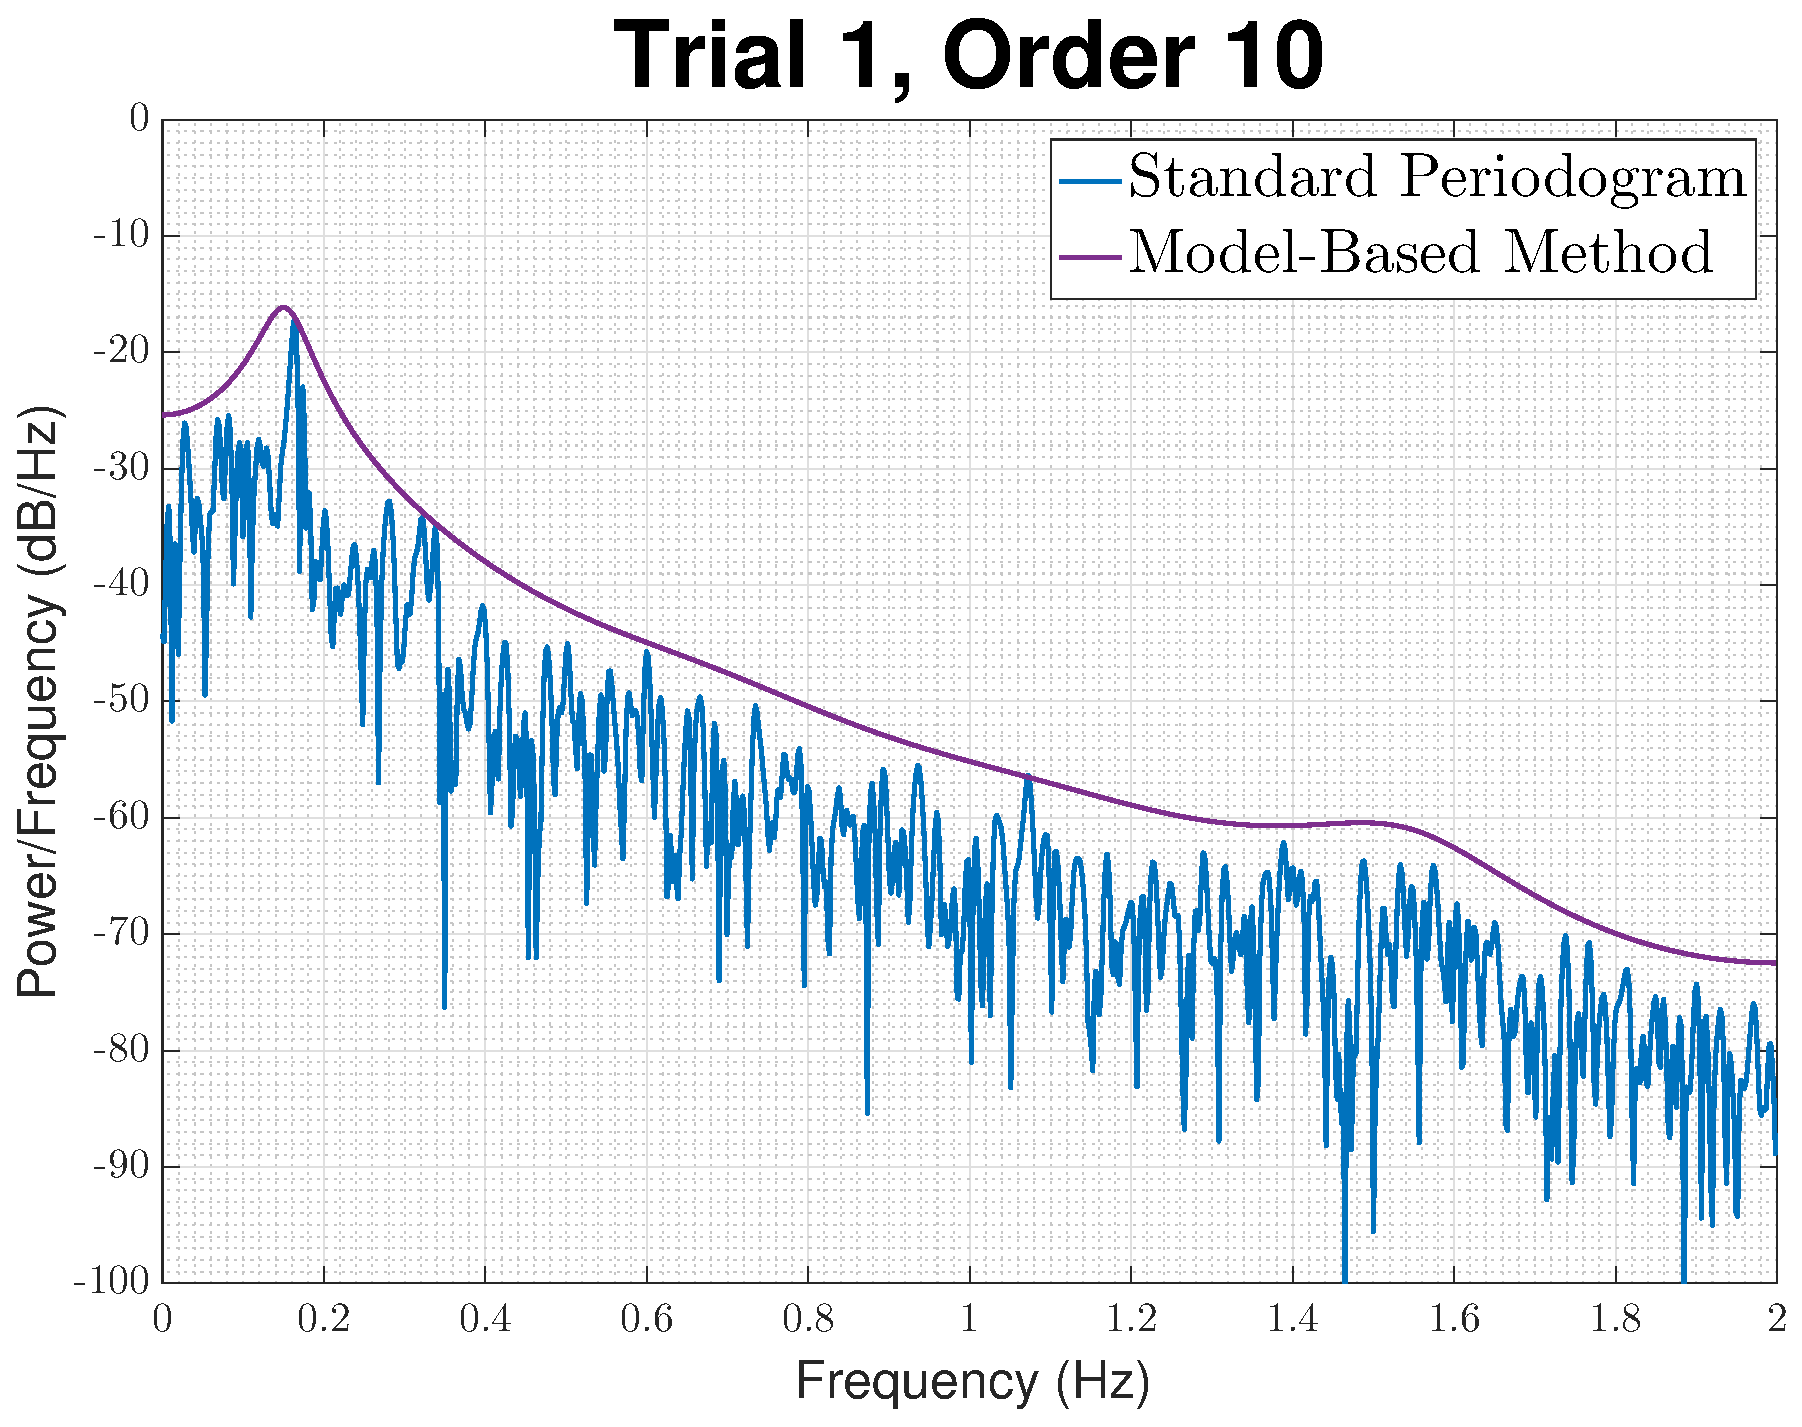
\includegraphics[width=0.32\textwidth]{part2/ar_spectrum_eeg_trial_1_order_10}
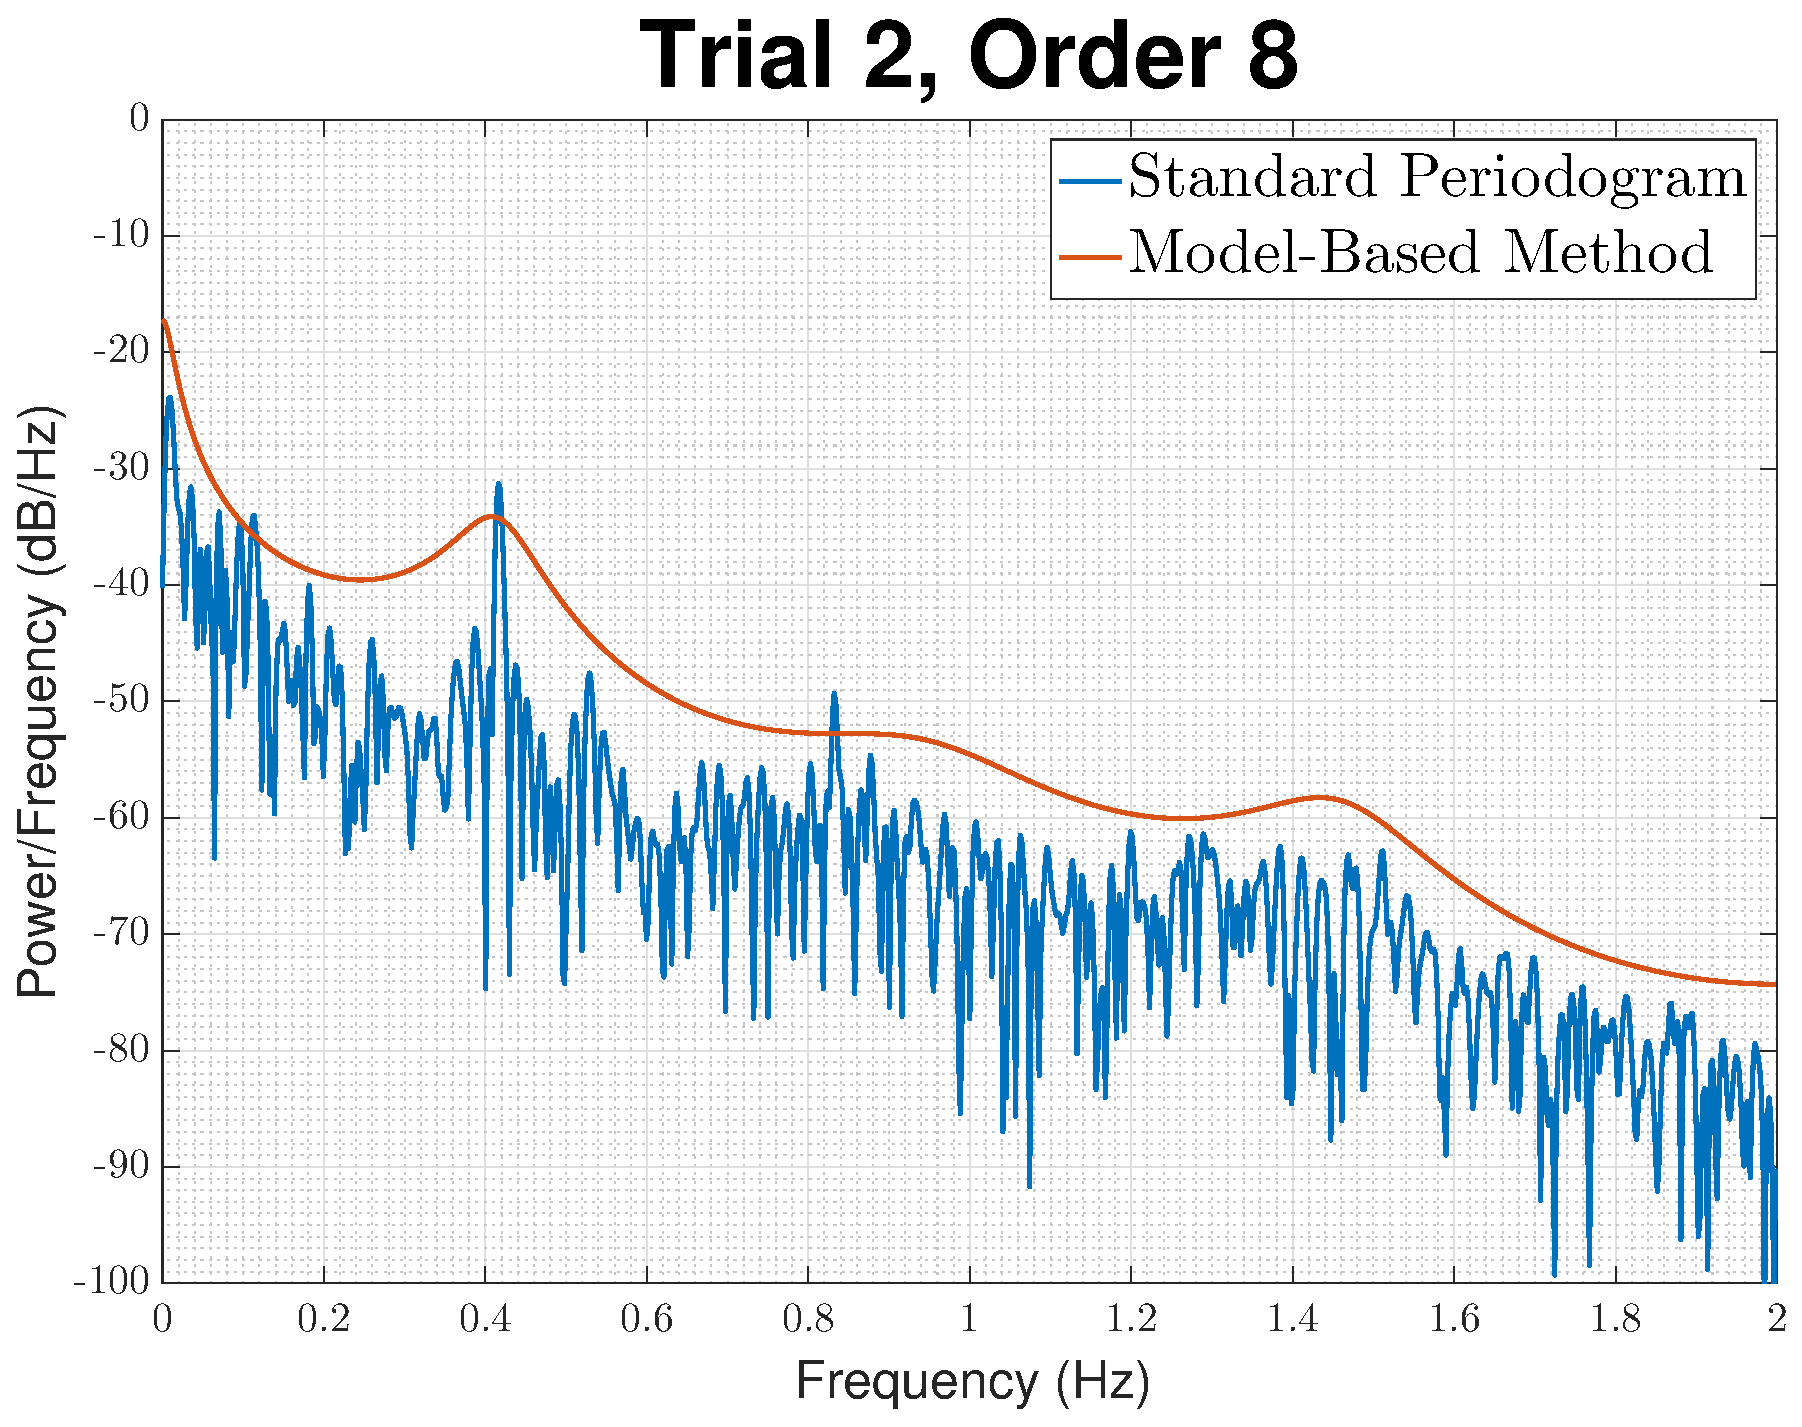
\includegraphics[width=0.32\textwidth]{part2/ar_spectrum_eeg_trial_2_order_8}
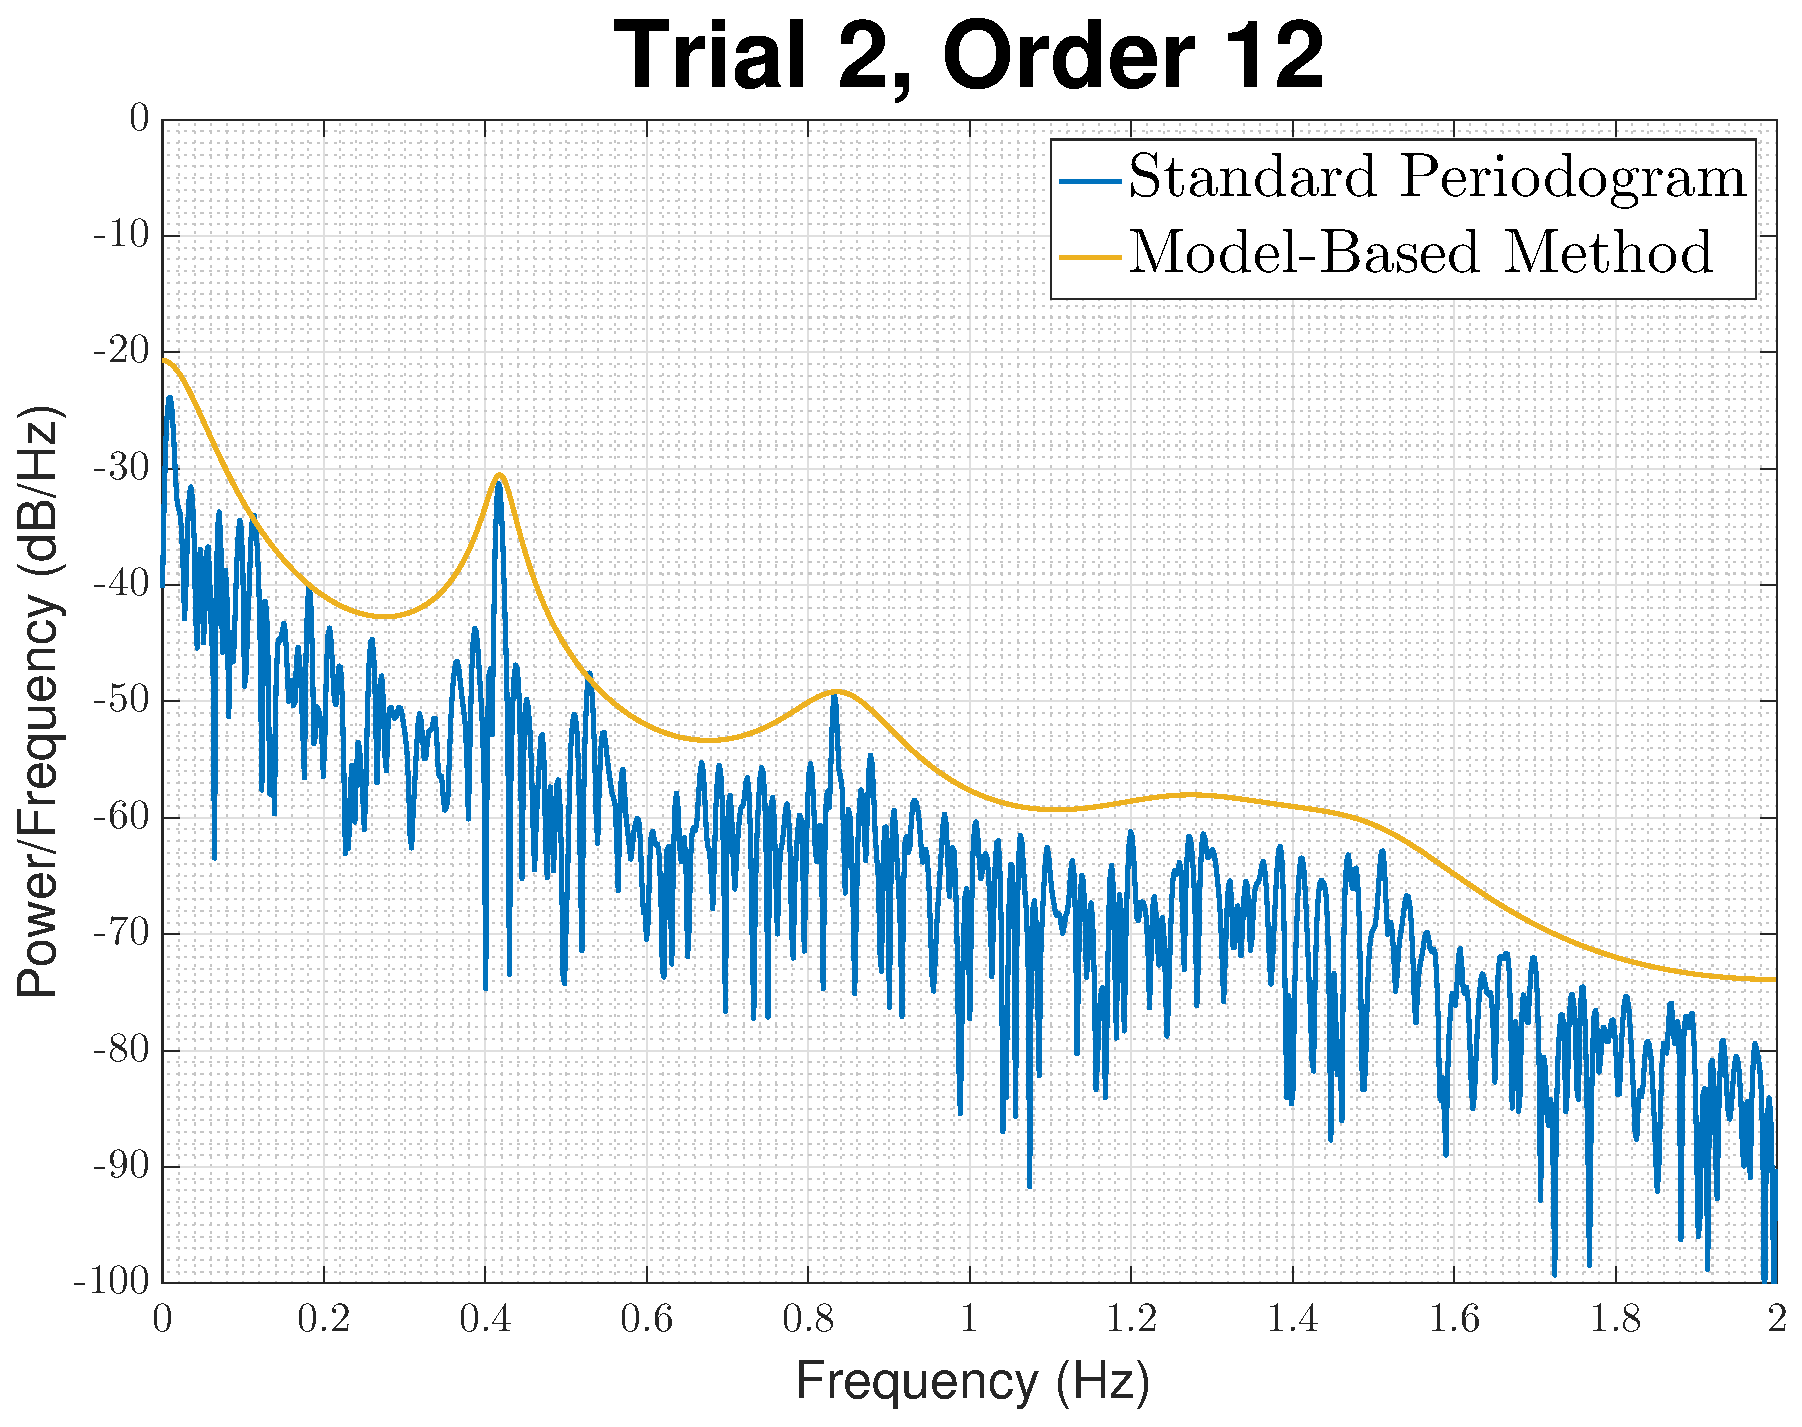
\includegraphics[width=0.32\textwidth]{part2/ar_spectrum_eeg_trial_2_order_12}
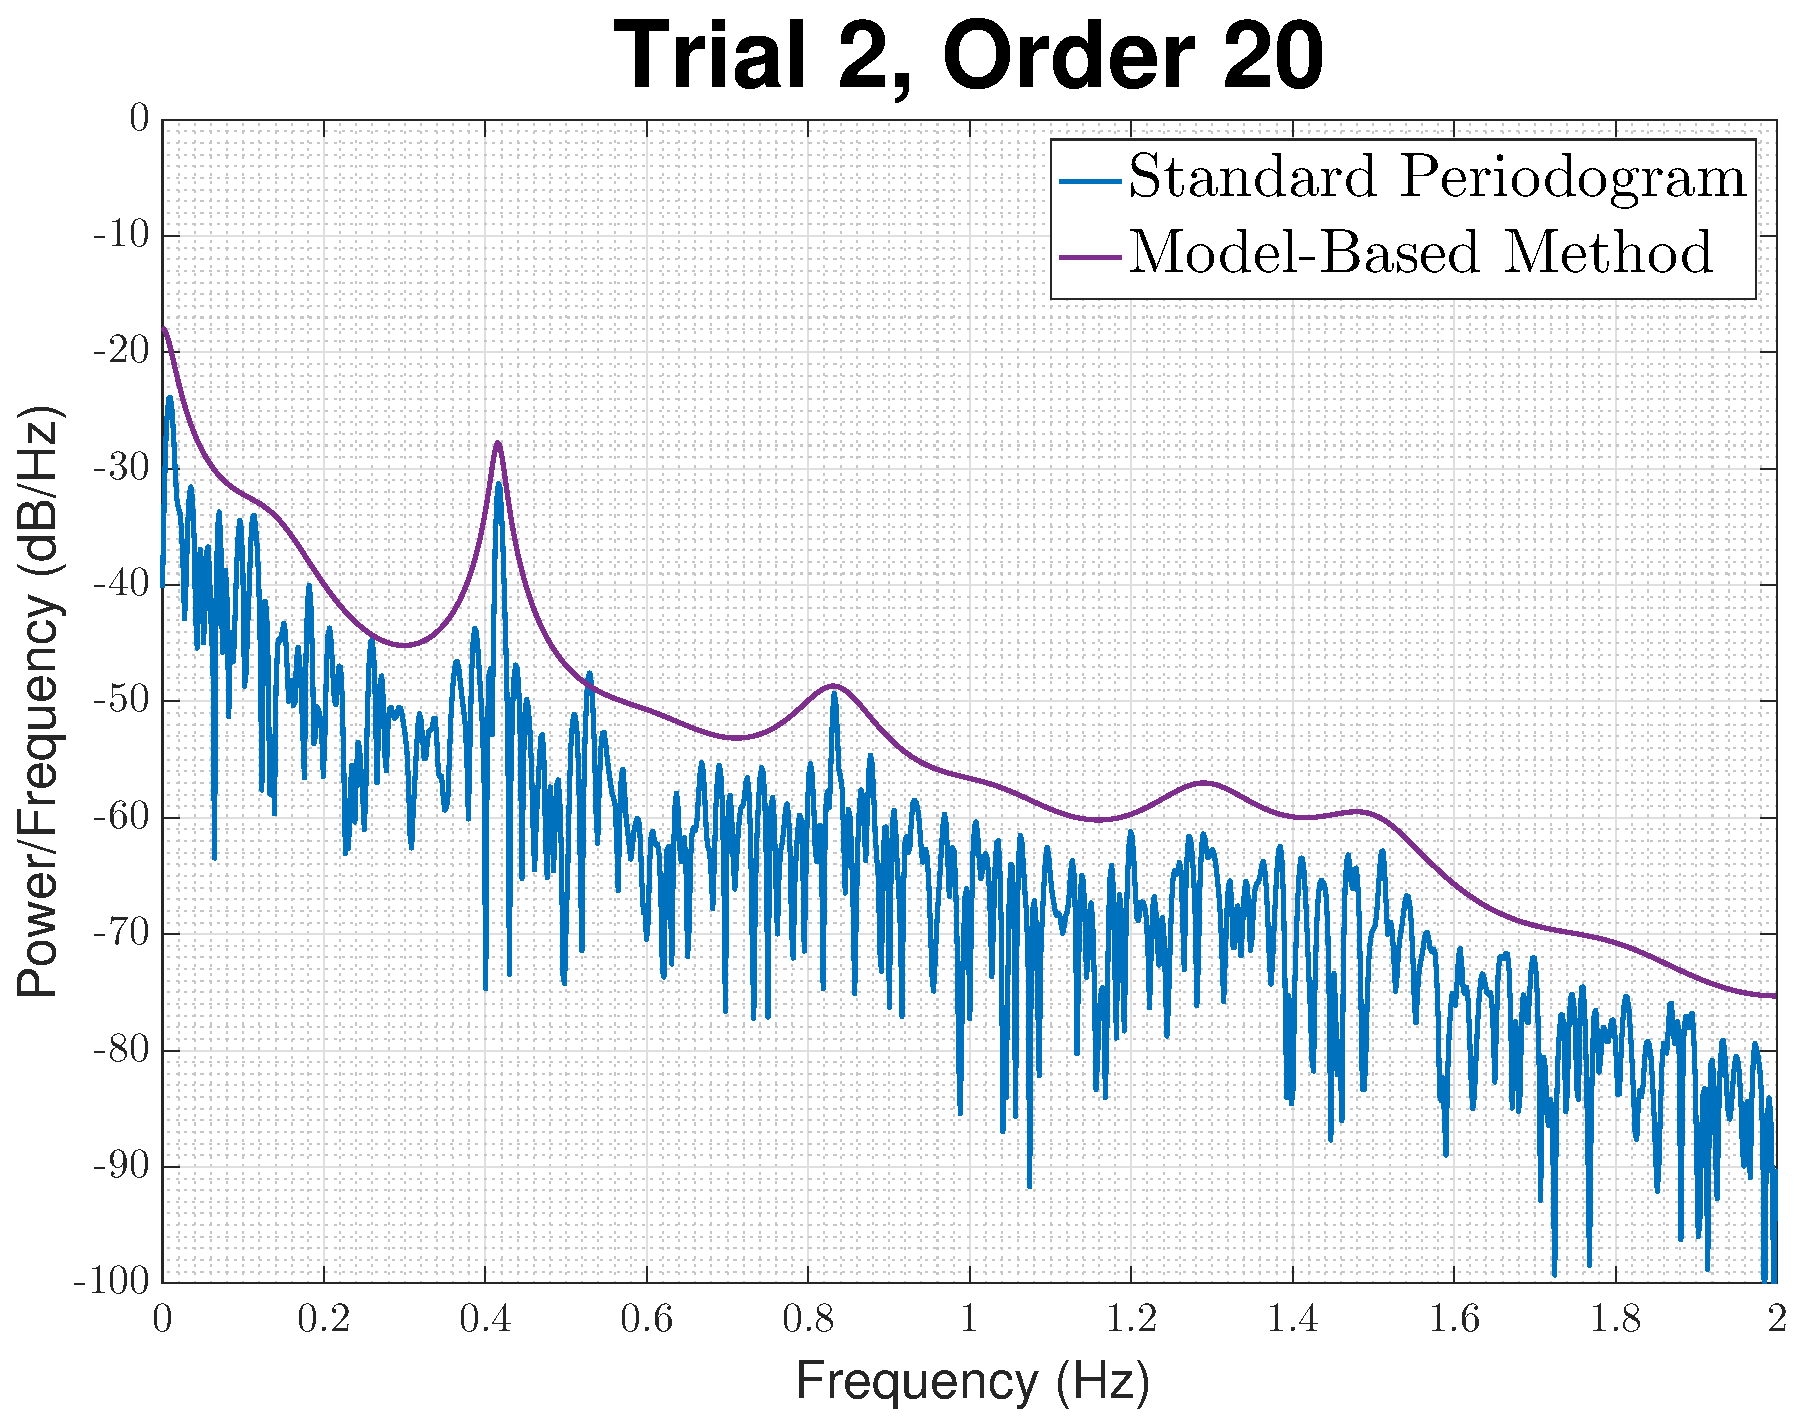
\includegraphics[width=0.32\textwidth]{part2/ar_spectrum_eeg_trial_2_order_20}
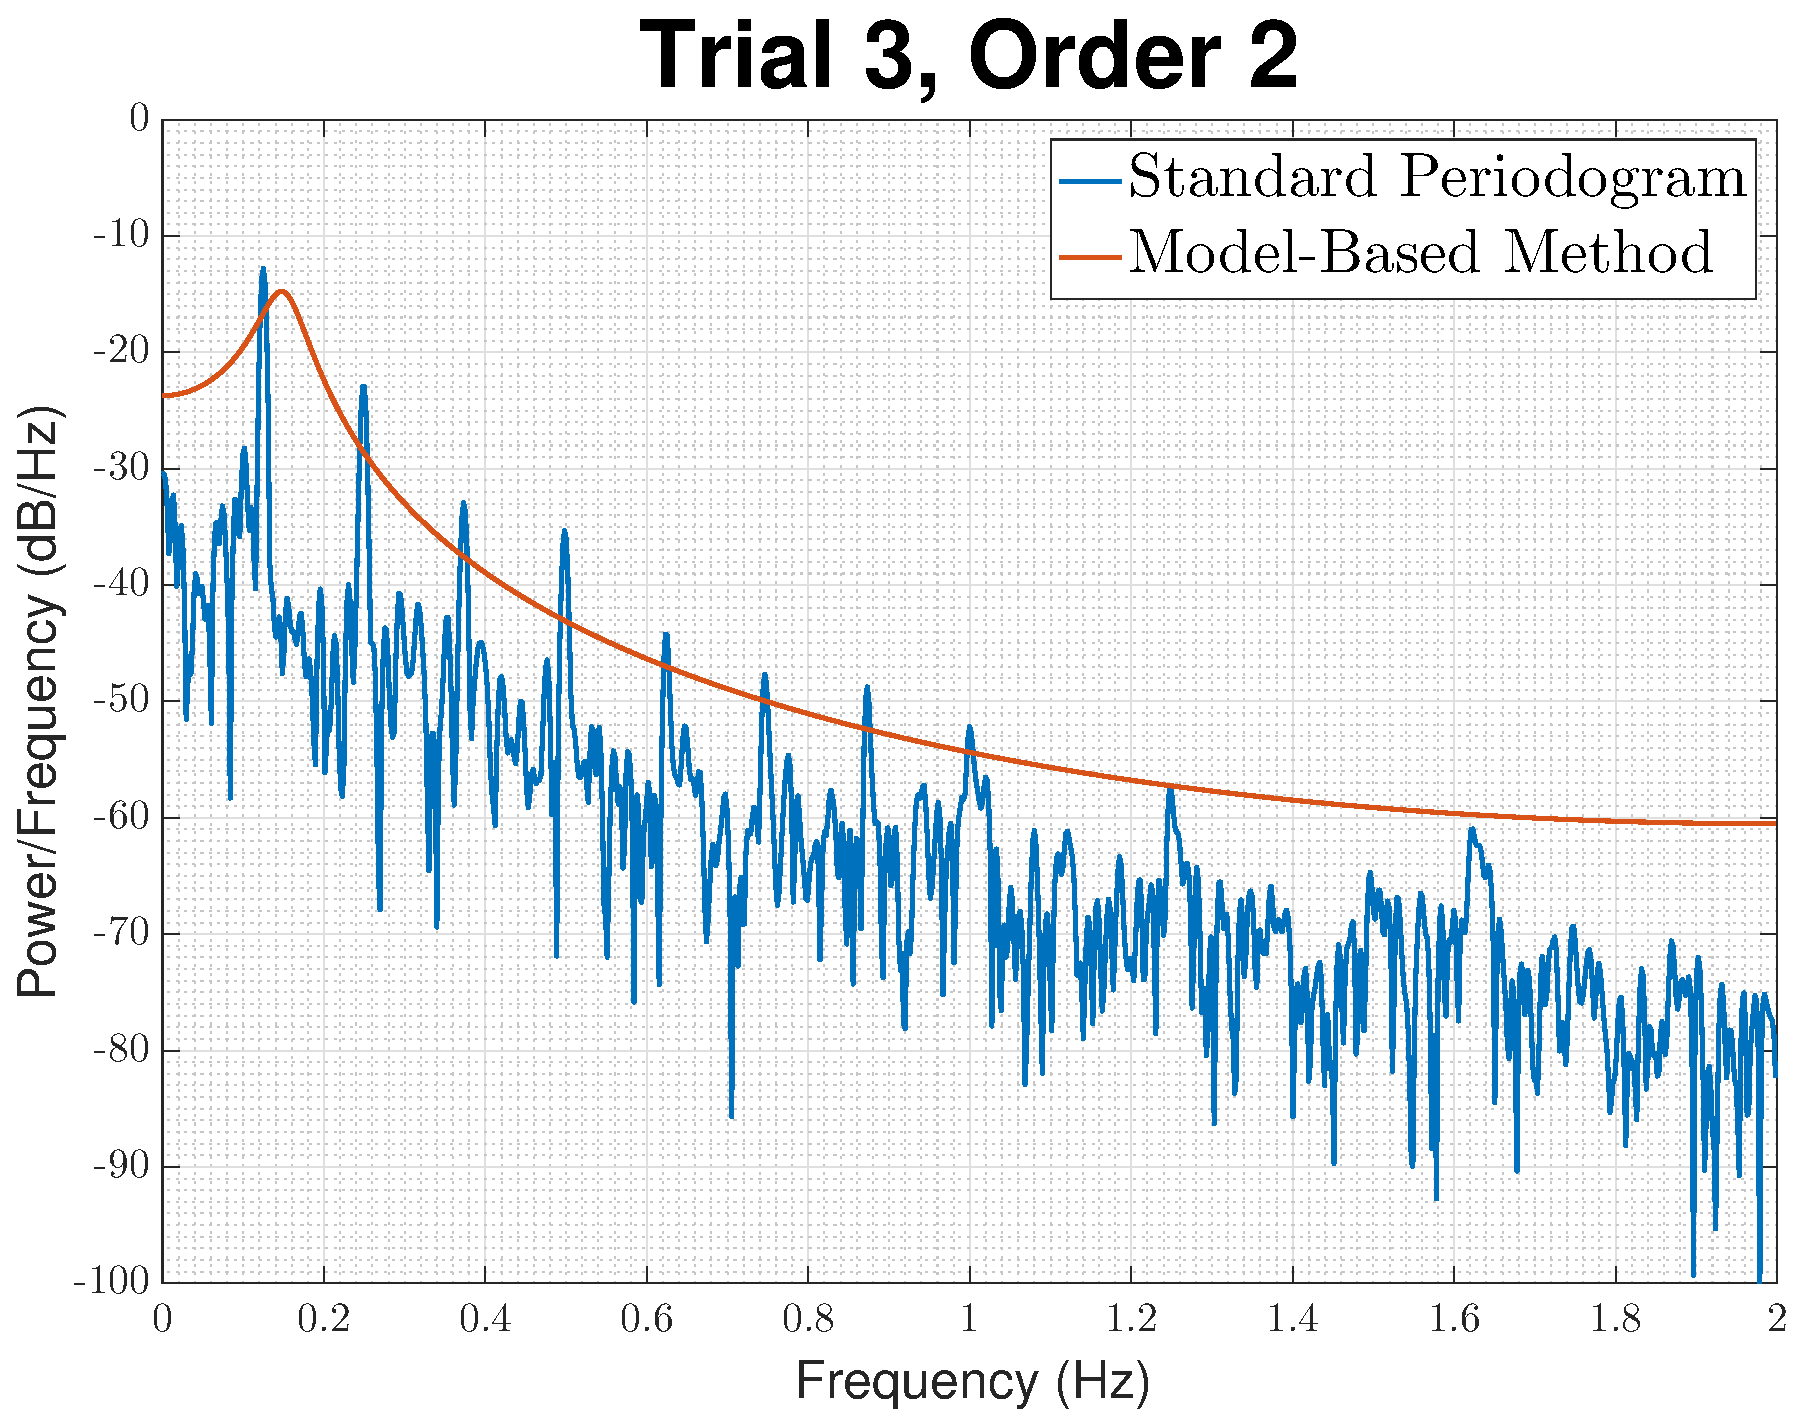
\includegraphics[width=0.32\textwidth]{part2/ar_spectrum_eeg_trial_3_order_2}
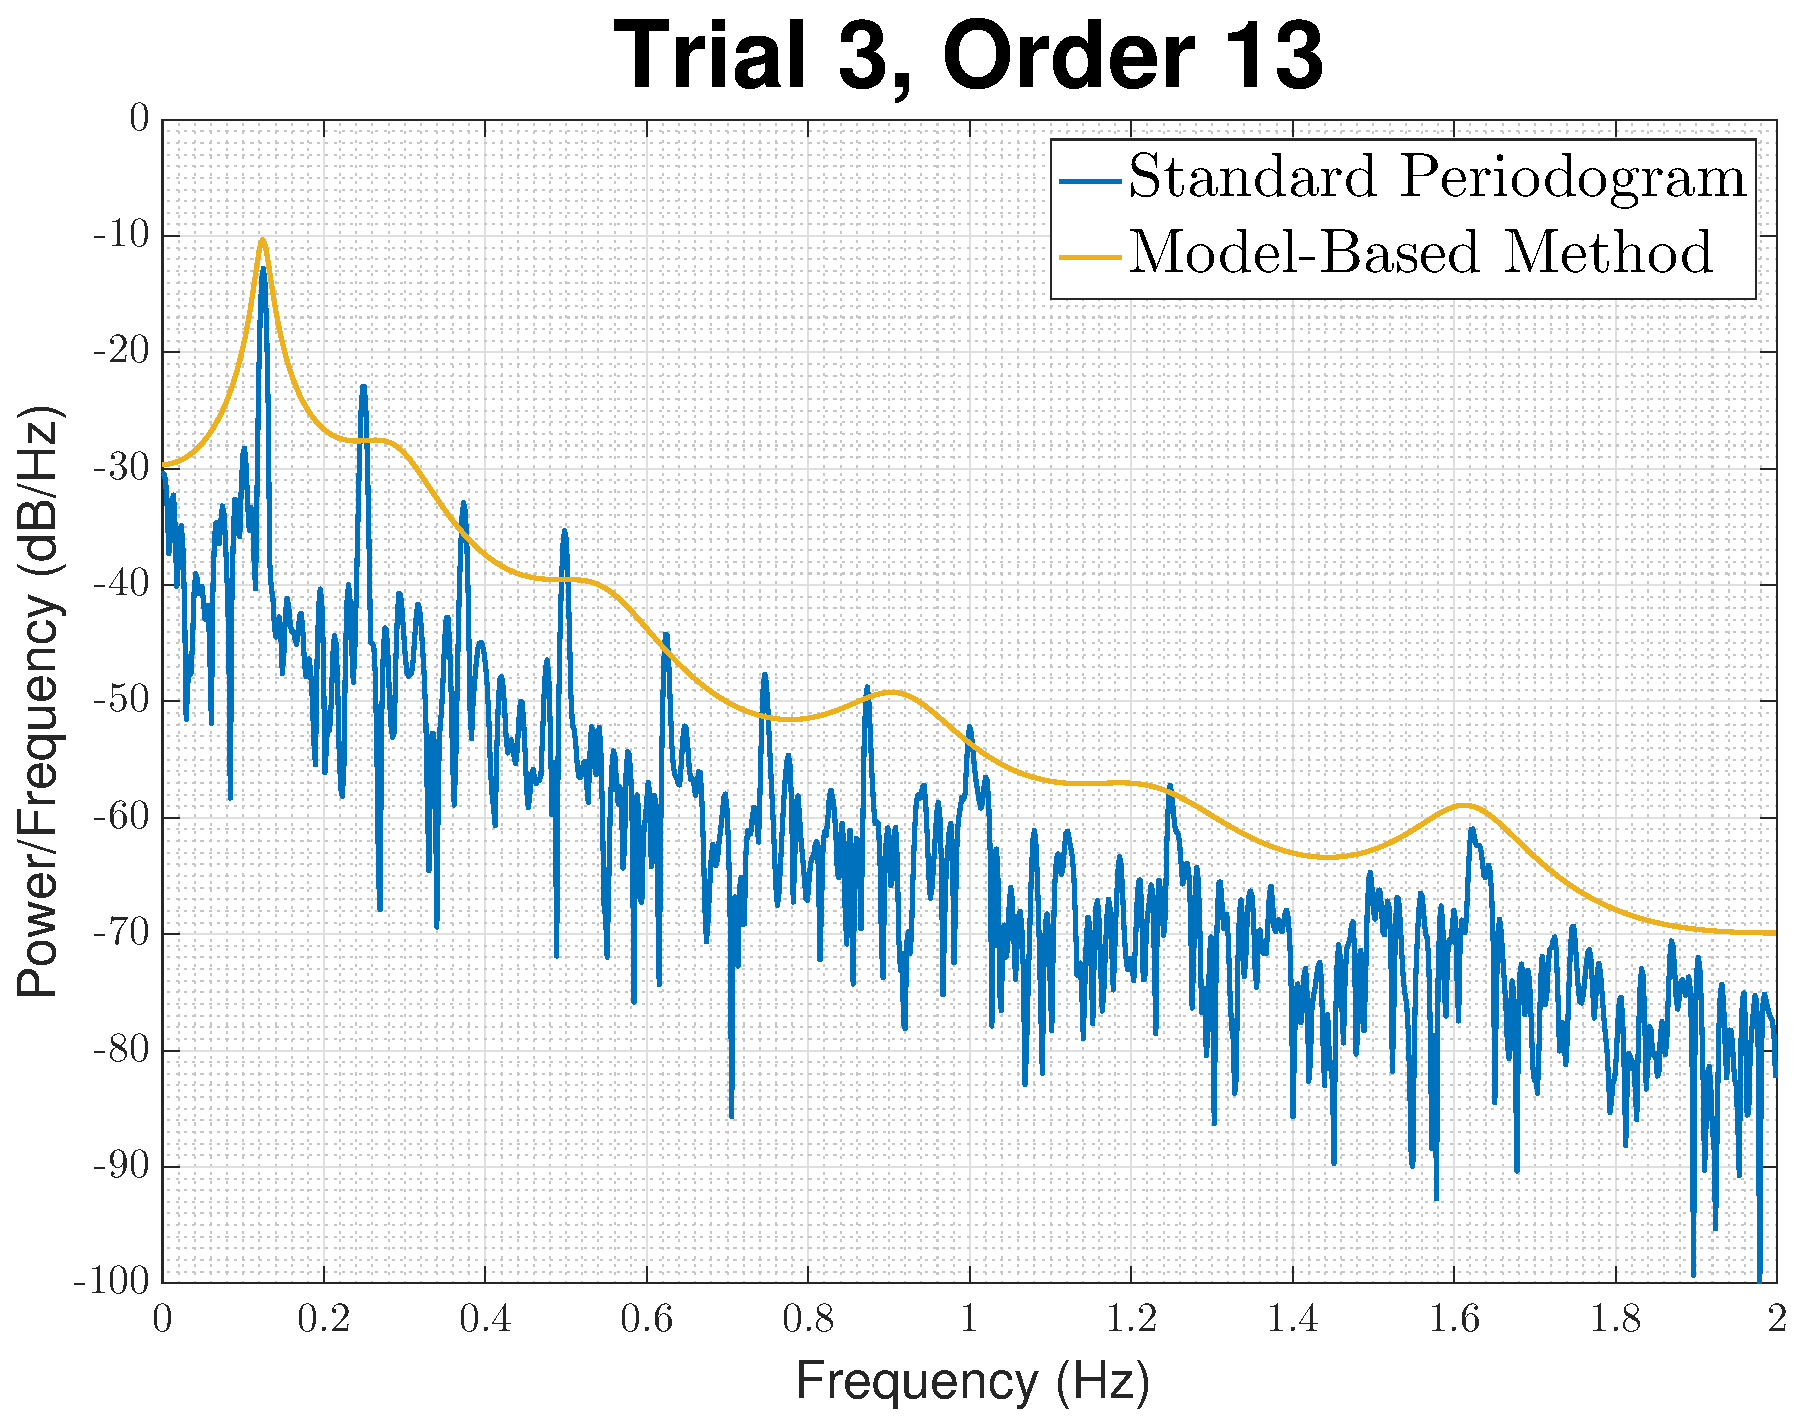
\includegraphics[width=0.32\textwidth]{part2/ar_spectrum_eeg_trial_3_order_13}
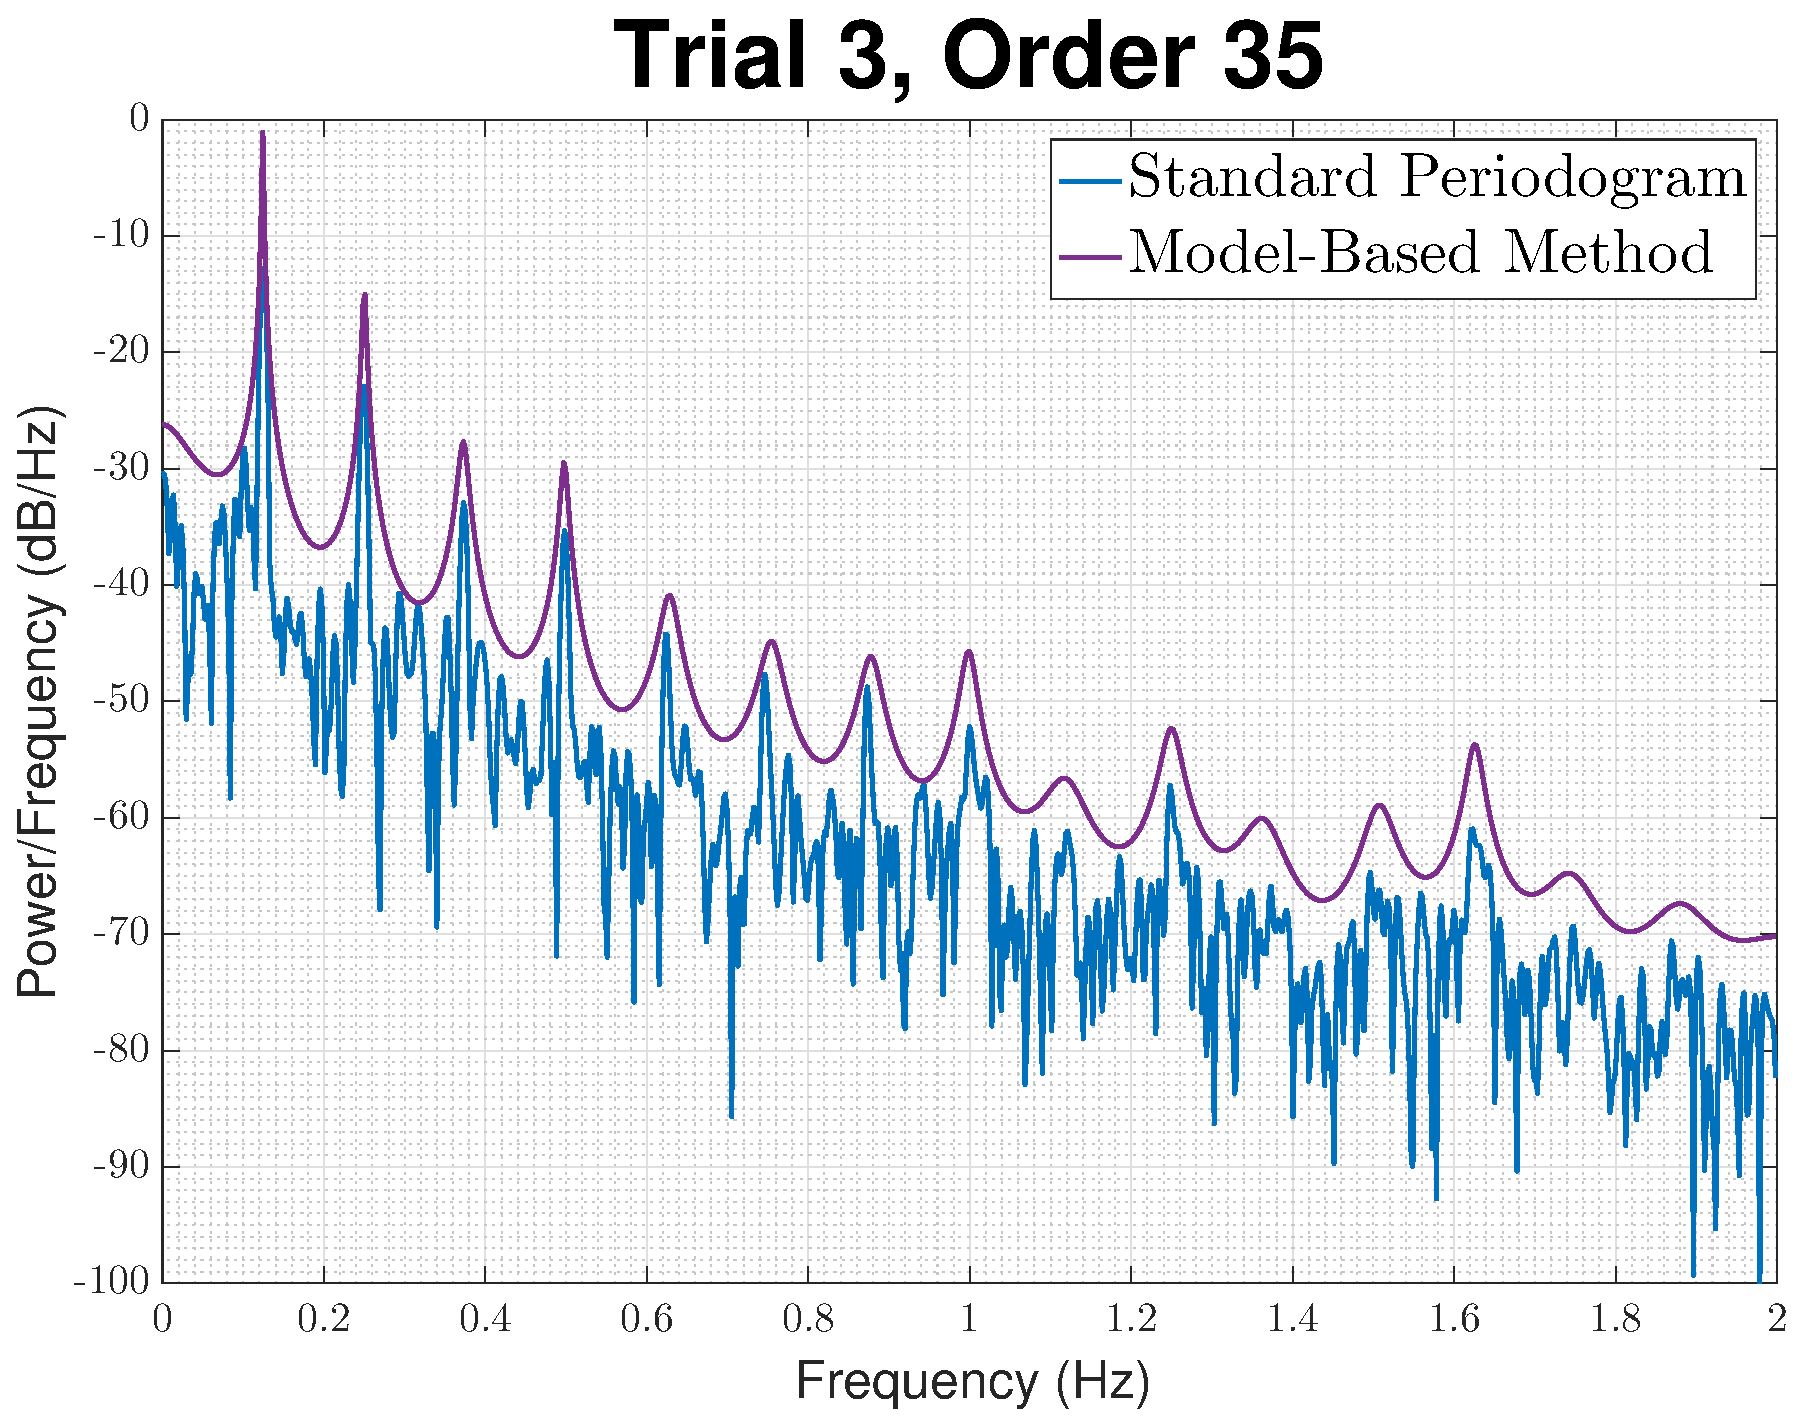
\includegraphics[width=0.32\textwidth]{part2/ar_spectrum_eeg_trial_3_order_35}
\caption{Autoregressive Spectrum Estimate for Trial 1,2,3 for Models for Different Model Orders}
\end{figure}

\noindent{}For Trial 2, it is clear that increasing the model order provides greater degrees of freedom that are able to describe the 2nd and possibly 3rd harmonic well. For Trial 3, similar things are observed. Using an order 35 model, all the peaks can be accurately modeled. Although it is possible to replicate the peaks observed in the standard periodogram, a very high model order is required and this is usually not a good idea as real-world process usually do not have that much memory.\\

\noindent{}Note that, although the AR model based spectrum has its short-comings described above, in general the estimates are very smooth and only tiny offsets/artifacts are observed.

